\documentclass[12pt,a4paper]{report}

\usepackage{enumitem}
\usepackage[utf8x]{inputenc}
\usepackage[francais]{babel}
\usepackage[T1]{fontenc}
\usepackage{amsmath}
\usepackage{amsfonts}
\usepackage{amssymb}
\usepackage[square,sort,comma,numbers]{natbib}
\usepackage[colorlinks=true,linkcolor=blue]{hyperref}
\usepackage{glossaries}
\usepackage[usenames,dvipsnames]{xcolor}
\usepackage{setspace}
\usepackage{graphicx}
\usepackage[rightcaption]{sidecap}
\usepackage{subfigure}
\usepackage{float}
\usepackage[skip=2pt,font=scriptsize]{caption}
\usepackage{listings}
\usepackage{xcolor}
\usepackage[top=2cm, bottom=3cm, left=2cm , right=2cm]{geometry}
\usepackage{multirow}
\usepackage{colortbl}
\usepackage{rotating}

\author{Nicolas JEANNE}
\title{Métabolisme de l'ARN messager dans les opérons : Rôle des BIME chez \textit{Escherichia coli.}}
\date{Juin 2015}

% Mise en page des citations
\bibliographystyle{abbrvnat}
\setcitestyle{authoryear,open={(},close={)},aysep={},citesep={;}}


% formattage des entrées du glossaire
%\renewcommand*{\glstextformat}[1]{\emph{#1}}
% création des acronymes du glossaire
\newacronym{rep}{REP}{Repeated Extragenic Palindrome}
\newacronym{bime}{BIME}{Bacterial Interspesed Mosaic Element}
\newacronym{sra}{\texttt{SRA}}{Sequence Read Archive}
\newacronym{ngs}{NGS}{Next Generation Sequencing}
\newacronym{sam}{\texttt{SAM}}{Sequence Alignment Map format}
\newacronym{bam}{\texttt{BAM}}{Binary Alignment Map format}
\newacronym{gff}{\texttt{GFF}}{General Feature Format}
\newacronym{bed}{\texttt{BED}}{Browser Extensible Data}
\newacronym{de}{DE}{Diff\'erence d'Expression}
\newacronym{rpkm}{RPKM}{Reads Per Kilobase per Million mapped reads}
\newacronym{pdp}{PDP}{Pruned Dynamic Programming}
\newacronym{rig}{RIG}{R\'egion Inter-G\'enique}
\newacronym{et}{ET}{\'Elements Transcriptionnels}

% création des entrées du glossaire
\newglossaryentry{PE}{name={Paired-end sequencing},description={Technique de séquençage haut débit consistant à réaliser les amplifications d'un fragment d'ADN en marquant l'extrémité 5' par un tag \no1 et l'extrémité 3' par un tag \no2. La distance entre les 2 tags est connue et fixe (négative ou jusqu'à 500 pb). Ceci permet lors de l'assemblage, de séquences de 35 pb par exemple, d'associer le read 1 et le read 2 grâce à la distance séparant les 2 et cela même si la séquence intermédiaire est inconnue. Si la distance est négative, il est possible d'obtenir des reads chevauchants de longueur plus importante que les 35 pb}}
\newglossaryentry{SE}{name={Single-end sequencing},description={Technique de séquençage haut débit la plus simple consistant à ne réaliser le séquençage que depuis une extrémité du template.}}
\newglossaryentry{reads}{name={reads},description={Séquence nucléotidique issue d'un séquençage NGS}}
\newglossaryentry{GRanges}{name={Genomic Ranges},description={Format de stockage d'informations pour les éléments génomiques sous R. L'information minimale requise est le chromosome, les positions de départ et de fin, le sens du brin. Ces champs peuvent être suivis de méta-datas où d'autres informations libres peuvent être enregistrées}}
\newglossaryentry{chimerique}{name={alignement chim\'erique},description={Alignement d'un read qui ne peut pas être représenté comme un alignement continu. Un alignement chimérique est représenté comme un ensemble d'alignements, par exemple lorsqu'une partie d'un read est mappé à un locus du génome et la suite à un autre locus}}
\newglossaryentry{couverture}{name={couverture},description={Appelé également profondeur de séquençage, correspond au nombre de reads alignés sur une région génomique. Dans le cas du RNAseq, la couverture fournit une information sur le taux d'expression d'un élément génomique}}
\newglossaryentry{nb}{name={loi Binomiale N\'egative},description={Si une expérience consiste en une série de tirages indépendants  avec une probabilité de succès $p$ et une probabilité d'échec complémentaire, celle-ci se poursuit jusqu'à l'obtention de $n$ succès, la variable aléatoire représentant le nombre d'échecs avant l'obtention des $n$ succès suit une loi négative binomiale. Les paramètres de cette loi sont $n$ le nombre de succès attendus et $p$ la probabilité d'un succès}}
\newglossaryentry{operon}{name={op\'erons},description={unité d'ADN fonctionnelle regroupant des gènes sous le contrôle d'un signal moléculaire régulateur. Les gènes sont transcrits en ARN messager ensemble et concourent à la réalisation d'une même fonction physiologique. Ainsi, soit tous les gènes d'un opéron sont transcrits tous ensemble, soit aucun n'est transcrit puisqu'ils sont tous sous le contrôle du même régulateur}}
\newglossaryentry{tiling-array}{name={tiling-array},description={Cette technique diffère des micro-arrays traditionnels par la nature des sondes, au lieu de disposer de sondes pour des séquences de gènes connues ou prédits, elle sonde des séquences connues pour être disposées dans des régions contiguës et ainsi détecter la présence ou l'absence des transcrits dans ces régions}}
\newglossaryentry{RNA-Seq}{name={RNA-Seq},description={Technique de séquençage haut-débit pour l'étude de l'expression de l'ARN. Un échantillon d'ARN est rétro-transcrit puis amplifié par PCR, le cDNA est séquencé sur un séquenceur haut-débit. Le compte des \gls{reads} produits mappé sur un transcrit représente son abondance}}
\makeglossaries

% Encadrement des figures
\floatstyle{boxed}
\restylefloat{figure}

% Configuration des liens
\hypersetup{
  colorlinks,
  citecolor=Violet,
  linkcolor=Black,
  urlcolor=Blue}

% Configuration des parties de code
\lstset{basicstyle=\small}

\begin{document}

\maketitle

\begin{onehalfspace}
\chapter*{Introduction}
En 1982, la découverte par Higgins de nouveaux éléments génétiques communs dans les régions intercistroniques des opérons de \textit{Escherichia coli} et \textit{Salmonella typhimurium} a constitué le premier pas de la recherche sur les \gls{rep} \citep{Higgins1982}. En 1991, Gilson \textit{et al.} ont mis en évidence l'organisation en clusters de ces REP \citep{Gilson1991}. Ces clusters ont été appelés \gls{bime}. Chez \textit{E. coli} en 1994, Bachelier et son équipe ont réussi à catégoriser les REP constituant les BIME en 2 types Y et Z, constituants 3 motifs Y, Z\textsuperscript{1}, Z\textsuperscript{2}  \citep{Bachellier1994}.
 
Les REP constituent une part non négligeable du génome bactérien, chez \textit{E. coli} K12 ou \textit{S. typhimurium} elles représentent environ 1\% de celui-ci \citep{Gilson1991}. Nous les retrouvons chez de nombreux règnes bactériens, notamment chez les pathogènes humains tels que \textit{E. coli, Salmonella enterica, Neisseria meningitidis, Mycobacterium tuberculosis et Pseudomonas aeruginosa} mais également chez des pathogènes des plantes comme \textit{Agrobacterium tumefaciens} ou chez des bactéries ubiquitaires, \textit{Deinococcus radiodurans} ou \textit{Pseudomonas putida} par exemple. Les travaux précédents de l'équipe ont permis l'annotation des REP au sein des génomes d'\textit{E. coli} et \textit{Shigella} et de mettre en évidence le lien existant entre la prolifération des REP et le gène $tnpA_{REP}$ \citep{Weyder2013,Bosc2014}, ainsi que la reconstruction des états ancêtres des REP \citep{Bosc2014}.  \textcolor{red}{Le rôle exact des REP n'est pas clairement défini, des hypothèses sont avancées sur leur implication dans la régulation de l'expression des gènes, que ce soit en tant que terminateur de transcription ou comme site de reconnaissance des enzymes impliquées dans les mécanismes de la transcription.}

\section*{Caractéristiques des REP et organisations en BIME}

\begin{figure}[ht]
\centerline{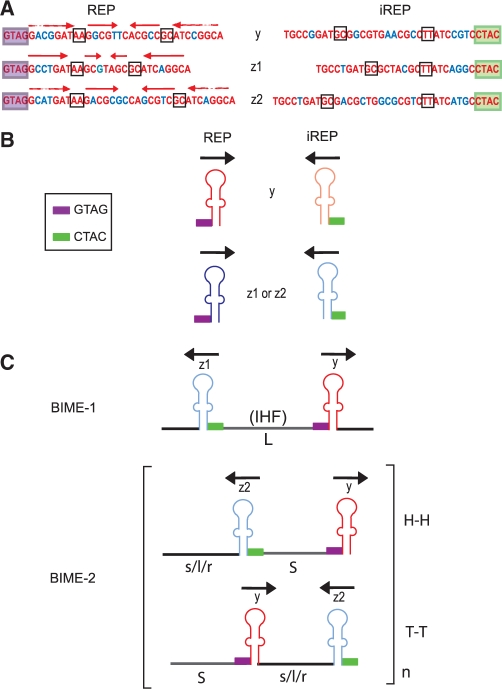
\includegraphics[scale=0.5]{figures/rep_bime.jpg}}
\caption{\textbf{REP et BIME chez \textit{Escherichia coli}. (A)} Séquences consensus Y, Z\textsuperscript{1} et Z\textsuperscript{2} des REP. Le tétra-nucléotide conservé GTAC est encadré en violet, le complémentaire conservé CTAC est encadré en vert, les flèches rouges situent les zones d'appariement de la tige et les positions encadrées en noir sont les zones de mésappariement. Les positions conservées parmi les classes de REP sont en rouge, les positions variables en bleu. \textbf{(B)} Structure secondaire des REP. Les rectangles violets et verts représentent respectivement les tétra-nucléotides conservés GTAC pour les REP et CTAC pour les iREP. Les flèches noires indiquent l'orientation des REP. \textbf{(C)} Structures des BIME-1 et BIME-2. Les BIME-1 sont composées de REP et de iREP Y et Z\textsuperscript{1} séparées par un linker de séquence longue (L), les BIME-2 sont composées de Y et Z\textsuperscript{2}, de linker courts (S) et de séquences séparatrices s, l ou r. H-H et T-T dénotent respectivement une organisation tête à tête et queue à queue des REP. \citep{Ton-Hoang2012}.}
\label{fig:rep_bime} 
\end{figure}

Chez \textit{E. coli}, la taille des REP est d'environ 40 nucléotides, la classification Y, Z\textsuperscript{1}, Z\textsuperscript{2} est basée sur leur séquence primaire. Par convention, une REP en orientation inversée est nommée iREP (inversed REP) \citep{Ton-Hoang2012}. Un tétra-nucléotide caractéristique de séquence GTAC est présent à l'extrémité 5' des REP, sa séquence complémentaire est CTAC en 3' pour les iREP. Les séquences consensus des différentes classes de REP partagent des nucléotides conservés (\autoref{fig:rep_bime}A). La structure secondaire des REP est caractérisée par sa forme en tige-boucle, le caractère palindromique permet la formation de la tige malgré un mésappariement situé dans la partie centrale de celle-ci (\autoref{fig:rep_bime}B) permettant la reconnaissance par $tnpA_{REP}$. Une classification a été adoptée comportant 3 classes \citep{Bachellier1997}, les BIME-1 composées de REP Z\textsuperscript{1} et Y apparaissant en paires uniques. Les BIME-2 constituées de Z\textsuperscript{2} et de Y, apparaissant en copies multiples de cette paire. La troisième catégorie est constituée des BIME dites atypiques qui sont des chimères de BIME-1 et BIME-2, comportant différentes combinaisons de Y, Z\textsuperscript{1}, Z\textsuperscript{2}. Tout comme les BIME-2, nous les retrouvons sous forme de copies multiples (\autoref{fig:rep_bime}C). Les REP peuvent former des structures secondaires avec elles-même, mais également entre elles lorsqu'elles sont organisées sous forme de BIME \textcolor{red}{à quel endroit cette figure? (\autoref{fig:malEF_rep})}.

\begin{figure}[ht]
\centerline{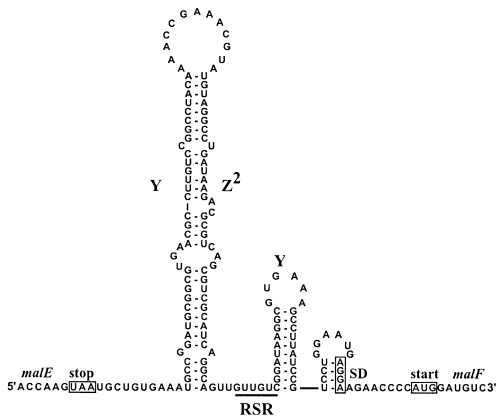
\includegraphics[scale=0.5]{figures/malEF_rep.png}}
\caption{\textbf{Structure ARN des REP au sein de l’opéron \textit{malEFG}.} Y, Z\textsuperscript{2} et Y indiquent la séquence des REP dans l'espace inter-génique de malE-malF. Bien que Y et Z\textsuperscript{2} puissent former des structures tige-boucles par elles mêmes, elles s'apparient ensemble pour former une région étendue en grande partie à double brin (70\% des nucléotides sont appariés). La séquence affichée provient du génome d'\textit{E. coli K12}. La région REP-stabilized RNA (RSR) indique l'extrémité 3′ du messager malE mature, qui s'étend de 3 à 9 nucléotides depuis la base de la tige-boucle formée par Y et Z\textsuperscript{2}. Les codons STOP de  malE et START de malF sont encadrés. SD représente la séquence Shine–Dalgarno nécessaire à l'initiation de la traduction de malF. \citep{Khemici2004}.}
\label{fig:malEF_rep} 
\end{figure}

\section*{Propriétés associées aux REP}
La littérature décrit de nombreuses fonctions hypothétiques associées aux REP au niveau structurel du génome, au niveau de l'ADN et au niveau de l'ARN. Sur un plan structurel, les REP ont été décrites comme jouant un rôle dans les événements de \textbf{recombinaisons homologues} \citep{Kofoid2003} et les BIME ont été décrites comme des sites privilégiés pour \textbf{l'insertion de séquences d'ADN mobiles} comme certaines familles d'IS (Insertion Sequence) \citep{Bachellier1997,Clement1999,Choi2003,Tobes2005}. Au niveau de l'ADN, les REP sont capables de \textbf{lier plusieurs facteurs protéiques} tels que l'ADN Gyrase \citep{Espeli1997} et l'ADN polymérase \citep{Gilson1990}. Plus spécifiquement, la BIME-1 peut \textbf{lier l'\textit{IHF} sur son linker} \citep{Boccard1993} qui peut être notamment responsable de l'\textbf{initiation de la transcription et d’événements de recombinaisons sites spécifiques} \citep{Goosen1995}. Au plan de l'ARN, lorsqu'elles sont transcrites, les REP joueraient un rôle dans la \textbf{stabilisation de l'ARNm} grâce à leur structure en tige-boucle \citep{Newbury1987,Espeli2001,Khemici2004,Aguena2009}, la \textbf{terminaison de la transcription} \citep{Gilson1986} et \textbf{le contrôle de la traduction} \citep{Stern1988}. 

\section*{ARN messagers chez \textit{E. coli}}

\subsection*{Unités de transcription}
L'étude des unités de transcription (UT), également appelées \gls{operon}, est difficile de par leur complexité. Des approches globales ont révélé que la presque totalité du génome était transcrit et parfois dans les deux orientations. Il apparaît également que les gènes peuvent être transcrits à partir de plusieurs promoteurs et que la terminaison de la transcription pouvait également se produire à différentes positions. Ce dernier point suggère que les terminateurs de transcription sont sujets à des fuites plus ou moins importantes (cas extrêmes des atténuateurs de transcription). D'autre part, il existe peu d'évidences expérimentales directes de l'organisation en opérons, même dans le génome d'\textit{E. coli}. Par contre, avec le développement d'approches globales d'étude de la transcription des gènes, il devient possible de prédire la localisation des sites d'initiation et de terminaison de la transcription. Ces informations couplées à d'autres propriétés génomiques comme la distance inter-génique permet de prédire l'organisation en opérons des gènes.

\subsection*{Stabilité des ARNm}
La dégradation des ARNm chez \textit{E.coli} est réalisée par l'intervention du dégradosome. Il s'agit d'un complexe multi-enzymatique composé de quatre protéines majeures, la RNase E, la PNPase, la RhlB et l'Enolase (\autoref{fig:degradosome}).

\begin{figure}[ht]
\centerline{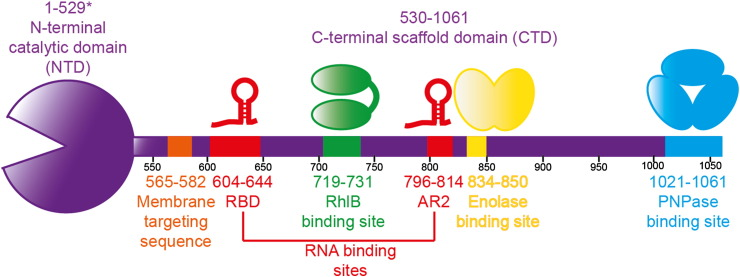
\includegraphics[scale=4]{figures/degradosome.jpg}}
\caption{\textbf{Structure du dégradosome.} Représentation canonique du dégradosome, la partie violette symbolise la RNase E avec le domaine catalytique à gauche, la partie verte le site de liaison de la RhlB, la jaune celui de l'Enolase et la bleue celui de la PNPase \citep{Bandyra2013}.}
\label{fig:degradosome} 
\end{figure}

Un élément clé dans la dégradation du transcrit chez \textit{E. coli} est que celle-ci débute toujours par un clivage réalisé par une endoribonucléase (RNase E). Une fois clivés, les transcrits sont complètement dégradés par des exoribonucléases (RNase R, RNase II ou PNPase) dégradant l'ARNm par l'extrémité 3' et par des oligoribonucléases grâce à la coopération de nombreuses enzymes telles que la poly(A) polymérase (PAP) et les RNA hélicases qui facilitent l'accès aux fragments d'ARN. La RNase E possède une affinité pour les substrats possédant une extrémité mono-phosphate en 5'. Les transcrits primaires bactériens possèdent une extrémité 5' tri-phosphate qui les protège de la dégradation jusqu'à ce qu'ils soient déphosphorylés par l'activité des pyrophosphohydrolases. La RNAse E reconnaît alors l'extrémité 5' mono-phosphate des transcrits par contact de son domaine catalytique \citep{Callaghan2005,Bandyra2013}.

\begin{SCfigure}[][h!]
\fbox{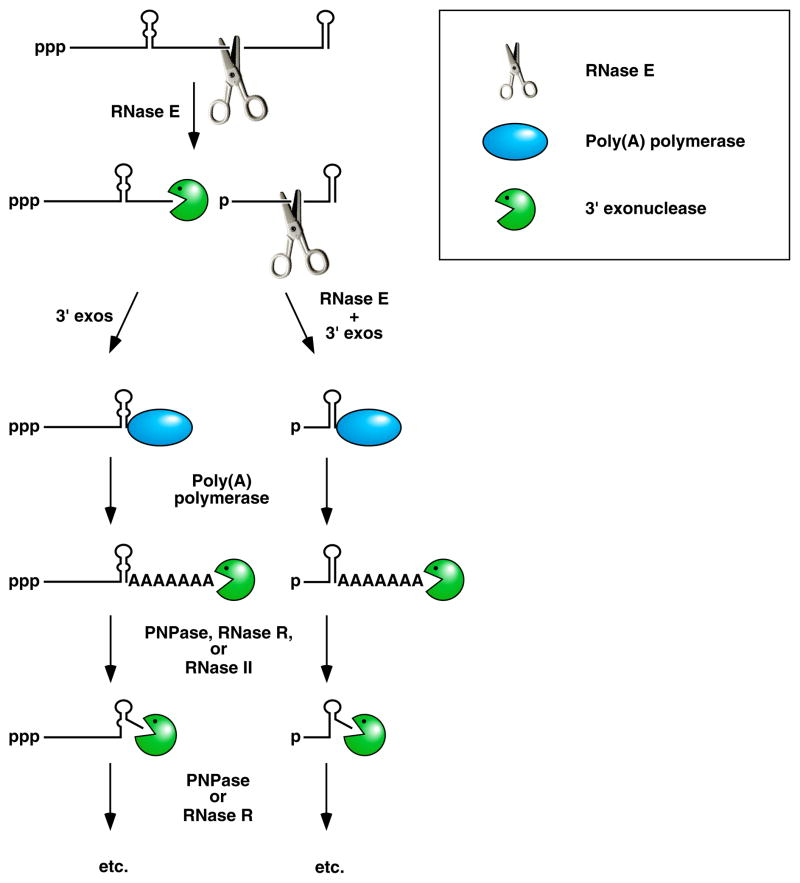
\includegraphics[scale=0.65]{figures/mrna_degradation.jpg}
\caption{\textbf{Facilitation de la dégradation des ARNm chez \textit{E. coli} par l'intervention de polyadénylation.} Le clivage endonucléolytique par la RNase E génère de multiples fragments, dont certains possèdent à leur extrémité 3' une structure en tige-boucle. Ces fragments subissent une digestion de leur extrémité 3' par la PNPase, la RNase II et/ou la PNPase jusqu'à ce que cette structure soit rencontrée interrompant la dégradation. La PAP intervient pour déstabiliser la tige boucle par l'ajout d'une séquence poly-A en 3' autorisant la reprise de la dégradation par la PNPase et/ou la RNase R \citep{Belasco2010}.}
\label{fig:mrna_degradation} }
\end{SCfigure}

La présence de structure secondaires telles que peuvent en former les REP peut entraver le processus de dégradation initié par les exoribonucléases, la PAP intervient alors en ajoutant sur l'extrémité 3' du transcrit une séquence poly-A qui va déstabiliser la structure secondaire et permettre ainsi aux exoribonucléases de poursuivre la dégradation (\autoref{fig:mrna_degradation}).

\subsection*{Terminaison de la transcription}
Le mécanisme de terminaison de la transcription chez les procaryotes est gouverné par deux classes signaux de fin de transcription. Les terminateurs Rho-dépendant dont l'activité s'appuie sur la liaison de la protéine Rho à un site \emph{rut} (Rho utilization) présent sur le transcrit associé à une interaction avec la RNA Polymérase et les terminateurs Rho-indépendants caractérisés par une structure G-C riche formant une tige-boucle suivie d'une série de résidus U. Ces terminateurs peuvent être bi-directionnels (\autoref{fig:terminator}) \citep{Henkin2000,Lesnik2001}.  

\begin{SCfigure}[][h!]
\fbox{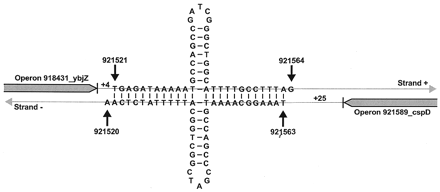
\includegraphics[scale=0.65]{figures/terminator.png}
\caption{\textbf{Terminateur Rho-indépendant bi-directionnel.} La région riche en G-C constitue la structure en tige, la boucle étant formée par les bases non appariées. A la suite de cette structure, nous observons la répétition de T (U) caractéristique. \citep{Lesnik2001}.}
\label{fig:terminator} }
\end{SCfigure}

\section*{Objectifs}
Dans l'état actuel de la recherche beaucoup de pistes pointent vers le fait que les REP joueraient un rôle soit dans la terminaison de la transcription, soit dans le processus de dégradation des \textcolor{red}{transcrits au niveau ARN CITER REFERENCE ou protéique CITER REFERENCE}. \textcolor{red}{L'objectif de ce stage est donc à partir des données d'expression chez \textit{E. coli} de découvrir si les REP et leur organisation en BIME sont impliquées dans ces processus de terminaison de transcription et/ou de stabilisation de la partie 5' du transcrit.} Différentes technologies sont disponibles pour étudier l'expression des gènes, les principales sont le micro-array, le \gls{tiling-array} et le \gls{RNA-Seq}. Notre choix s'est porté sur le RNA-Seq car il présente plusieurs avantages sur les autres technologies. A la différence des arrays, cette technologie ne nécessite pas la synthèse de sondes spécifiques des espèces ou des transcrits, elle peut donc détecter de nombreux événements non attendus. Elle offre des seuils de détection beaucoup plus bas car elle ne souffre pas du bruit spécifique aux arrays ce qui améliore sa spécificité et sa sensibilité. La profondeur de séquençage permet de détecter des transcrits rares et de faible abondance. Notons que ces approches fournissent une estimation de l'expression des gènes qui est la résultante de la transcription et de la dégradation des ARNm.

Concernant le RNA-Seq, nous pouvons distinguer deux approches. L'une qui consiste à analyser les données d'expression de mutants par rapport à un individu sauvage ou une population dans des conditions standards et une population dans des conditions perturbées. Et l'autre, alternative, où pour une même condition, nous nous intéressons à la \textbf{différence de niveau d'expression d'un gène par rapport à un autre}. Dans le cas d'un opéron, nous nous attendons à ce que les gènes qui le constituent possèdent un profil d'expression similaire. Cette approche est privilégiée pour notre étude puisque nous cherchons à étudier le rôle des REP dans le métabolisme de l'ARN.
A notre connaissance, il n'existe pas d'approche globale sur l'implication des REP dans l'expression des gènes co-transcrits. Nous avons développé des méthodes pour tenter de découvrir le rôle des REP en nous basant sur des données d'expressions issues d'expériences de RNA-Seq. \textcolor{red}{La première d'entre elles est une méthode statistique permettant de tester l'expression des gènes des opérons. Les deux suivantes recherches des points de cassures dans la couverture des reads dénotant des changements de niveaux d'expression. La première approche cherche les corrélations entre un profil d'expression provenant des données de séquençage et un profil théorique signifiant un point de cassure. L'autre est une méthode de segmentation détectant également les points de cassure mais n'utilisant plus de corrélation. Les résultats de ces trois méthodes sont croisées et le sous-ensemble résultant sera ensuite étudié du point de vue de la stabilité des structures secondaires en comparant les séquences actuelles avec celles reconstruites de leurs séquences ancêtres.}


\chapter*{Matériel \& Méthodes}

Les données d'expression de RNA-Seq sont récupérées au format \texttt{fastq}, qui est un pré-traitement des données brutes des séquenceurs, fournissant pour chacun des \gls{reads} un identifiant, sa séquence et le score de qualité de chacune des bases la composant. Pour travailler sur les données d'expressions, nous devons convertir ces informations de séquences en table de comptage représentant l'expression des gènes du génome, ces étapes sont détaillées sur la \autoref{fig:data_preparation}.

\begin{SCfigure}[][h!]
\fbox{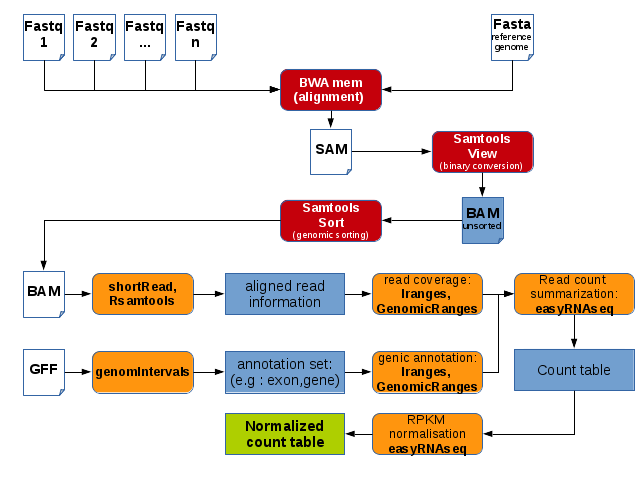
\includegraphics[scale=0.75]{figures/data_preparation.png}
\caption{\textbf{Déroulé de l'analyse pour obtenir la table de comptage normalisée.} Pour le modèle choisi sur notre analyse, les fichiers d'entrée sont en blanc, les traitements avec des logiciels externes à \texttt{R} sont en rouge, les traitements par les packages \texttt{R} sont colorés en orange, les données intermédiaires en bleu et la table de comptage normalisée produite est en vert.}
\label{fig:data_preparation}}
\end{SCfigure}

\section*{Jeux de données}
Plusieurs jeux de données ont été utilisés, tous issus d'expériences RNA-Seq publiées, accessibles sur le base de données \href{http://www.ncbi.nlm.nih.gov/geo/}{GEO} (Gene Expression Omnibus) du NCBI au format \gls{sra}. Grâce au \href{http://www.ncbi.nlm.nih.gov/books/NBK158900/#SRA_download.how_do_i_use_the_sra_toolki}{SRA toolkit}, elles sont décompressées au format \texttt{fastq} et un contrôle de qualité est effectué afin d'inspecter les reads grâce au logiciel \texttt{fastqc} (Annexe \ref{annexeCode}).

Le \href{http://www.ncbi.nlm.nih.gov/geo/query/acc.cgi?acc=GSE61327}{premier jeu de données} que nous avons exploité est issu des expériences d'évolution adaptatives en laboratoire visant à découvrir l'émergence de mutations clés permettant la croissance rapide d'\textit{E. coli K-12 MG1655} sur un milieu pauvre en glucose \citep{Lacroix2014}. Ces données ont été choisies car elles proviennent d'expériences de RNA-Seq comportant un nombre important de réplicats (9) pour la condition de croissance en milieu pauvre en glucose (GSE61327\_ALE). Elles ont été obtenues par séquençage sur Illumina MiSeq à partir d'ARN totaux extraits des cultures d'\textit{E. coli} et rétro-transcrit en cDNA. La librairie a été conçue en \gls{PE}. 8 réplicats ont été validés disposant d'une qualité de séquence par base supérieure à 30 pour des reads de 62 pb, seul le fichier \texttt{SRR1573441.fastq} a été rejeté car la longueur des reads allait de 35 à 502 pb avec des scores de qualités très variables.

Le \href{http://bioinfolab.uncc.edu/TruHmm_package/raw_data/}{second jeu de données} provient d'une expérience visant à développer un algorithme pour la détection des opérons chez \textit{E. coli K12} \citep{Li2013}. Nous nous sommes intéressés à celles provenant des cultures ayant subi un choc thermique pendant 15 minutes (HS-15min) ainsi qu'à celles provenant de culture privées de phosphore pendant 4 heures (M-P4h). Ces 2 conditions ont été retenues car elles possèdent 3 réplicats contre 2 pour toutes les autres. Les librairies ont été conçues en \gls{SE} et brin spécifique en utilisant le kit Illumina’s TruSeq Small RNA Sample Prep, puis séquencées à la fois sur Illumina HiSeq 2000 (générant des reads de 100 bases) et Illumina GA II (générant des reads de 76 bases). Aucun réplicat n'a été rejeté suite aux contrôles qualité.

\section*{Fichiers d'annotations}
Dans ce travail, nous avons utilisé l'annotation du génome d'E. coli K12 MG1655, souche pour laquelle le plus grand nombre de données RNA-Seq sont disponibles et servant de référence sur certaines bases de données d'annotation telles que \href{http://regulondb.ccg.unam.mx/}{RegulonDB}.
Le fichier \gls{gff} d'annotation du génome d'\textit{E. coli K12} a été généré par un script Perl à partir du fichier \href{http://www.ncbi.nlm.nih.gov/nuccore/NC_000913.2}{GenBank}. Les fichiers répertoriant les opérons et les promoteurs proviennent de RegulonDB. Pour les opérons, le fichier se compose de 2640 entrées dont 1792 sont constitués d'un seul gène, ces derniers ne  seront pas utilisés dans notre analyse puisqu'elle requiert au moins deux gènes. Parmi les 848 autres, 235 ont été annotés comme ayant de fortes évidences d'existence (expérimentalement vérifiés), les 613 autres présentent des évidences d'existence plus faibles (inférence automatique, bibliographie,\ldots). Le fichier des promoteurs contient 8580 entrées dont 6461 ont été annotées comme présentant des preuves fortes d'existence. Le fichier répertoriant les terminateurs de transcription provient de \href{http://csbl.bmb.uga.edu/DOOR/}{Door\up{2}DB} et contient 1835 entrées, nous n'avons pas d'information sur la manière dont ils ont été annotés. Quant aux REP et BIME, les fichiers d'annotations proviennent de l'équipe. Les REP ont été annotées à l'aide d'une combinaison de méthodes basées sur des profils avec ou non prise en compte de la conservation de la structure secondaire. Elles sont regroupées en BIME si elles sont distantes de moins de 100 pb \citep{Weyder2013}. L'annotation a été réalisée sur 71 génomes complets d'\textit{Escherichia} et de \textit{Shigella}. Pour le génome d'\textit{E. coli K-12}, 605 REP ont été annotées par l'équipe, elles se regroupent en 287 BIME dont 93 sont constituées de REP solitaires.

\section*{Alignement des reads}
Les reads ont été alignés puis mappés sur le génome d'\textit{E. coli} \href{http://www.ncbi.nlm.nih.gov/nuccore/NC_000913.2}{NC\_000913.2}, qui est le génome utilisé pour annoter les REP par l'équipe, grâce au logiciel \href{http://bio-bwa.sourceforge.net/}{BWA}.  Ce logiciel propose 3 algorithmes distincts, \texttt{BWA-backtrack}, \texttt{BWA-SW} et \texttt{BWA-MEM}. Pour chacun de ces alignements, il est nécessaire de disposer de la séquence du génome de référence indexée (Annexe \ref{annexeCode}). 
L'algorithme que nous avons sélectionné est le \texttt{MEM} (Maximal Exact Matches) pour sa rapidité et sa précision. Il reprend les mêmes principes que \texttt{BWA-SW} (utilisation de la programmation dynamique pour trouver les points d'ancrage (seeds) en autorisant les mésappariements (mismatchs) et les brèches (gaps). Il n'étend les alignements des seeds que lorsque ceux-ci ont peu d'occurrences sur le génome de référence, cela permet de diminuer le temps d'alignement en éliminant les extensions des séquences très répétées mais en utilisant l'ancrage avec des \texttt{MEM}, puis il réalise l'extension en prenant en compte les pénalités dues aux gaps et aux mismatchs. Les valeurs par défaut du logiciel ont été utilisées (Annexe \ref{annexeCode}).
Le fichier d'alignement généré est au format \gls{sam}, afin de poursuivre l'analyse il doit être converti au format \gls{bam}, puis des critères de qualité sont appliqués. Seules les séquences possédant une qualité de mapping supérieur à 30, valeur d'usage commun, et n'étant pas étiquetées (taggées) comme \gls{chimerique} sont conservées. Cette opération a aussi le mérite de compresser l'information et ainsi de gagner en espace de stockage. Les séquences sont ensuite triées par position génomique. Finalement, le fichier \texttt{BAM} trié est indexé pour être visualisable sur un Genome Browser. Les outils utilisés sont compris dans la suite des \href{http://samtools.sourceforge.net/samtools.shtml}{samtools}. Pour les besoins ultérieurs de l'analyse, les réplicats d'une même condition sont fusionnés en un seul fichier (Annexe \ref{annexeCode}).

\subsection*{Intégration des données}
Les fichiers d'annotation ont été transformés au format \gls{bed} grâce à des scripts Python.
Ces changements de format permettent de travailler aisément avec la suite de logiciels \href{http://bedtools.readthedocs.org/en/latest/}{BEDtools} permettant de croiser les informations provenant de plusieurs sources de données et ainsi de rechercher des intersections, des positions proches ou déterminer une \gls{couverture} de reads. Ces outils ont généré les fichiers \texttt{BED} qui serviront de référence pour la suite de l'analyse statistique.

\subsection*{Visualisation du mapping}
L'alignement des reads et le mapping sur le génome de référence de \textit{E. coli} sont visualisés grâce au genome browser \href{https://www.broadinstitute.org/igv/}{IGV} \citep{Robinson2011,Thorvaldsdottir2013} (\autoref{fig:igv}).

\begin{SCfigure}[][h!]
\fbox{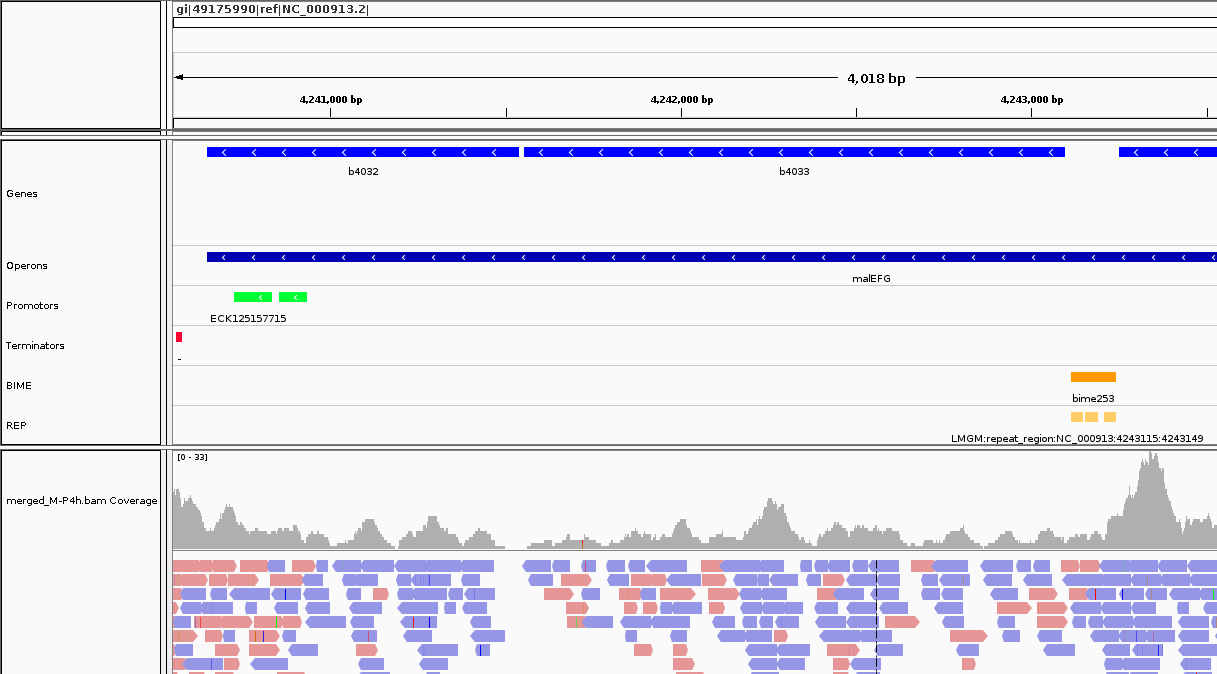
\includegraphics[scale=0.3]{figures/igv_snapshot.png}
\caption{\textbf{Visualisation du mapping de l'opéron malEFG sur IGV.} Les premières pistes représentent les positions et orientations des gènes, des opérons, des promoteurs, des terminateurs, des BIME et des REP. Les 2 pistes suivantes affichent la couverture de la région visualisée (histogramme gris) et l'alignement des reads (flèches pleines rouges et bleues). La couleur bleue sur cette piste indique un alignement sur le brin direct et la couleur rouge sur le brin complémentaire.}
\label{fig:igv}}
\end{SCfigure}

\section*{Création de la table de comptages et normalisation}
Afin d'obtenir des résultats de comptage par région d'intérêt et ainsi estimer l'expression, nous avons utilisé le package Bioconductor easyRNASeq \citep{Delhomme2012} puisqu'il permet de réaliser les opérations de comptage de façon documentée et qu'il offre la possibilité d'effectuer une normalisation. Les annotations du génome d'\textit{E. coli} relatives aux gènes sont extraites à partir du fichier \texttt{GFF} et stockées sous forme d'une base de données.
La liste des transcrits par gène est ensuite extraite pour un total de 4605 éléments que nous nommerons régions. La couverture par région est ensuite calculée pour chaque fichier \texttt{BAM}, le résultat est obtenu en réalisant l'union des positions extraites de la liste des régions et des positions des reads extraites des fichiers BAM qui auront été préalablement transformées au format \gls{GRanges} (\texttt{GRanges})  \citep{Lawrence2013}. Une table de comptage est alors produite, les régions figurant en ligne et les fichiers BAM en colonnes.

Les résultats de comptages doivent ensuite être normalisés afin de permettre la comparaison de l'expression des gènes et des régions génomiques d'intérêt. De nombreuses méthodes de normalisation existent basées sur différents concepts, l'ajustement de la distribution des comptes des reads et la taille de la librairie. Sur les méthodes du premier concept, certaines sont basées sur les quantiles (Upper Quartile, Mediane, Quantile) ou prennent en compte la taille du transcrit par rapport au nombre de reads de la bibliothèque (\gls{rpkm}). Cette dernière méthode de normalisation est soumise à critique à juste titre \citep{Dillies2013} car elle induit un biais de lors d'une analyse de \gls{de} dans le cas de gènes fortement exprimés dans un condition par rapport aux autres conditions. Comme nous ne nous situons pas dans le cadre d'une analyse différentielle sur plusieurs conditions, mais que nous comparons des réplicats d'une même condition, nous pouvons appliquer cette normalisation. Notre choix s'est donc porté sur cette méthode \citep{Mortazavi2008} :

\[RPKM = Nb.~reads~transcrit~*~\frac{10^9~bases}{Nb.~total~reads~*~Taille~du~transcrit}\]

Il faut souligner que comme nous ne nous intéressons pas à un même gène dans 2 conditions différentes mais à 2 gènes dans une même condition, un biais dû à leur composition en GC peut intervenir. Le déroulé de l'analyse pour produire la table de comptage normalisée est présenté sur la \autoref{fig:data_preparation}.

\section*{Détermination des transcrits}
\label{methode_correlation}
Le principe de cette analyse repose sur la recherche de corrélation entre le profil d'expression issu de données de RNA-Seq et un profil théorique représentant un changement de niveau d'expression, cette méthode a été mise au point pour la prédiction d'opérons dans les génomes bactériens \citep{Fortino2014}. Le principe général est de délimiter les bornes des transcrits à partir de données de couverture en s'appuyant sur un test de corrélation entre ce profil et un profil arbitraire de 0 et de 1. Les 0 représentant une zone sans couverture donc en dehors d'un transcrit et les 1 la zone couverte, donc le transcrit. Le cœur de leur méthode consiste à déplacer une fenêtre glissante de 100 pb parcourant base à base le génome en réalisant des tests de corrélation entre le profil d'expression réel et le profil d'expression simulé par le vecteur de même taille contenant un nombre égal de 0 et de 1 (dans le cas d'une croissance du niveau d'expression sur le brin direct ou une décroissance du niveau d'expression sur le brin complémentaire, \textit{e.g}: 000111), ou de 1 et de 0 (dans le cas dans le cas d'une décroissance du niveau d'expression sur le brin direct ou une croissance du niveau d'expression sur le brin complémentaire, \textit{e.g}: 111000). Les moyennes du taux de couverture sont calculées sur les parties gauche et droite de la fenêtre pour dans un premier temps filtrer les données, le $Log_2$ du rapport de ces moyennes doit être supérieur à 1 ce qui représente un changement de 2 fois du niveau d'expression. Si ce 1\up{er} filtre est passé, la corrélation entre le profil réel et celui simulé est calculée et doit être supérieure à un seuil avec une p-valeur significative du test de corrélation pour être validée (\autoref{fig:profil}). Les auteurs ont fixé un seuil minimum de corrélation de 0.7 et une p-valeur de $10^{-7}$ comme seuil significatif pour le test de corrélation.

\begin{SCfigure}[][h!]
\fbox{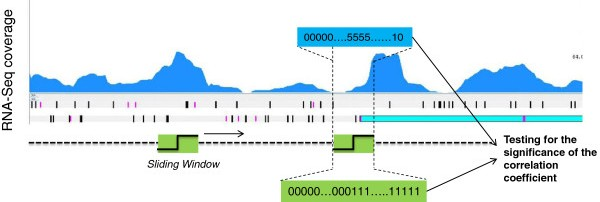
\includegraphics[scale=0.6]{figures/profil.jpg}
\caption{\textbf{Recherche de corrélation sur des profils d'expression.} La fenêtre glissante (en vert) parcourt la région d'intérêt et pour chaque déplacement une corrélation est calculée entre le vecteur du profil d'expression obtenu par RNAseq (en bleu) et celui simulé par le vecteur de 0 et de 1 (en vert) \citep{Fortino2014}.
\label{fig:profil}}}
\end{SCfigure}

\section*{Segmentation}
\label{methode_segmentation}
A la différence de la méthode précédente, la segmentation ne requière pas l'utilisation de profils. La méthode de segmentation que nous utilisons est issue du package R \href{http://cran.r-project.org/web/packages/Segmentor3IsBack/index.html}{Segmentor3IsBack} \citep{Cleynen2014}. Le but de cette méthode est de rechercher, sur une zone d'intérêt, des points de changements abrupts dans la couverture en utilisant l'algorithme \gls{pdp} \citep{Rigaill2010}. La segmentation se fonde sur le partitionnement d'un signal de $n$ points, la couverture de notre région d'intérêt, compris dans l'ensemble ${\{y_t\}_{t=1,\ldots,n}}$, suivant une distribution de Poisson, en $K$ segments, tel que :
\[ Y_t \sim G(\theta_r) \quad \text{si}\ t \in r \quad \text{et}\ r \in m \]
où $m$ est une partition de $[1,n]$ en $r$ segments, le paramètre $\theta_r$ est la moyenne associée au segment $r$. L'objectif étant d'estimer la position des segments et le paramètre $\theta_r$ résultant de la segmentation. $M_{K,n}$ est alors l'ensemble des partitions possibles avec $K$ le nombre maximal de partitions demandé et $n$ la taille de notre région. L'algorithme tente de choisir la partition $M_{K,n}$ avec la perte $\gamma$ minimale. Cette perte est calculée par la négative log-likelihood du modèle. La fonction de calcul du coût est définie comme telle :
\[ c(r,\theta) = \sum_{i \in r} \gamma(y_i,\theta) \]
et dont le coût optimal sera :
\[ c(r) = min_\theta\{c(r,\theta)\} \]
cela permettant de déterminer la segmentation optimale $M_{K,n}$ et son coût $C_{K,n}$. L'algorithme itératif PDP intervient ensuite et est basé sur la minimisation de la fonction de coût $C_{k,t}$ décomposée de la façon suivante :
\begin{equation}
\label{eq1}
C_{k,t} = \underset{\{k-1<\tau<t\}}{min} \{C_{k-1,\tau} + \underset{\theta}{min}[c([\tau + 1,t],\theta)]\}
\end{equation}
où $\theta$ est le paramètre de coût du dernier segment directement lié au calcul de perte $\gamma$. La spécificité de cet algorithme est qu'il s'appuie sur la comparaison de candidats pour la position du dernier point de cassure notée $\tau$ à travers les permutations des minimisations de \eqref{eq1} et avec l'introduction de la fonction :
\[ H_{k,t}(\theta) = \underset{\{k-1<\tau<t\}}{min} \{C_{k-1,\tau} + c([\tau + 1,t],\theta)\} \]
qui est le coût de la meilleure partition en $k$ régions jusqu'à $t$, le paramètre du dernier segment étant $\theta$. $C_{k,t}$ est alors obtenu comme le $min_\theta\{H_{k,t}(\theta)\}$.
Pour chaque itération $k$, l'algorithme travaille sur une liste de candidats pour les derniers points de cassure. Pour chaque élément $\tau$ et chaque valeur $t$, il met à jour un ensemble $S_{k,t}^\tau$ contenant les paramètres $\theta$ pour lequel ce candidat est optimal. Si cet ensemble $S_{k,t}^\tau$ est vide, le candidat est supprimé autorisant un élagage et une diminution de la complexité de l'algorithme.

Au final, l'utilisation de ce package produit un découpage de la région d'intérêt en $K$ segments, $K$ étant fixé par l'utilisateur, dont les limites sont définies par les positions de leurs points de cassures.

\section*{Reconstruction des séquences ancêtres et structures secondaires}
En pratique, nous disposons de l’annotation des REP dans un ensemble de 86 génomes complets d’\textit{Escherichia} et \textit{Shigella}. Cette annotation est complétée par l’identification des loci contenant des REP orthologues \citep{Weyder2013}. Ainsi, pour les paires de gènes contenant une BIME dans leur RIG chez \textit{E. coli K12 MG1655}, nous pouvons connaître, pour tous les autres génomes complets  d’\textit{Escherichia} et \textit{Shigella}, l’état de la RIG vis-à-vis de la BIME des gènes orthologues correspondant : présence ou absence d’une BIME et en cas de présence composition en REP de la BIME. 
La reconstruction des séquences ancêtres nécessite un arbre modèle pour l’évolution des espèces/souches de bactéries considérées. Cet arbre a été inféré à l’aide d’une sélection de  583 gènes orthologues conservés dans ces génomes. Les alignements multiples de ces familles de gènes sont concaténés et une méthode de maximum de vraisemblance (\texttt{PhyML}) a été utilisée pour calculer l’arbre phylogénétique \citep{Weyder2013}. A l’aide de cet arbre et de la séquence des BIME au niveau des loci orthologues (feuilles de l’arbre), il est possible d’inférer les séquences ancêtre à chaque nœud de l’arbre. Plusieurs méthodes sont disponibles \citep{Bosc2014}. Nous avons choisi une méthode de maximum de vraisemblance implémentée dans le logiciel \texttt{PHAST} \citep{Hubisz2011}. L'objectif de la méthode du maximum de vraisemblance est d’inférer les états ancêtres aux nœuds (le type de nucléotide dans notre cas) d'un arbre afin de rendre l'arbre reconstruit le plus vraisemblable étant donné les données aux feuilles de l'arbre et le modèle d'évolution \citep{Pagel1999}. Le maximum de vraisemblance repose sur un modèle d’évolution et permet de prendre en compte la longueur des branches et permet de multiples changements le long d'une seule branche. Nous avons utilisé le modèle HKY85 qui prend en compte des taux de transition et de transversion différents. 
La prédiction des structures secondaires a été réalisée à l’aide du package R \texttt{ViennaRNA} \citep{Lorenz2011}. L’énergie libre minium des structures a été calculée avec le programme \texttt{RNAfold}  pour les séquences uniques (réelles ou inférées) et avec le programme \texttt{RNAalifold} pour les alignements de BIME orthologues. 

\chapter*{Résultats}

Pour réaliser les analyses, nous nous sommes inspirés de la méthodologie employée en RNA-Seq pour l'étude de DE. L'analyse statistique de recherche de changement d'expression liée à la présence de BIME a été menée sur le logiciel R. La première étape a consisté à examiner les données d'expression concernant les gènes des opérons dans les cas où ils flanquent une BIME ou non, en partant de l'hypothèse que les gènes d'un même opéron ont un profil d'expression similaire en absence d'\gls{et} tels que les promoteurs et les terminateurs de transcription. Nous avons ensuite recherché des changements de niveaux d'expression qui pourraient être liés à la présence de BIME dans la \gls{rig} de deux gènes d'un opéron par une approche locale (la corrélation de profils d'expression) et une approche de segmentation. Nous avons reconstruit les séquences ancêtres et étudiés les structures secondaires des BIME détectées par les trois méthodes à la fois. Cette chaîne de traitement permettra facilement d'étendre l'étude à d'autres jeux de données.

Dans un souci de simplification de la notation, nous nommerons gène 1, le gène en amont de la BIME dans le sens de la transcription et gène 2 celui en aval.

\section*{Couverture du génome}
\label{uniformite_couverture}
Un des problèmes majeur de ce type d'approche est que la couverture des reads le long du génome n'est pas uniforme (\autoref{fig:igv}), ceci peut s'expliquer par différentes raisons techniques \citep{Li2013}. Premièrement, les \textbf{méthodes de fragmentation} des protocoles de préparation des bibliothèques amènent un biais en cassant ou dégradant certaines séquences. Le second biais possible est produit par le \textbf{Random Priming} lors de l'étape de rétro-transcription pouvant préférentiellement transcrire certaines séquences. Troisième point, les \textbf{ligases peuvent lier préférentiellement les adaptateurs} à certaines séquences. Quatrième point, l'amplification de la PCR est bien connue pour introduire des \textbf{biais dépendant de la proportion en GC} des séquences (formation de structures secondaires et température de dénaturation plus élevée). Le dernier point particulier au séquençage Illumina implique, lors du processus d'élongation du séquençage, des \textbf{interférences spécifiques aux séquences} générées par des schémas particuliers du template, tels que des répétitions de GCC ou CGG et des répétitions inversées d'une séquence de plus de 8 pb sur un même brin (\textit{e.g} : \textcolor{blue}{AAAAAACCTTGAAAAGCC}\textcolor{cyan}{A}\textcolor{blue}{GGCTTTTCAAGGTTTTTTT}), produisant des repliements du brin d'ADN et altérant l'affinité des enzymes \citep{Nakamura2011}. 

Les données provenant de la technologie Illumina et les REP étant des séquences répétées inversées mais contenant des sites de mésappariement, elles sont susceptibles de subir ce biais et nous risquons d'obtenir des valeurs de couverture erronées sur ces éléments. Pour cela, nous nous sommes intéressés aux RIG contenant des BIME mais pas de promoteurs et de terminateurs, pour lesquelles aucun changement significatif de taux de transcription n'est observé entre les gènes amont et aval. Les  différences de niveaux d'expression entre les deux gènes pour les trois jeux de données ont été contrôlées à l'aide d'un test de rang de Wilcoxon pour vérifier l'égalité des médianes (p-valeur < 0.01). Pour toutes les paires de gènes dont le niveau d'expression n'est pas différentié, nous avons vérifié l'expression du gène amont par rapport à celle de la BIME (\autoref{fig:same_expression_operon_point}).

\begin{SCfigure}[][h!]
\fbox{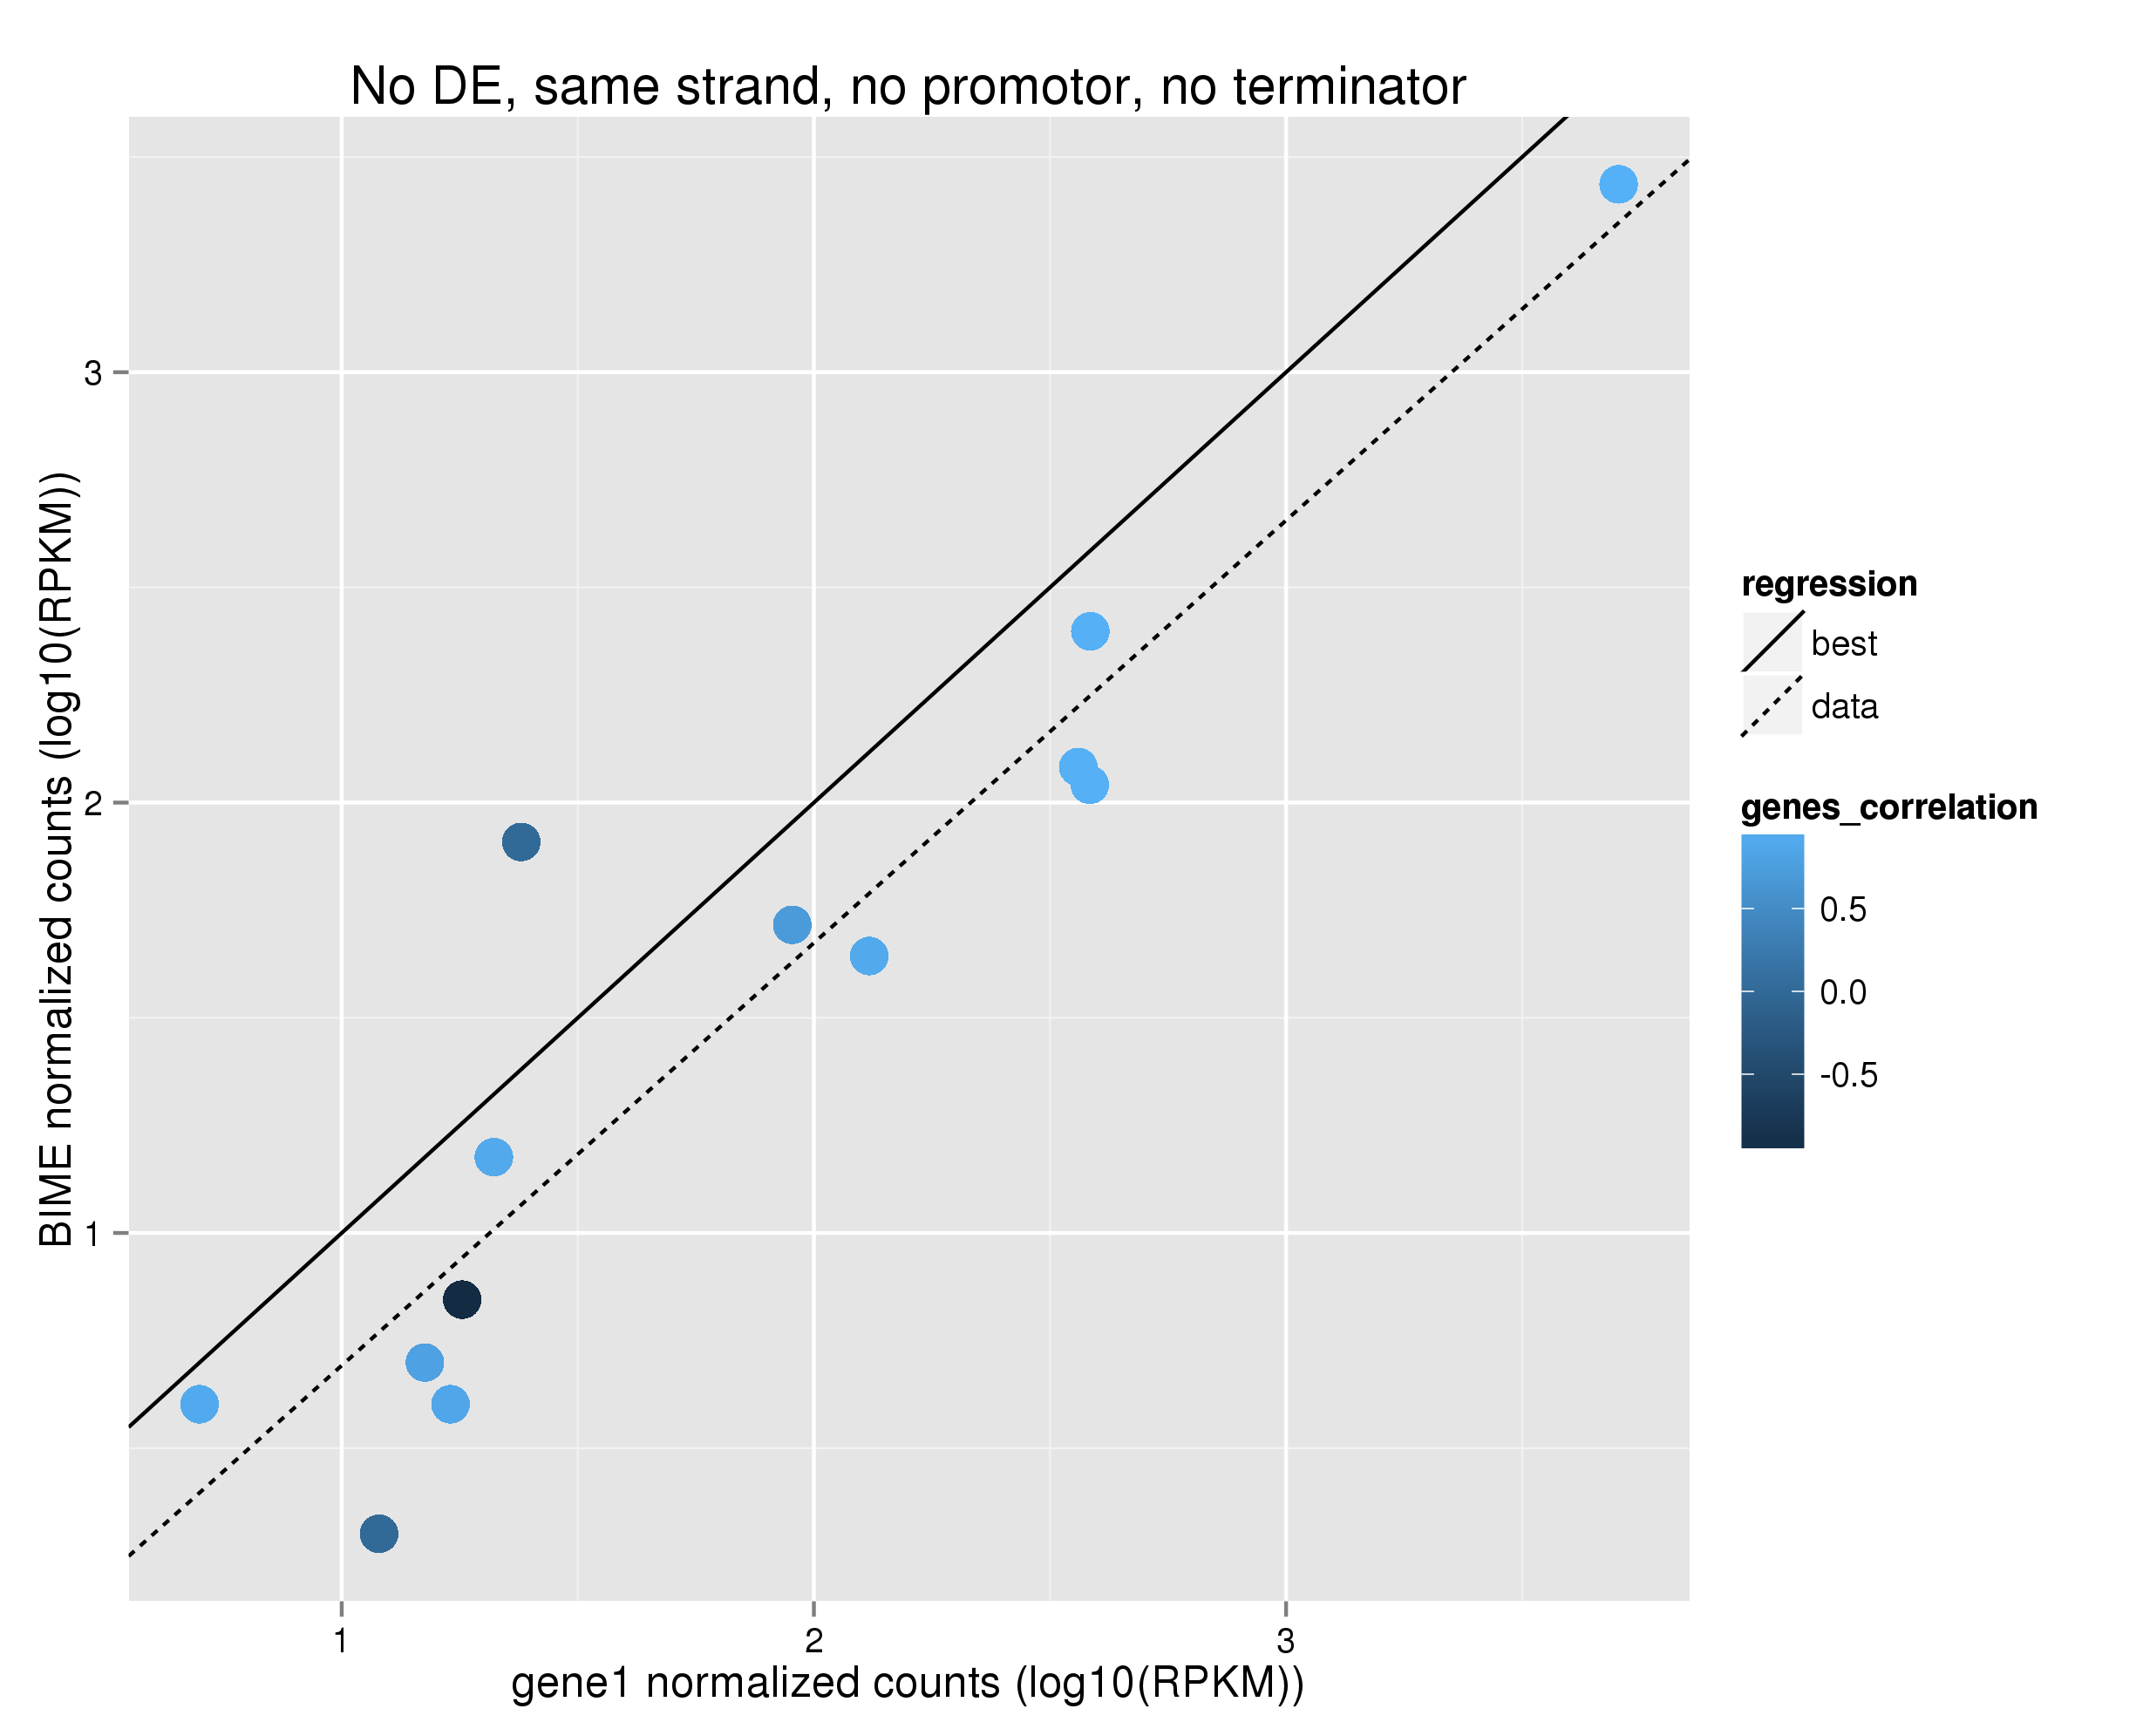
\includegraphics[scale=0.5]{figures/scatterplotSameStrandNoReg_all.png}
\caption{\textbf{Niveau d'expression de la BIME par rapport aux gènes flanquant non DE dans les opérons en absence de promoteurs et de terminateurs de transcription.} Les 3 jeux de données sont représentés ici. L'axe des abscisses représente le niveau d'expression du gène 1 en $log_{10}$, celui des ordonnées le niveau d'expression de la BIME en $log_{10}$. La coloration des points représente la corrélation du niveau d'expression du premier gène par rapport au second gène flanquant la BIME. La droite pleine représente la régression dans le cas où l'on observe une régression linéaire idéale, celle en pointillés représente la régression sur les valeurs des 3 jeux de données.
\label{fig:same_expression_operon_point}}}
\end{SCfigure}

Nous observons une corrélation linéaire entre le taux d'expression du gène 1 et celui de la BIME (coefficient de corrélation : 1.037). Cependant, si la droite de régression possède un pente proche de 1, elle est décalée vers la droite par rapport à celle simulant un taux d'expression entre le gène 1 et la BIME. Ce résultat montre un biais systématique des données de RNA-Seq des échantillons testés vers une sous-estimation du taux d'expression des BIME. Nous baserons donc l'étude globale de l'effet des BIME sur le différentiel d'expression entre les gènes les flanquant.

\section*{BIME et unités de transcription}
Chez \textit{E. coli K12}, sur les 848 opérons formés de plus d'un gène, 36 contiennent au moins une BIME et comme un opéron peut contenir plusieurs BIME un total de 39 BIME sont présentes entre deux gènes. Nous nous sommes intéressés à ces opérons multigéniques afin d'étudier les caractéristiques de ceux contenant des BIME et comparer l'expression des gènes consécutifs des opérons en présence et absence de BIME. La distribution du nombre de gènes par opérons est répertoriée figure \autoref{fig:operonFigA}, les opérons ne contenant que deux gènes sont les plus représentés (51\%) et l'opéron le plus grand contient 16 gènes. Les opérons de 3 gènes (21\%) sont ceux qui contiennent le plus souvent une BIME.

\begin{figure}[h!]
\centering
\subfigure[]{\label{fig:operonFigA} 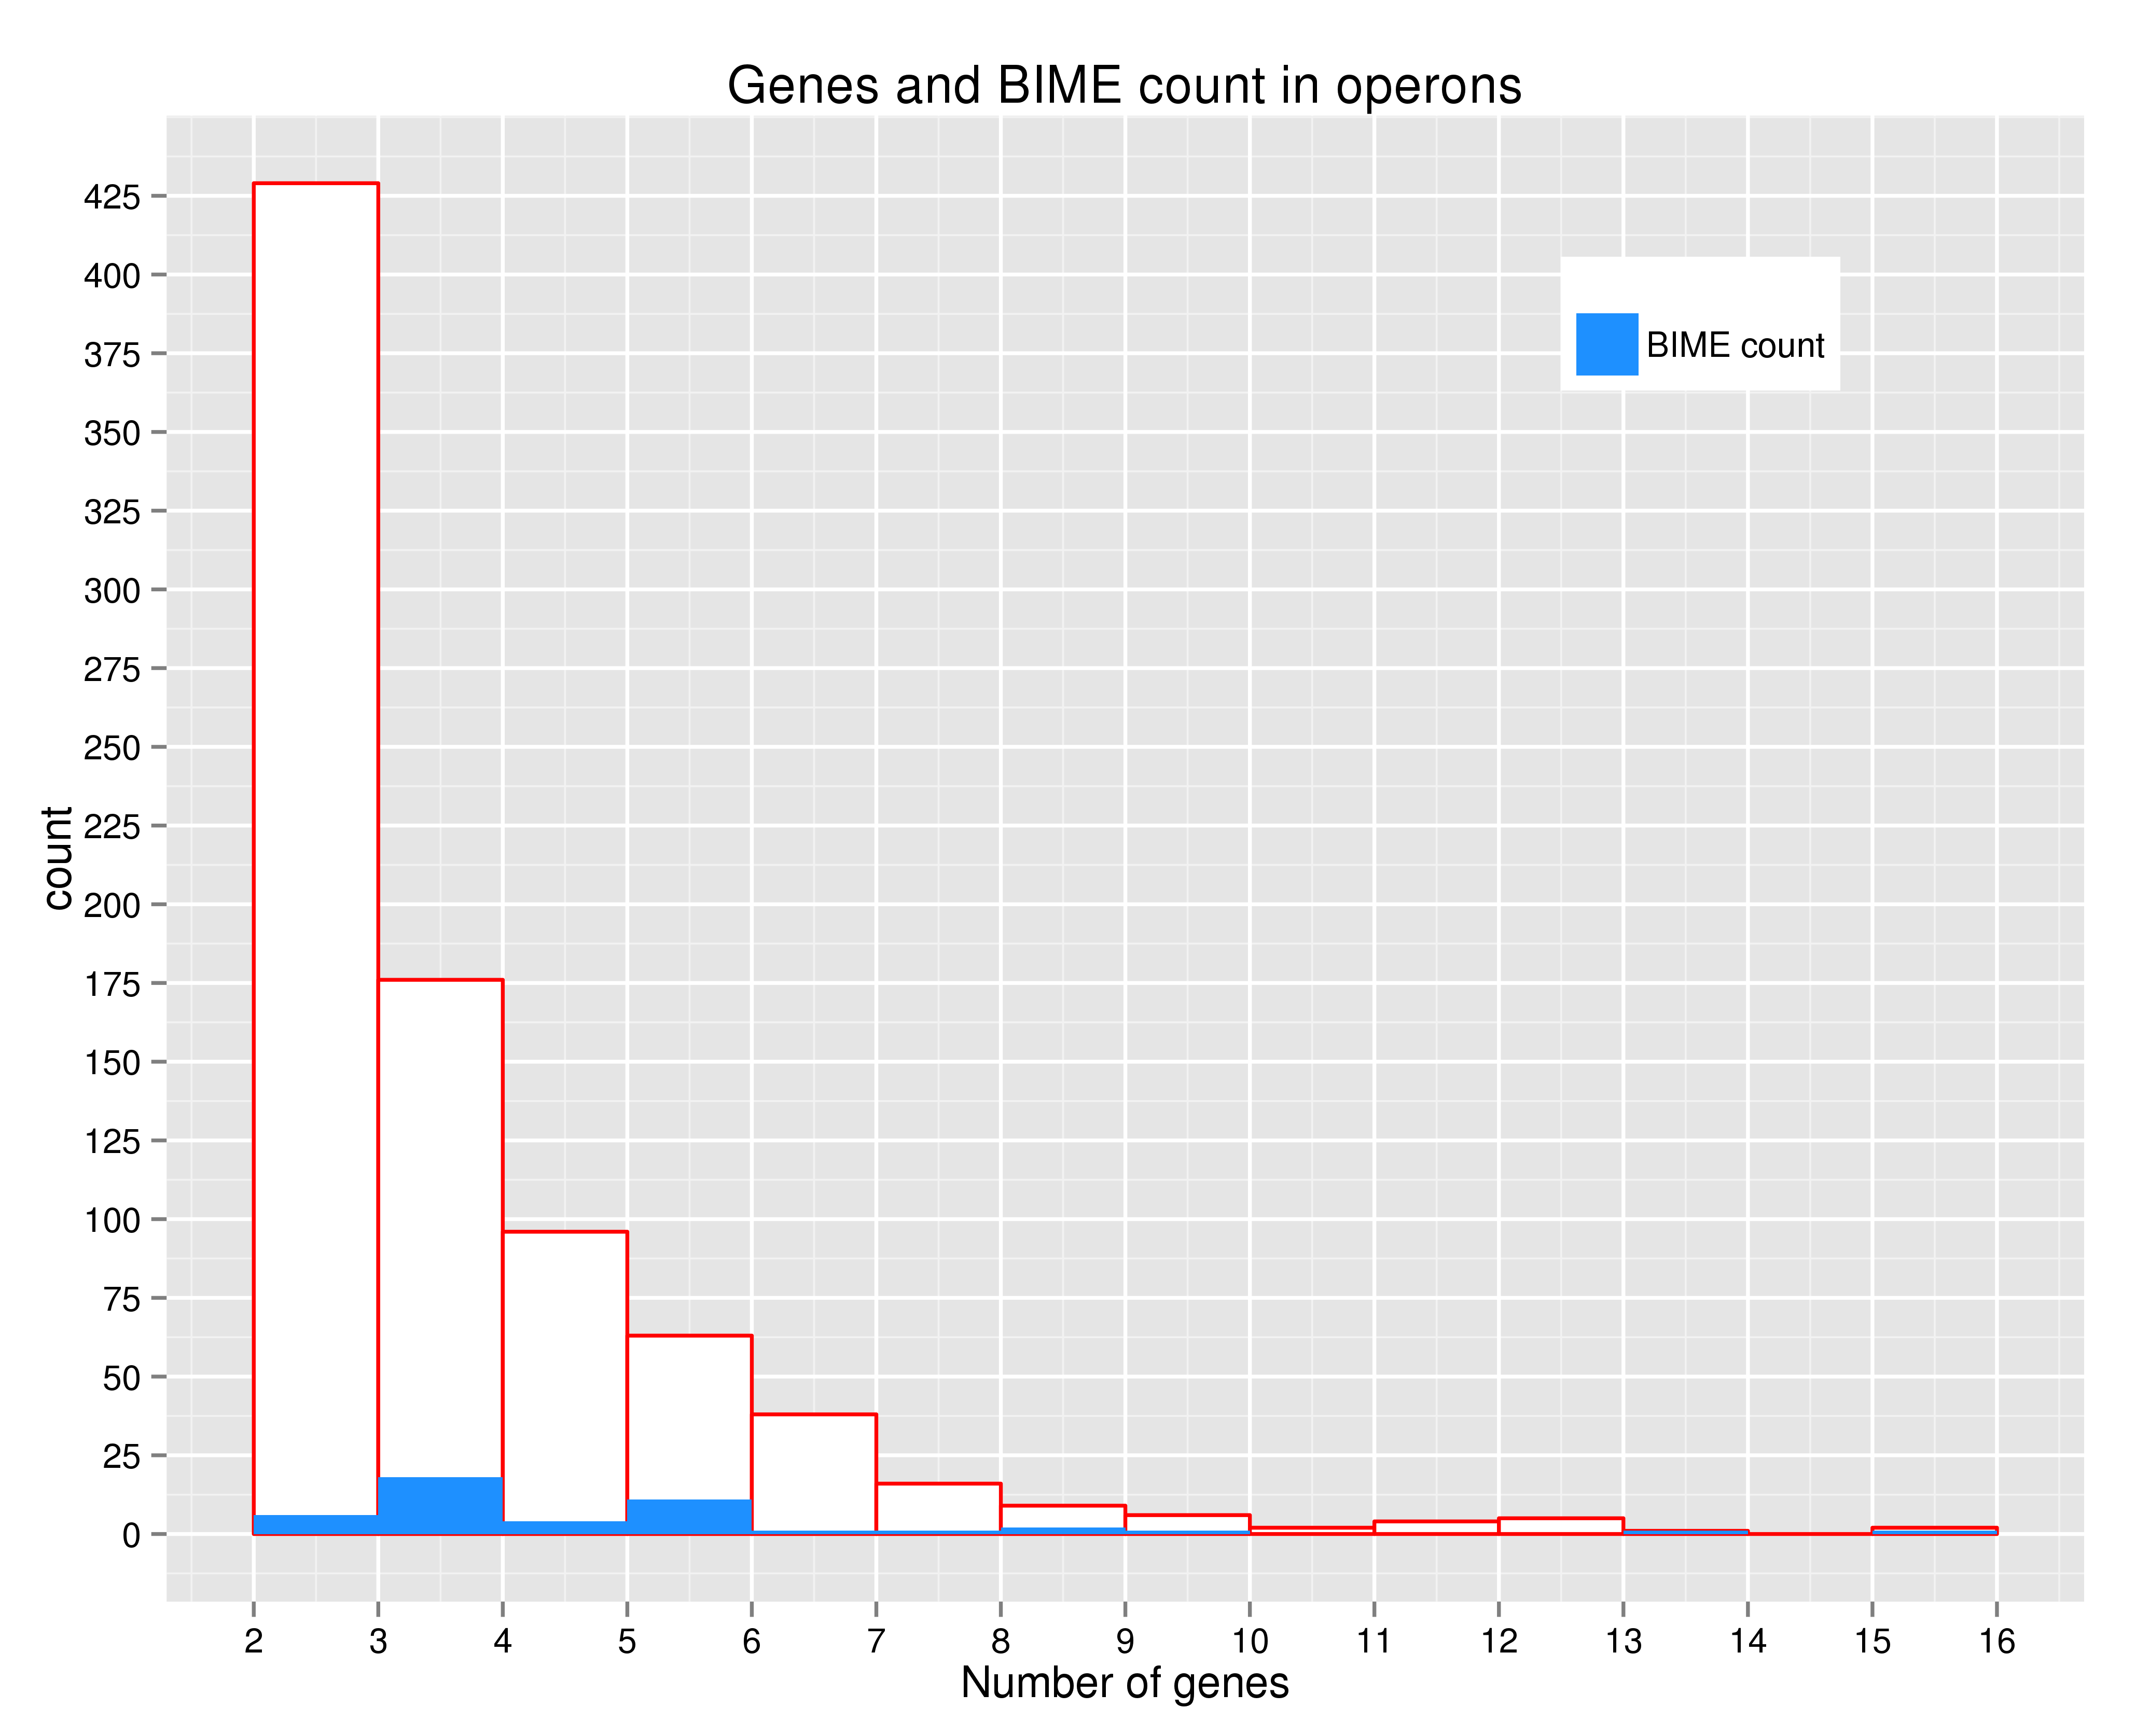
\includegraphics[scale=0.38]{figures/nbGenesBimeByOperon.png}}
\subfigure[]{\label{fig:operonFigB} 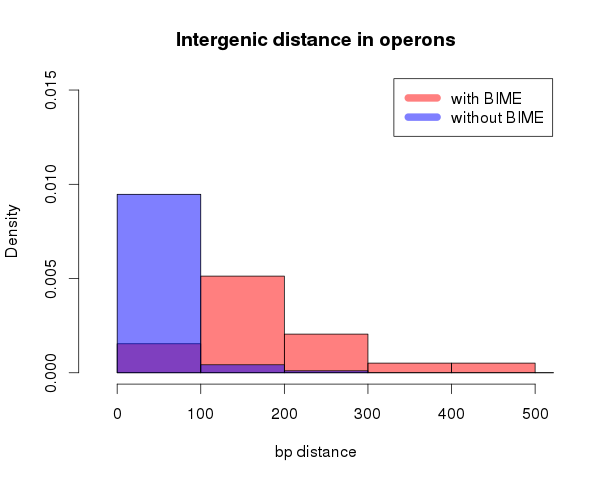
\includegraphics[scale=0.38]{figures/igr_distance.png}}
\subfigure[]{\label{fig:operonFigC} 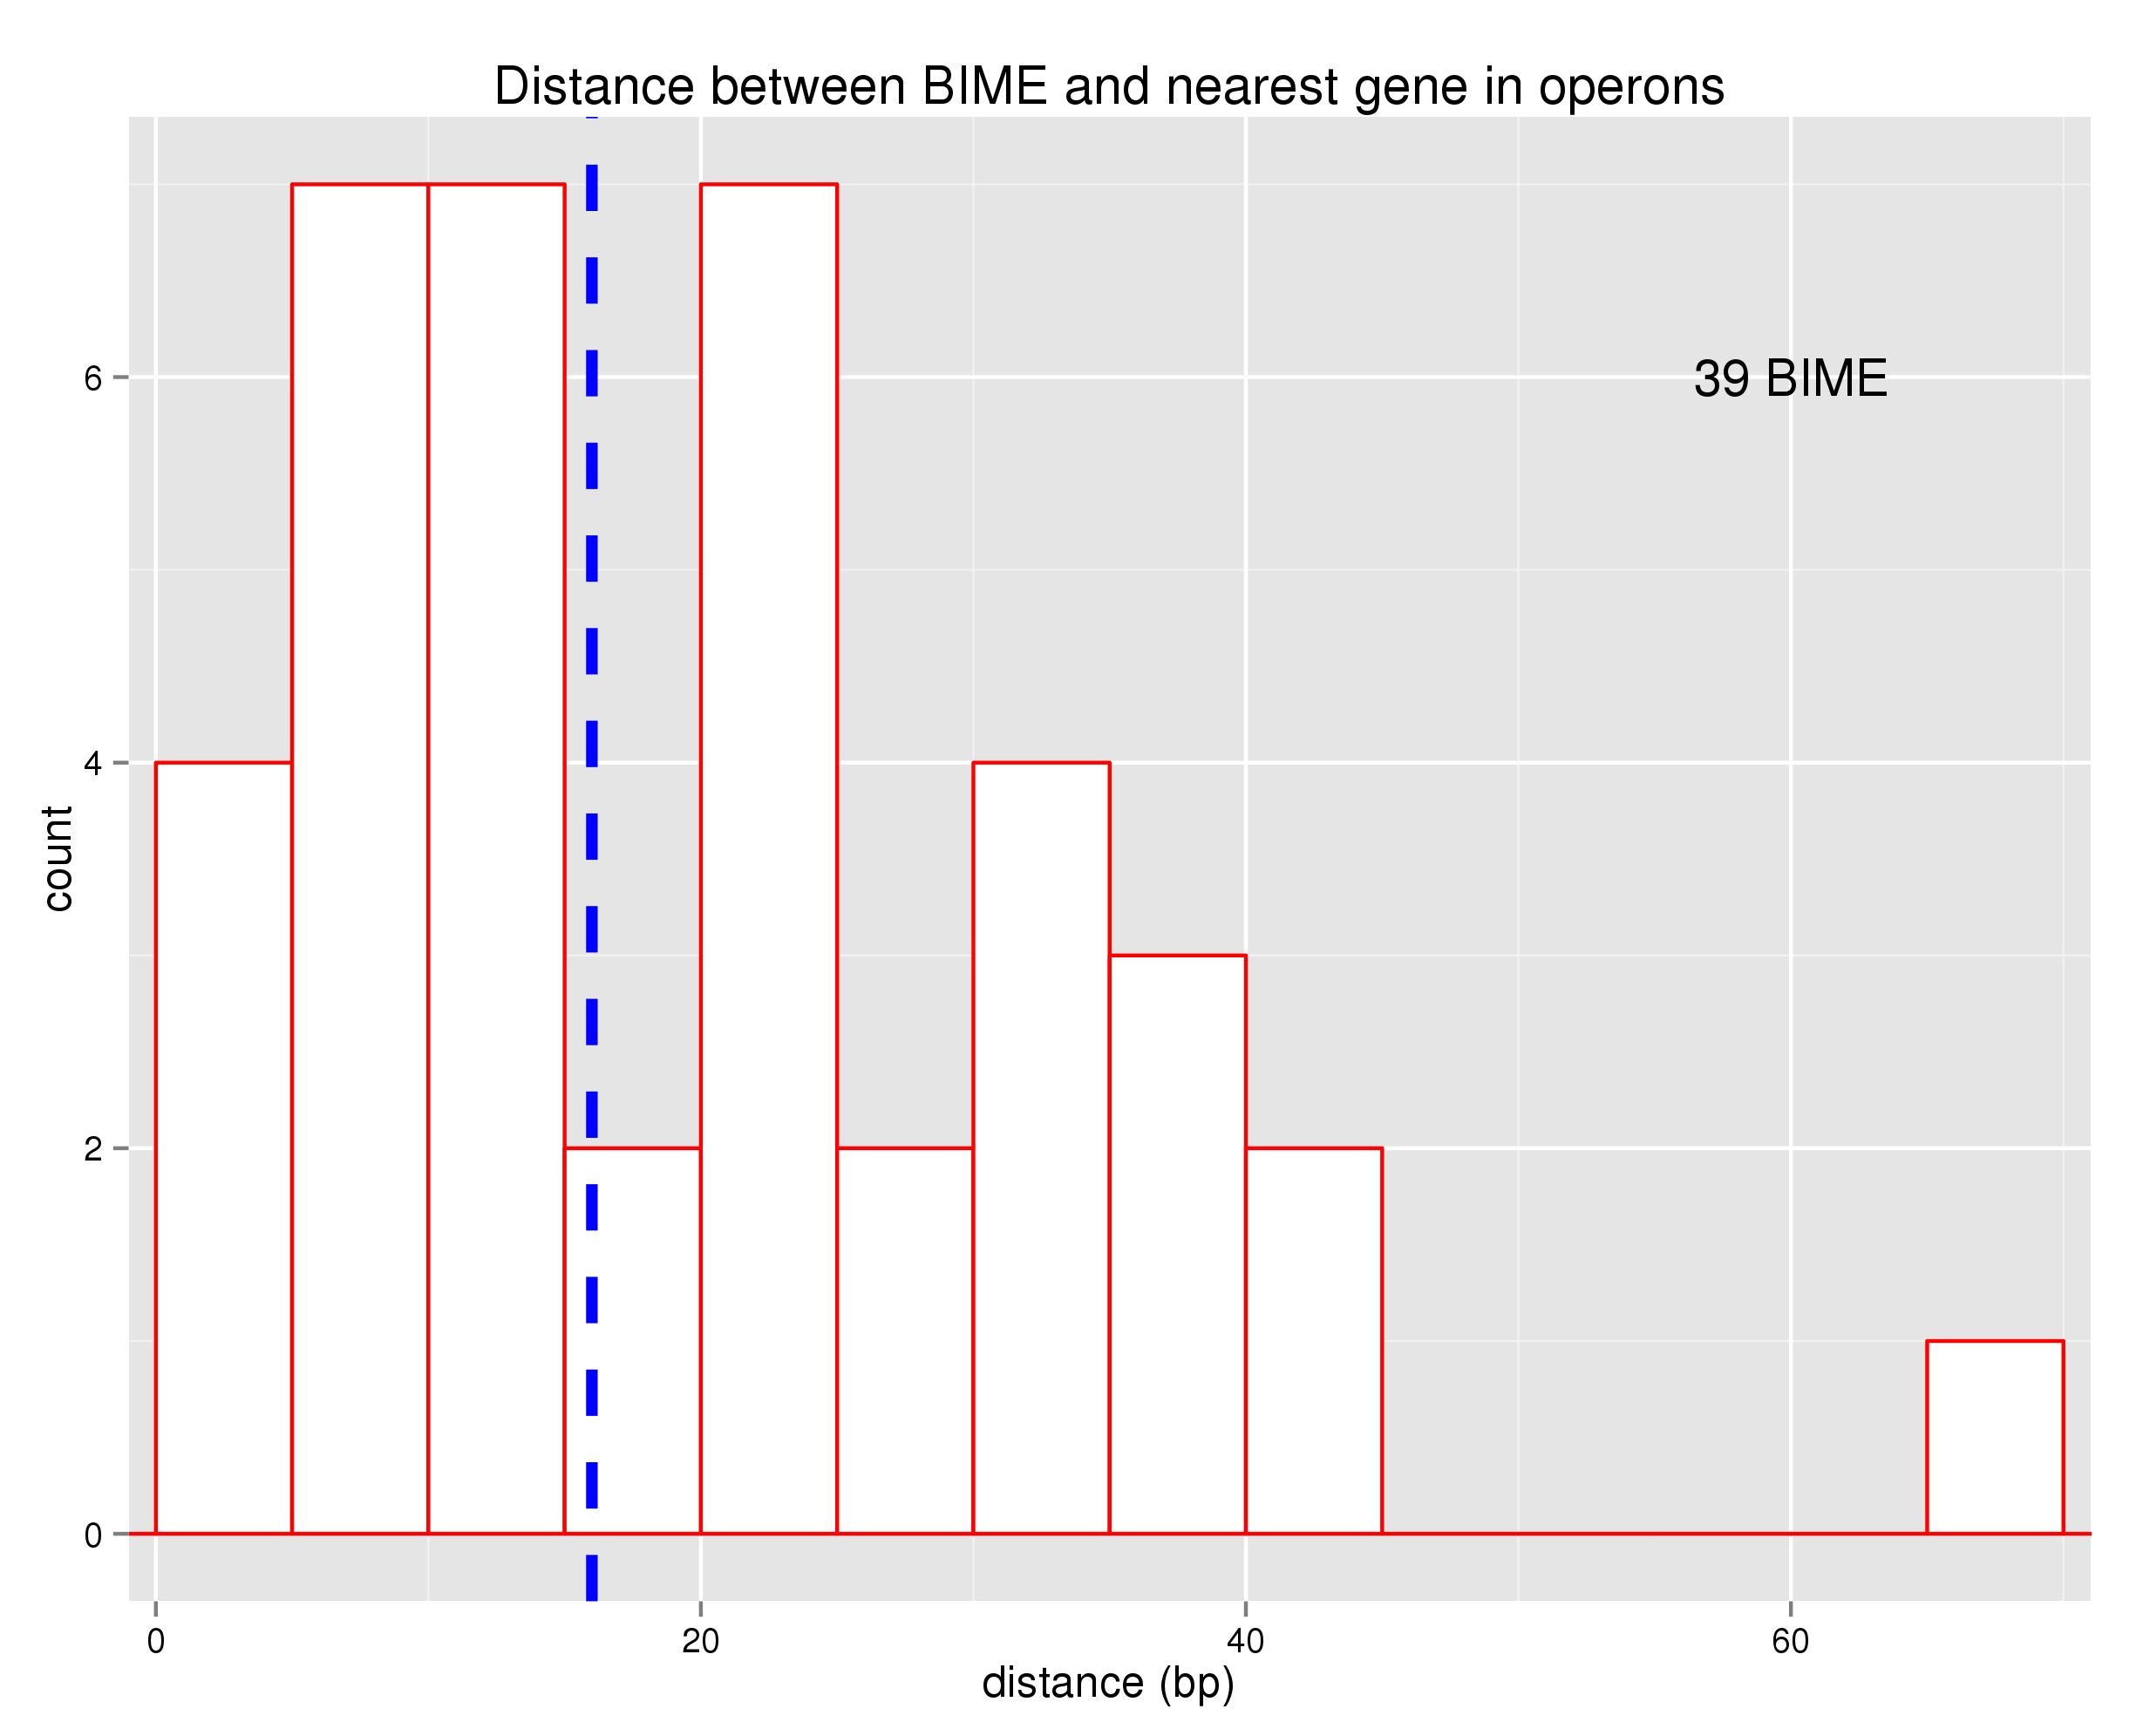
\includegraphics[scale=0.38]{figures/distance_BIME_gene_in_operon.png}}
\caption{\textbf{(a) Distribution du nombre de gènes par opérons et répartition des BIME.} L'échelle des abscisses indique le nombre de gènes dans l'opéron. Les histogrammes blancs représentent le compte du nombre d'opérons, les histogrammes bleus le compte des BIME au sein des opérons. La grande majorité des opérons sont constitués de 2 gènes mais peuvent aller jusqu'à 16 gènes. Sur les 36 BIME présentes dans les opérons, 18 sont dans des opérons de 3 gènes, 11 dans ceux de 5 gènes et 6 dans ceux de 2 gènes. \textbf{(b) Distances inter-géniques dans les opérons avec et sans BIME.} L'échelle des ordonnées représente la densité car l'écart entre les valeurs avec ou sans BIME est trop important pour une visualisation correcte de l'histogramme avec les effectifs. En bleu absence de BIME dans la RIG, en rouge présence de BIME. Pour les données en absence de BIME, nous observons une valeur modale dans les régions inter-géniques de 50 pb, alors qu'en présence de BIME, la valeur modale se situe dans les régions inter-géniques de 150 pb. \textbf{(c) Distance de la BIME au gène le plus proche dans les opérons.} En ordonnées le nombre de BIME, en abscisses la distance de la BIME au gène le plus proche pour les 39 BIME situées dans les opérons. La ligne pointillé bleue représente la médiane des distances située à 16 pb.
\label{fig:operon}}
\end{figure}

Une des conséquences directe de la présence d'une BIME dans une RIG est une augmentation significative de la distance inter-génique (Figure \autoref{fig:operonFigB}), la taille médiane sans BIME est de 8 pb et passe à 162 pb en leur présence. Cet allongement de la RIG peut avoir des conséquences sur la stabilité de l'ARNm polycistronique. En effet, cette région n'étant pas couverte par les ribosomes en cours de traduction, elle sera plus exposée aux attaques d'une endoribonucléase. Néanmoins, cet effet peut être compensé par la formation d'une structure secondaire stable par la séquence de la BIME pouvant inhiber l'action des endoribonucléases. Notons que l'allongement de la RIG due à la présence d'une BIME peut conduire à l'échec des méthodes de prédiction des opérons qui utilisent entre autre le critère de taille de la RIG dans leurs calculs. Il est donc possible que le nombre de BIME dans les opérons soit sous-estimé dans RegulonDB.

La localisation de la BIME par rapport au codon d’initiation ou stop des gènes peut également affecter la transcription et la traduction de ce gène.  Nous avons reporté cette distribution figure \autoref{fig:operonFigC}. Il apparaît clairement que les BIME sont plus proche du codon stop du gène 1 que du codon d’initiation du gène aval. En effet, il a été montré qu’une trop grande proximité de la BIME avec le codon stop peut conduire à un blocage au moins partiel du ribosome pouvant conduire à un arrêt prématuré de la traduction pouvant aller jusqu’à la dégradation de la protéine et même du messager par la RNase R \textcolor{red}{(ref)}. Ce mécanisme de régulation pourrait être à l’œuvre pour \textcolor{red}{le gène xxx}, mais il semble assez contre-productif pour être généralisé \textcolor{red}{(ref)}. D’autre part, une trop grande proximité avec le codon initiateur pourrait masquer la séquence Shine-Dalgarno ou ce codon dans la structure secondaire formée par la BIME et ainsi affecter l’initiation de la traduction du gène.

\section*{Effet global dans les unités de transcription}
Dans un premier temps, nous avons voulu étudier globalement l'effet des BIME sur le taux de transcription des gènes la flanquant. Comme référence, nous avons utilisé les paires de gènes consécutifs qui appartiennent aux même opéron mais qui ne sont pas séparés par une BIME. Comme nous l'avons évoqué plus haut, l'analyse peut être affectée par la présence de promoteurs ou de terminateurs de transcription. D'autre part la taille des RIG peut également influencer la stabilité des messagers même en l'absence de BIME. En raison du faible effectif de RIG contenant des BIME, nous avons été contraints dans un premier temps de regrouper les promoteurs et terminateurs dans une seule classe et de faire deux classes de tailles de RIG. Un seuil de 150 pb, proche de la médiane des RIG avec BIME a été fixé pour équilibrer les effectifs.

Les taux d'expression des gènes consécutifs d'un opéron, en absence de BIME et d'ET, présentent une forte corrélation linéaire mais sur un intervalle de valeurs étendu. Afin de comparer les écarts entre taux d'expression des gènes, nous avons utilisé un indice, $I_{expr}$, qui pondère la différence observée par la somme des taux d'expression des deux gènes :

\[ I_{expr} = \frac{RPKM_{gene2} - RPKM_{gene1}}{RPKM_{gene2} + RPKM_{gene1}} \quad I_{expr} \in [-1,1]\]

Nous mesurons ainsi un biais sur l'intervalle [-1,1] et qui est égal à 0 si aucune différence est observée, qui devient négatif dans le cas d'un taux d'expression plus important du gène 1 et positif dans le cas inverse.

\begin{figure}[h!]
\centerline{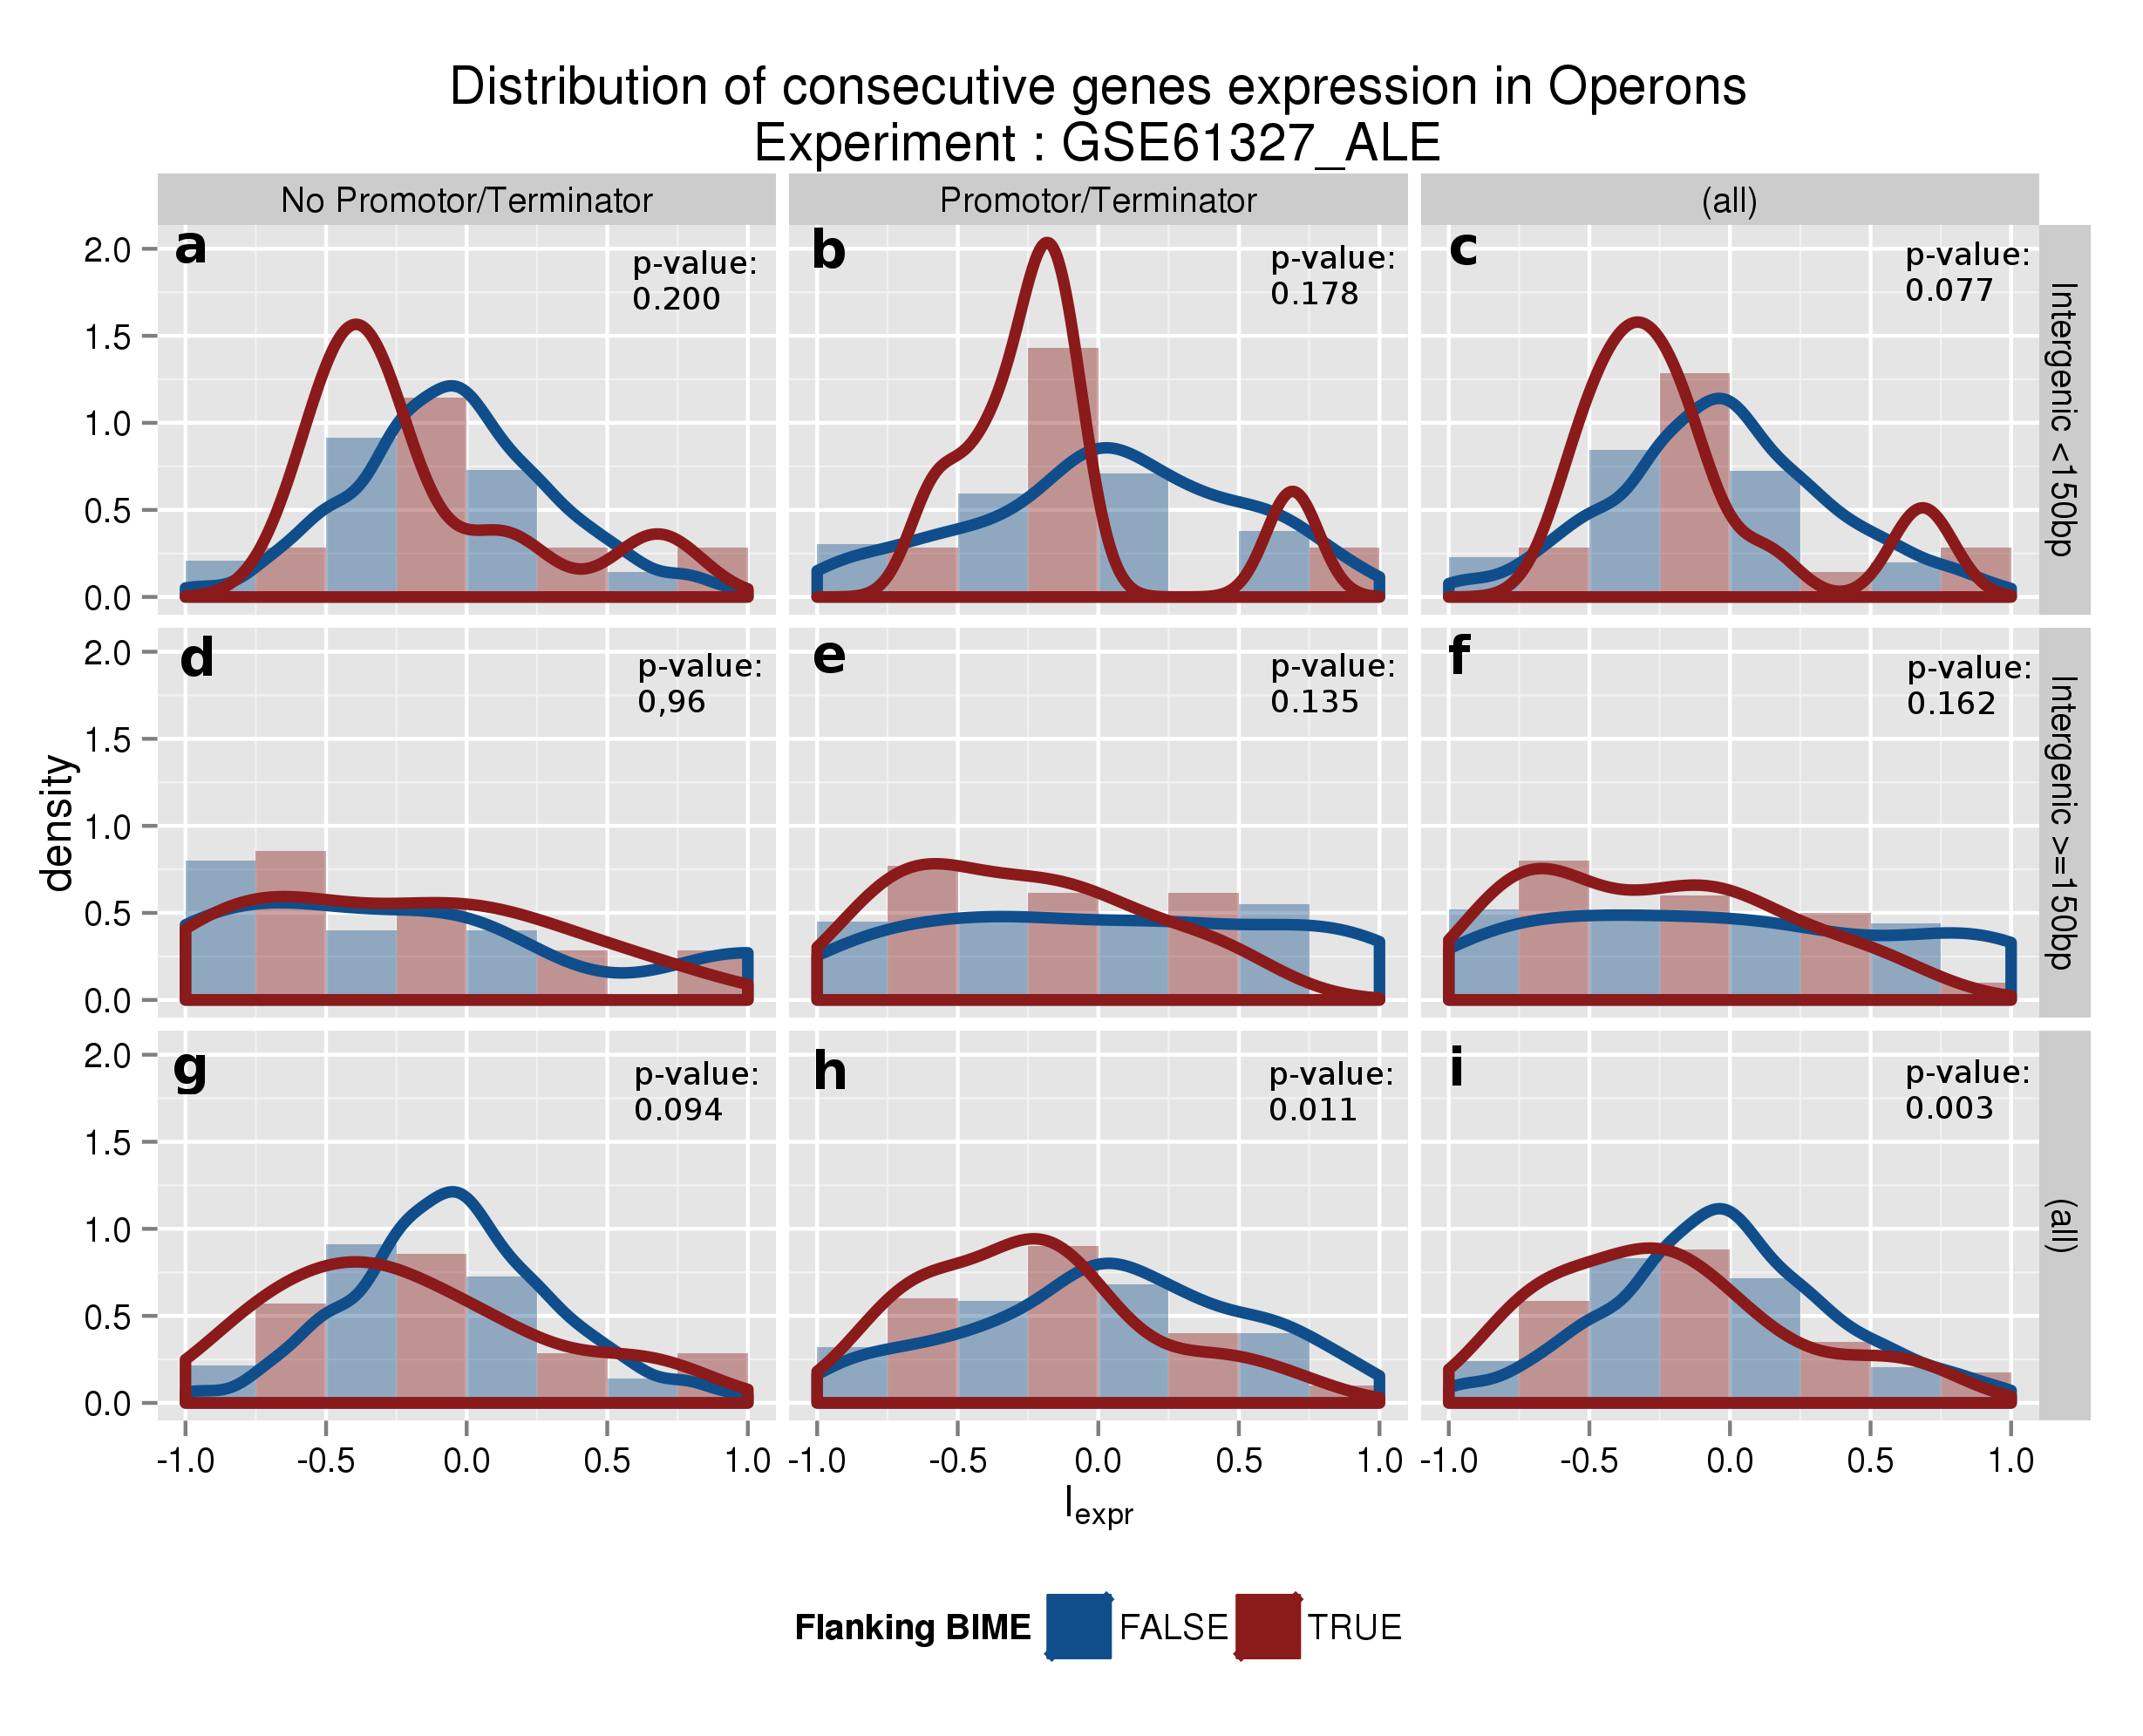
\includegraphics[scale=0.2]{figures/genesOperon_histoDens_GSE61327_ALE.png}}
\caption{\textbf{Niveau d'expression des gènes consécutifs dans les opérons.} Les données proviennent de l'expérience GSE61327\_ALE. L'$I_{expr}$ en abscisses est l'indice d'expression du gène 1 par rapport au gène 2 $(gene2 - gene1) / (gene2 + gene1)$, borné sur [-1,1]. Les valeurs négatives indiquent un niveau d'expression plus élevé du gène 1, les valeurs positives l'inverse. Les éléments de couleur rouge se réfèrent aux gènes flanquant une BIME, ceux en bleu aux gènes sans BIME entre eux. Les histogrammes indiquent la densité pour chacune des valeurs de l'$I_{expr}$. Les courbes de densité montrent la tendance de l'$I_{expr}$ par rapport à la présence/absence de BIME, la comparaison entre les 2 distributions est réalisée à l'aide d'un test de rang de Wilcoxon dont la p-valeur est affichée dans chaque graphique. Les graphiques sont décomposées sur 2 critères, les ET dans la RIG et la taille de la RIG (<150 pb ou >= 150 pb).}
\label{fig:expression_operon}
\end{figure}

L'analyse menée sur ce jeux de données est représentative des deux autres jeux de données malgré quelques différences (Voir annexe \ref{annexeOperon}). En raison des faibles effectifs de certains jeux de données et de l’écart à la distribution normale de plusieurs distributions, nous avons utilisé le test de rang de Wilcoxon (p-valeur < 0.05) pour tester l’égalité des médianes entre paires de gènes contenant une BIME dans la RIG et paires de gènes sans BIME dans la RIG (\autoref{fig:expression_operon}).
En absence de BIME nous observons une répartition symétrique du niveau d'expression des deux gènes centrée sur une valeur d'$I_{expr}$ à zéro (\autoref{fig:expression_operon} - (b,e,h)).
En prenant en compte la présence/absence de BIME et en s'intéressant dans un premier temps aux RIG de moins de 150 pb, en présence de promoteur/terminateur, le test statistique ne montre pas de différence entre l'écart des médianes des deux distributions (\autoref{fig:expression_operon} - (a,b,c)), mais nous distinguons clairement une distribution bi-modale avec les BIME qui n'est pas présente en leur absence et nettement plus marquée en présence d'ET (\autoref{fig:expression_operon} - (b)). Ceci est dû à la conjonction de l'effet des promoteurs d'un côté et des terminateurs amplifié par la présence des BIME de l'autre.
Pour les RIG de plus de 150 pb, nous observons un étalement des distributions avec un tendance légère allant vers un niveau d'expression plus important du gène 1 (\autoref{fig:expression_operon} - (d,e,f)).
En étudiant maintenant le facteur promoteur/terminateur sans se soucier de la taille de la RIG, nous remarquons toujours une tendance à l'expression plus importante du gène 1 qui devient significative en présence des ET ainsi qu'avec toutes les données (\autoref{fig:expression_operon} - (h,i)). 

Avec les trois jeux de données, nous observons un aplatissement de la courbe des paires de gènes qui ne contiennent pas de BIME dans leur RIG. Ce phénomène peut être dû au fait que nous n’avons pas distingué les promoteurs des terminateurs de transcription, signaux qui ont des effets antagonistes sur la transcription des gènes. Pour tester cette hypothèse, nous avons repris les mêmes données sans faire la distinction sur la taille de la RIG mais en décomposant les résultats suivant la présence de promoteurs, de terminateurs ou des deux annotés dans la RIG. Les résultats reportés \autoref{fig:expression_operon_reg}-(a) montrent un effet des promoteurs avec une expression plus importante du gène 2 (courbe verte) et l'effet inverse pour la courbe des terminateurs de transcription (courbe orange). Ces deux effets sont visibles de façon similaire sur la courbe des promoteurs et terminateurs (courbe violette). Quant à la courbe des RIG sans ET, elle est symétrique et centrée sur sur une valeur négative mais proche de zéro (-0.049). Un contrôle statistique par un test de Wilcoxon a été réalisé entre les valeurs d'$I_{expr}$ sans ET (courbes bleues) dans la RIG et chacun des trois autres cas de figure pour les trois jeux de données (\autoref{table:p-val_reg}). 

\begin{SCfigure}[][h!]
\fbox{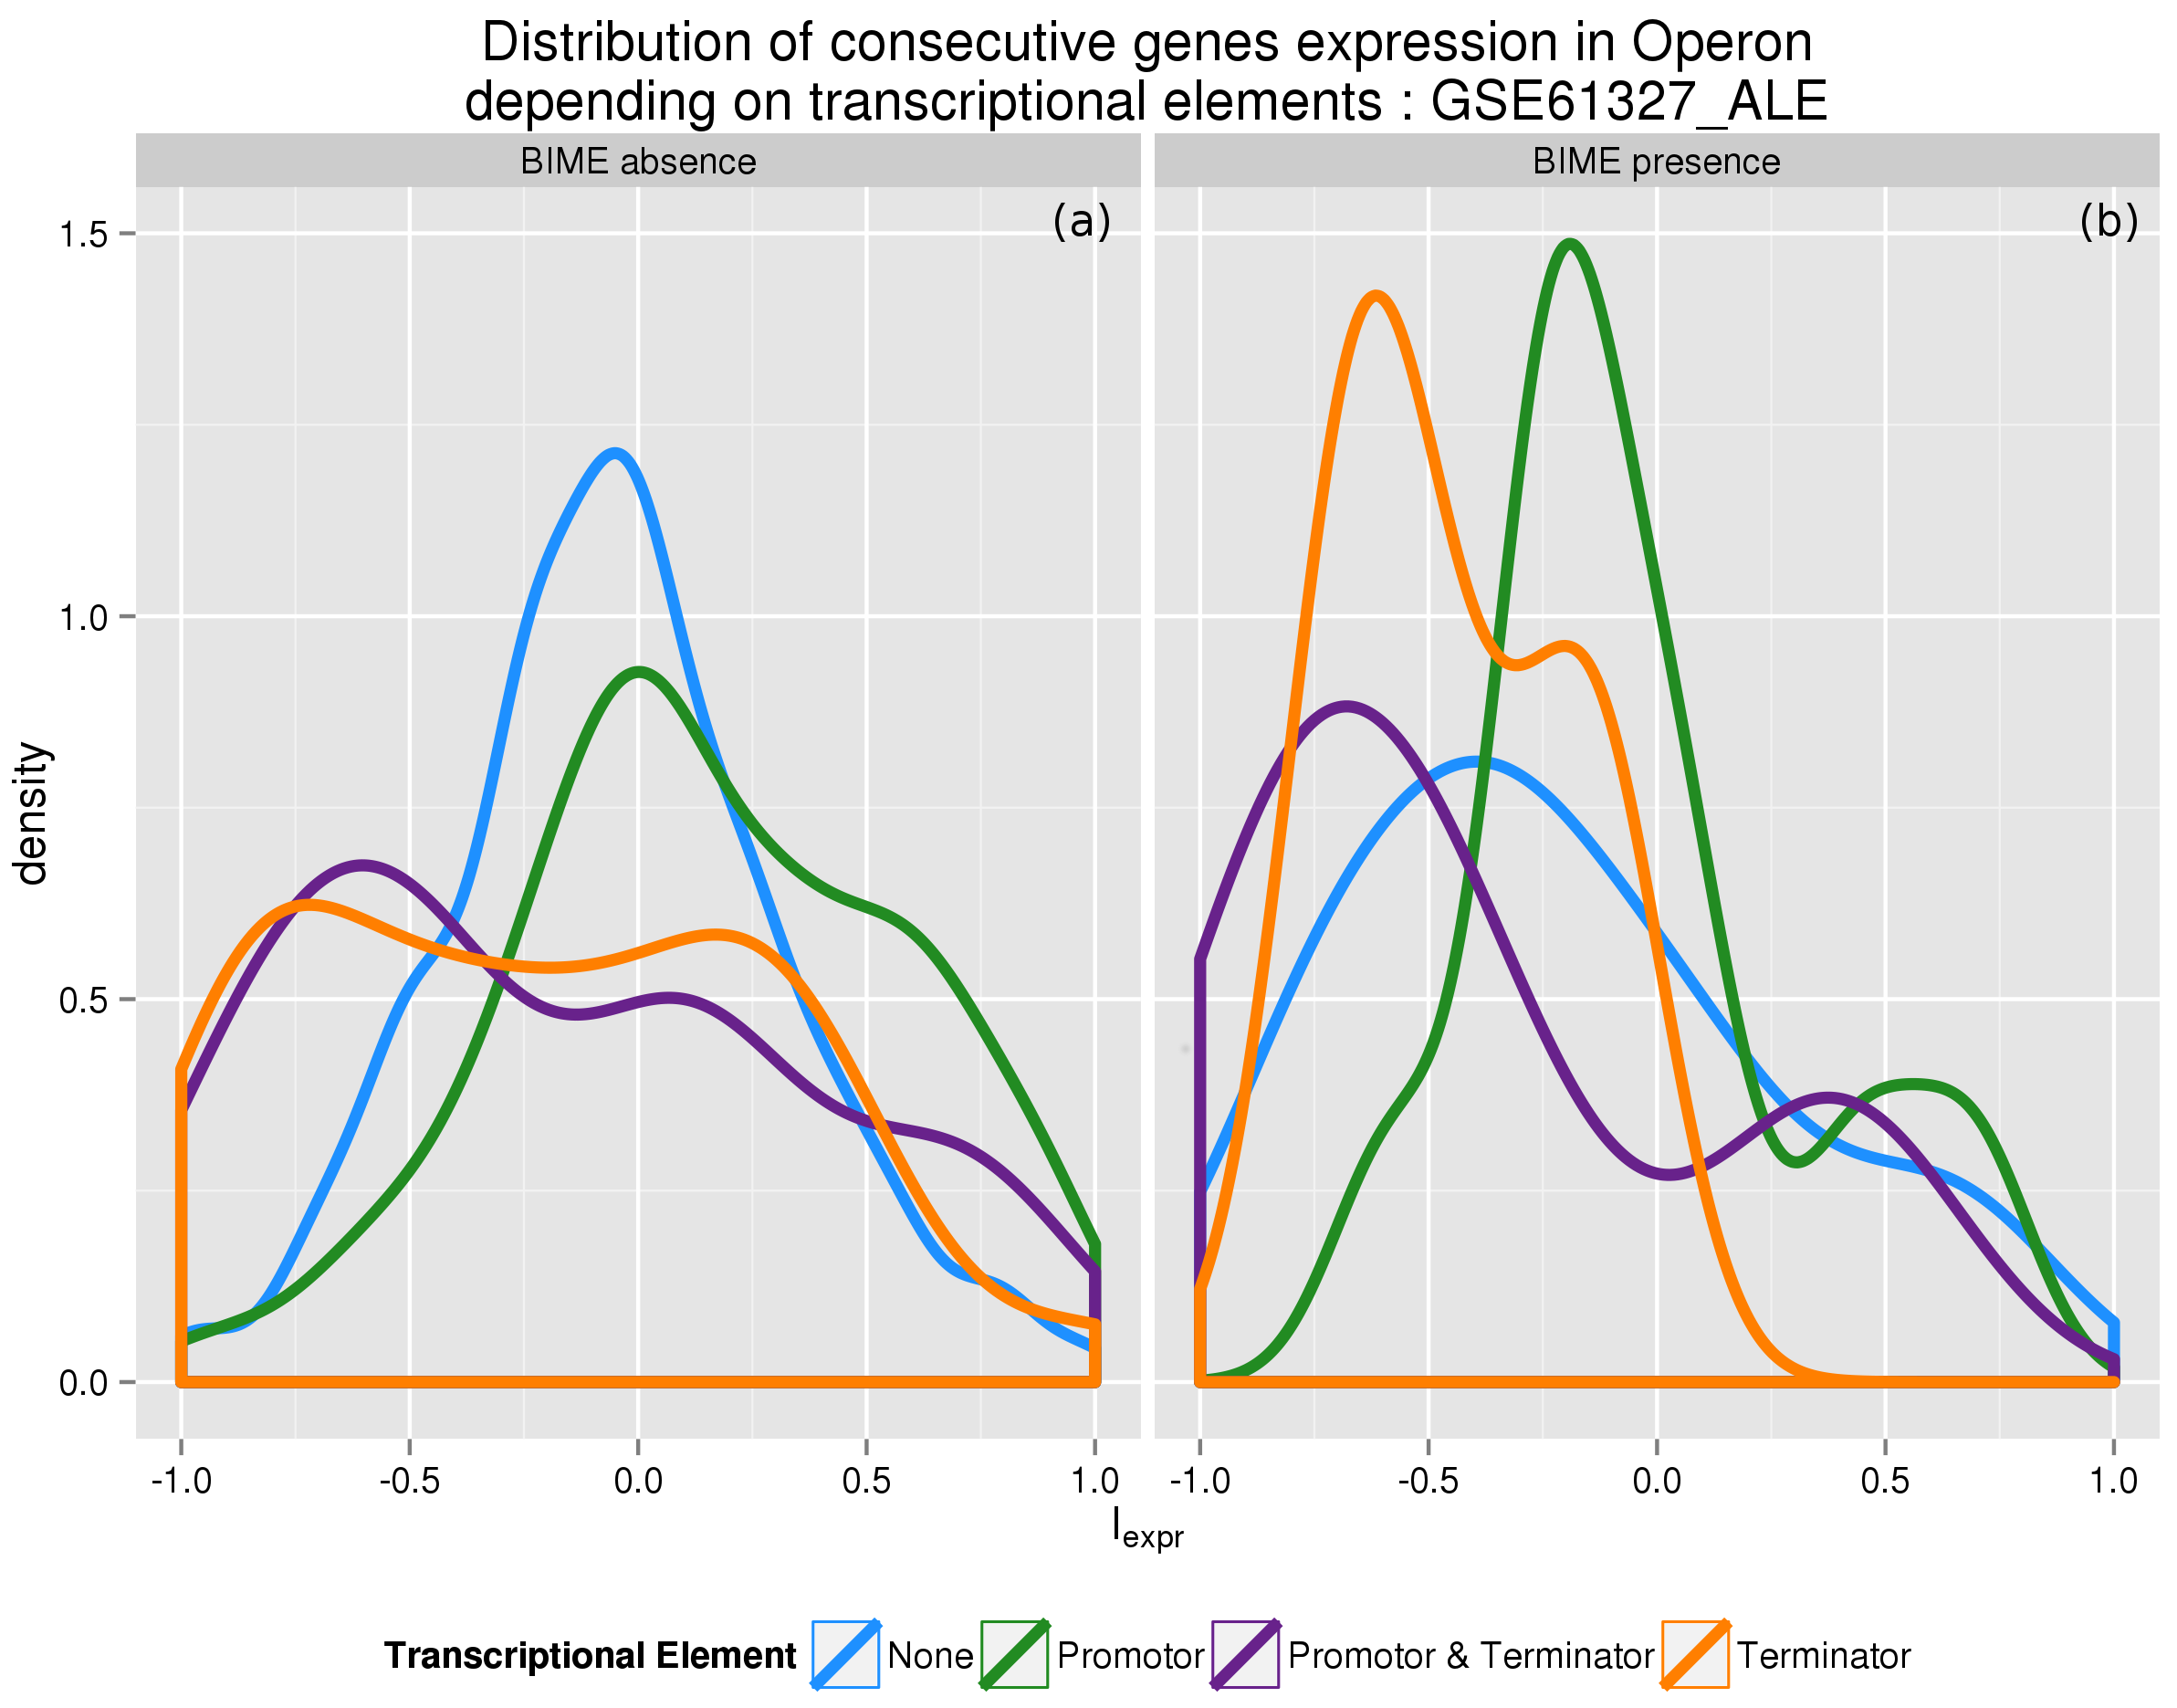
\includegraphics[scale=0.12]{figures/genesOperonReg_histoDens_GSE61327_ALE.png}
\caption{\textbf{Niveau d'expression des gènes consécutifs dans les opérons en fonction des éléments transcriptionnels (ET).} L'$I_{expr}$ en abscisses est l'indice d'expression du gène 1 par rapport au gène 2 $(gene2 - gene1) / (gene2 + gene1)$, borné sur [-1,1]. Les valeurs négatives indiquent un niveau d'expression plus élevé du gène 1, les valeurs positives l'inverse. Les courbes de densité indiquent la distribution de l'$I_{expr}$ en fonction des ET présent dans la RIG. Les courbes bleues indiquent l'absence de promoteur et/ou de terminateur de transcription, les vertes la présence de promoteur uniquement, les oranges la présence de terminateurs de transcription uniquement et les violettes la présence à la fois de promoteurs et de terminateurs transcription. \textbf{(a)} présence de BIME dans la RIG, \textbf{(b)} absence de BIME dans la RIG.
\label{fig:expression_operon_reg}}}
\end{SCfigure}

En absence de BIME, les résultats nous indiquent qu'il existe une différence significative entre les médianes des distributions sans ET et les trois autres (p-valeurs < 0.05), résultat attendu puisque les ET ont un effet sur la transcription des gènes. En revanche dans le cas où les BIME sont présentes (\autoref{fig:expression_operon_reg}-(b)), uniquement la distribution de l'$I_{expr}$ contenant des promoteurs se différencie de manière significative de celle sans ET (sauf pour GSE61327\_ALE), visible également sur le graphique avec un décalage de toutes les courbes vers une expression plus importante du premier gène. 
En s'intéressant à la position des terminateurs de transcription par rapport à celles des 39 BIME des opérons, nous avons observé que 14 BIME chevauchent des terminateurs. Ce résultat nous conforte dans l'hypothèse que les BIME joueraient un rôle similaire aux terminateurs de transcription ou de stabilisation de la partie 5' du transcrit face au dégradosome.

\begin{table}[h!]
\centerline{
\begin{tabular}{|c|c|c|c|c|}
  \hline
  \rowcolor{Gray} Tests & Données & Promoteur & Terminateur & Promoteur \& Terminateur\\
  \hline
  \multirow{3}{*}{Absence de BIME}& GSE61327\_ALE & $5.47~e^{-11}$ & $7.65~e^{-3}$ & $0.033$ \\ 
  \cline{2-5}
  & HS-15min & $5.48~e^{-14}$ & $7.30~e^{-5}$ & $0.009$ \\
  \cline{2-5}
  & M-P4h & $5.78~e^{-12}$ & $1.43~e^{-7}$ & $0.017$ \\
 \hline
 \multirow{3}{*}{Présence de BIME}& GSE61327\_ALE & $0.259$ & $0.444$ & $0.441$ \\ 
  \cline{2-5}
  & HS-15min & $0.034$ & $0.375$ & $0.921$ \\
  \cline{2-5}
  & M-P4h & $0.035$ & $0.274$ & $0.767$ \\
  \hline
\end{tabular}}
\caption{\textbf{P-valeurs des tests de rang de Wilcoxon des $I_{expr}$ en présence/absence de BIME dans les cas de RIG sans ET par rapport aux différents ET présents dans les RIG sur les 3 jeux de données.}
\label{table:p-val_reg}}
\end{table}

Afin d'approfondir ces hypothèses, nous avons étudié plus en détail le niveau d'expression des gènes dans les 36 opérons contenant des BIME.

\section*{Impact des BIME au niveau des paires de gènes}
\label{expression_operon}

Dans l’expérience précédente nous avons observé des tendances globales sur les biais du taux d’expression en présence de BIME. Nous allons maintenant identifier les paires de gènes qui présentent des différences de taux d’expression significatives. Pour cela, nous avons calculé, pour chaque gène, les moyennes des RPKM obtenus avec les différents réplicats et nous avons comparé les moyennes des gènes localisés de part et d’autre d’une RIG contenant une BIME. Encore une fois le faible effectif des échantillons nous a conduits à utiliser le test de Wilcoxon pour tester l’égalité des médianes. Nous avons retenu comme paires de gènes différentiellement exprimés celles dont le test de Wilcoxon donne une p-valeur < 0,01. Dans ce cadre, les opérons contenant des BIME sont sélectionnés et l'expression des deux gènes de l'opéron flanquant la BIME prise en compte si au moins un des deux gènes a une couverture > 10, cette valeur est choisie car elle représente le premier quartile de nos données, supprimant les gènes les moins exprimés.

Afin de facilité l’interprétation des résultats, nous avons écrits deux fonctions pour générer des représentations graphiques. La première est une visualisation graphique du test réalisé représentant les niveaux d’expression normalisés des gènes de l'opéron ainsi que la position relative des REP formant la BIME (Figure \autoref{fig:expressionFigA}). La seconde est une représentation de la couverture des reads au niveau de la région chromosomique codant pour l’opéron par rapport à l'organisation génomique de celui-ci ainsi que la catégorisation des REP composant la BIME (Figure \autoref{fig:expressionFigB}). Elle permet d’analyser plus finement la contribution de la BIME dans les variations de la couverture.

\begin{figure}[h]
\centering
\subfigure[]{\label{fig:expressionFigA} 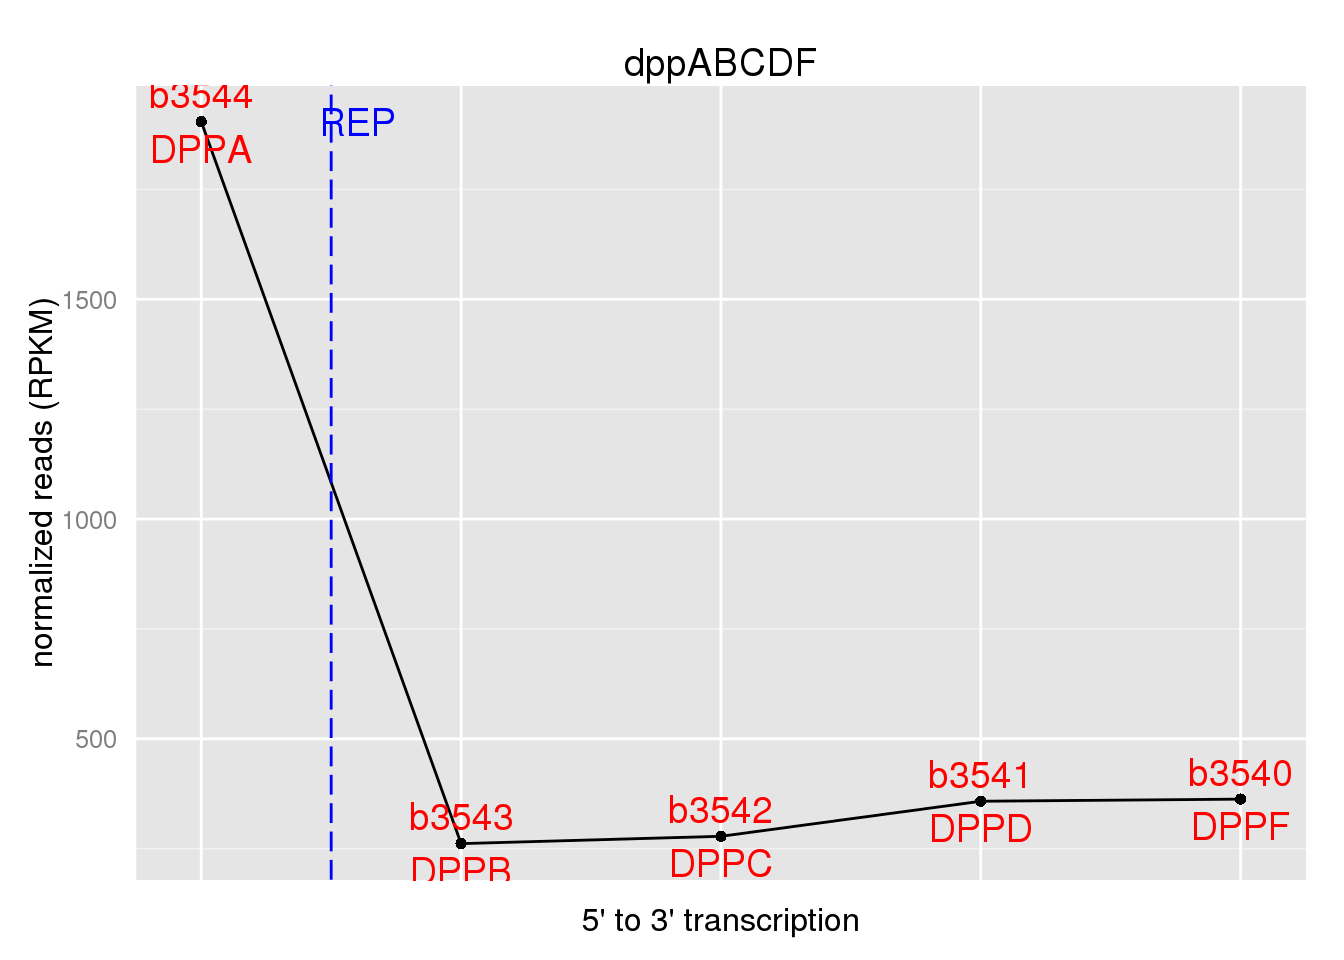
\includegraphics[scale=0.35]{figures/expression1.png}}
\subfigure[]{\label{fig:expressionFigB} 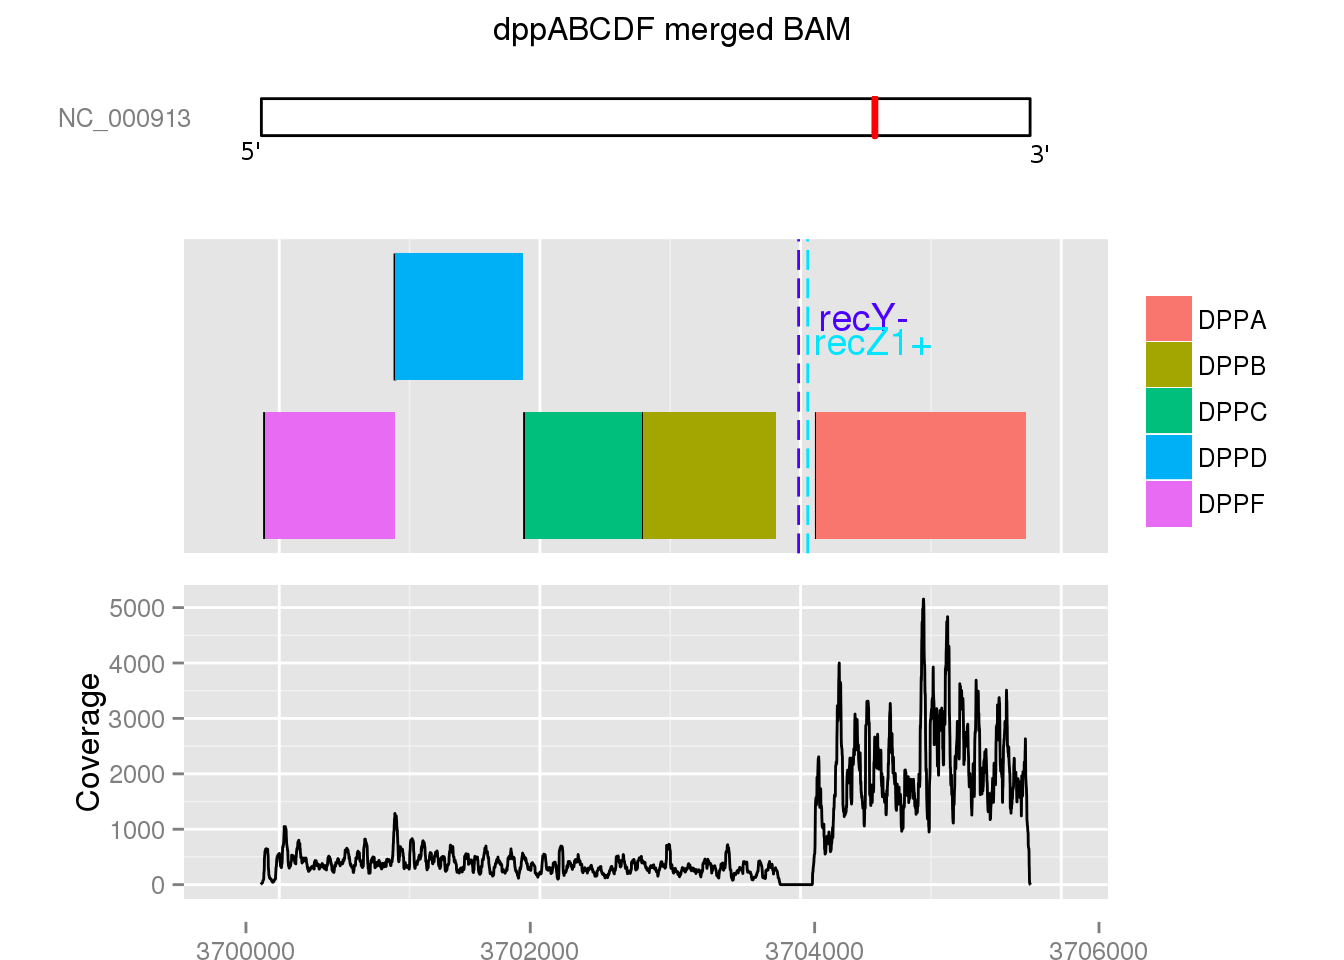
\includegraphics[scale=0.35]{figures/expression2.png}}
\caption{\textbf{Résultats de l'étude de l'expression des gènes dans les opérons contenant des BIME. (a)} Le niveau d'expression normalisé de chaque gène de l'opéron est représenté en ordonnées, l'organisation des gènes de l'opéron est schématisée sur l'axe des abscisses dans le sens 5' $\mapsto$ 3', l'orientation du brin est notée sur l'axe des abscisses. Les barres noires verticales représentent l'erreur standard à la moyenne. La position de la ou les REP composant la BIME est schématisée par la ligne bleue verticale. En tenant compte de l'orientation du brin, si au moins un promoteur ou un terminateur de transcription est présent dans la RIG contenant la BIME, ceux-ci sont représentés respectivement par une ligne en pointillés verticale verte ou rouge. \textbf{(b)} La position de l'opéron sur le génome est indiquée par la barre rouge sur l'idéogramme de la partie supérieure. La partie médiane représente l'organisation des gènes de l'opéron dans le sens 5' $\mapsto$ 3' (l'orientation du brin est précisée dans le titre) ainsi que le positionnement et la classe des REP composant la BIME. La partie inférieure montre la couverture issue des fichiers BAM fusionnés de l'expérience par rapport à l'organisation de la partie médiane.}
\label{fig:expression} 
\end{figure}

Nous avons testé cette méthode sur les trois jeux de données qui ont produit les résultats du \autoref{table:expression}.

\begin{table}[h!]
\centerline{
\begin{tabular}{|l|c|c|c|c|}
  \hline
  \rowcolor{Gray} Jeux de données & $\frac{Nb.~operons~avec~genes~DE}{Nb.~d'operons~exprimes}$ \scriptsize{\dag} & \begin{tabular}{c}Nb. de RIG\\avec Terminateurs\end{tabular}\\ 
  \hline
  GSE61327\_ALE & 17/32 & 7/17\\  
  \hline
  HS-15min & 8/20& 1/8\\ 
  \hline
  M-P4h & 12/30& 4/12\\
 \hline
\end{tabular}}
\caption{\textbf{Résultats de l'étude de différence d'expression des gènes des opérons flanquant une BIME.} \scriptsize{\dag} Nombre d'opérons contenant 2 gènes flanquant une BIME pour lesquels nous observons une différence de niveau d'expression sur le nombre d'opérons dont les 2 gènes flanquant la BIME sont exprimés (au moins un des 2 gènes possède une couverture > 10).
\label{table:expression}}
\end{table}

Sur les résultats obtenus, nous constatons tout d'abord une hétérogénéité du nombre d'opérons exprimés. Concernant les terminateurs de transcription présent dans la RIG contenant la BIME, 2/7 se situent avant la BIME, 3/7 la chevauchent et 2/7 sont après pour GSE61327\_ALE. Le terminateur est situé après la BIME pour HS-15min. Pour M-P4h, un seul terminateur est situé avant la BIME, 2/4 la chevauchent et un seul est situé après. \textcolor{red}{Le phénomène de colocalisation des BIME et des terminateurs pourrait indiquer un rôle de la BIME dans la terminaison de transcription ou tout du moins d'atténuation dans les opérons car dans les six cas de chevauchement avec le terminateur, nous observons un niveau d'expression diminué du second gène par rapport au premier.}

\begin{SCfigure}[][h!]
\fbox{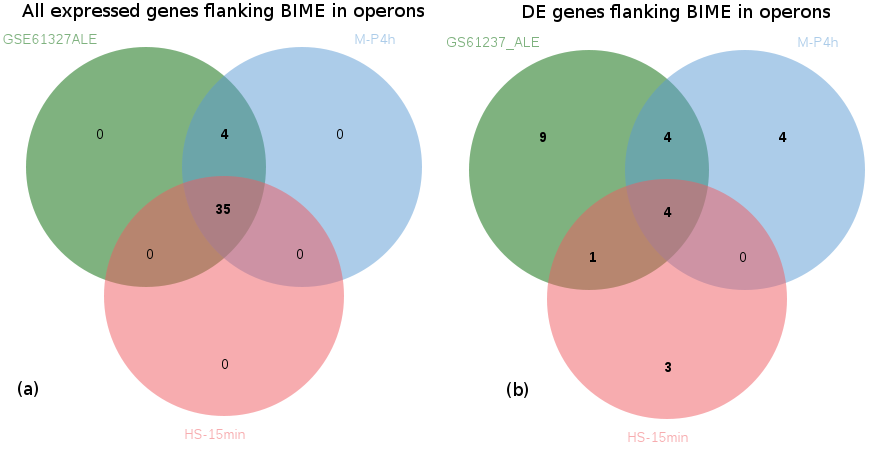
\includegraphics[scale=0.33]{figures/jVenn_expr.png}
\caption{\textbf{Diagrammes de Venn des paires de gènes exprimés et flanquant une BIME dans un opéron pour les 3 jeux de données.} Représentation réalisée sur le logiciel \texttt{jVenn} \citep{Bardou2014}, en vert est représenté le jeux de données GSE61327\_ALE, en rouge HS-15min et en bleu M-P4h. \textbf{(a)} Toutes les paires de gènes flanquant un BIME dont le niveau d'expression d'au moins un des 2 gènes est supérieur à 10. \textbf{(b)} Toutes les paires de gènes flanquant un BIME dont le niveau d'expression d'au moins un des 2 gènes est supérieur à 10 et pour lesquels une DE a été détectée statistiquement (p-valeur < 0.01). 
\label{fig:jVenn_expr}}}
\end{SCfigure}

Nous avons également comparé les paires de gènes flanquant un BIME qui sont exprimés dans les trois jeux de données. 37 paires de gènes sont exprimées dans les trois jeux de données et 4 dans deux (un opéron pouvant contenir plusieurs BIME), ce qui nous indique une expression de tous ces opérons indépendamment du jeux de données (\autoref{fig:jVenn_expr}-a). En revanche, si nous nous intéressons aux paires de gènes DE nous observons beaucoup plus de variations (\autoref{fig:jVenn_expr}-b), ce phénomène est une surprise car nous nous attendions à voir des recouvrements similaires. Il sera discuté par la suite.

\section*{Localisation des variations de taux d'expression}

Des résultats précédents, il découle que les variations du taux d’expression entre paires de gènes peuvent être dues à la présence de différents type de structure au niveau de l’ARNm comme les BIME mais aussi les signaux de transcription. Afin de mieux appréhender la contribution des BIME, nous avons mis en œuvre deux méthodes exploitant les profils d’expression : une approche locale basée sur une fenêtre glissante (cf. page~\pageref{methode_correlation}) et une approche plus globale reposant sur la segmentation (cf. page~\pageref{methode_segmentation}). 

\subsection*{Approche locale}
\label{approche_locale}
Nous avons développé une méthode réalisant un test de corrélation entre les profils d'expression des régions contenant des BIME et un profil modèle de changement d'expression en modifiant la technique décrite page~\pageref{methode_correlation}. Elle a été adaptée pour nous permettre de localiser le point de cassure dans la RIG contenant une BIME. Nous avons privilégié une approche locale en effectuant la recherche de points de cassure dans une fenêtre dont nous avons fixé la taille et qui parcourt des régions d'intérêt pour 2 gènes consécutifs au sein d'un opéron dont le niveau d'expression se différencie. Ces régions d'intérêt commencent à la 1\up{ère} position du gène 1 et finissent à la dernière position du gène 2. Une fois ces régions extraites, le calcul de la couverture base par base a été réalisé à l'aide des BEDtools (Annexe \ref{annexeCode}).

Nous avons adapté certains paramètres de la méthode originelle. Le choix de la taille de la fenêtre glissante a été motivé par plusieurs raisons, suite à des essais nous sommes arrivés aux conclusions qu'une fenêtre trop petite (100 pb) présente une sensibilité trop importante aux variations locales dues au manque d'uniformité de la couverture (cf. page~\pageref{uniformite_couverture}), alors qu'une fenêtre de taille trop grande (500 pb) produit une perte de sensibilité en lissant les couvertures de chaque moitié de la fenêtre. La taille des BIME a été augmentée de 40 pb de chaque côté (taille moyenne d'une REP) afin d'identifier les points de cassure se situant aux limites de la BIME. Après avoir réalisé une série d'essais, la valeur du seuil de corrélation a été ajustée de 0.7 à 0.5 afin de détecter un nombre de points de cassure suffisamment important, avec une corrélation encore considérée comme forte dans la littérature, sans pour autant obtenir trop de faux positifs du fait du faible seuil de la p-valeur du test de corrélation. Finalement nous avons introduit un filtre supplémentaire quant à la couverture minimale d'un des deux gènes devant être au moins supérieure à 10. Les critères de la méthode sont :

\begin{itemize}[label=$\bullet$]
\item fenêtre glissante de 300 bases
\item au moins un des deux gènes possède une couverture > 10
\item $log_2(\frac{\overline{couverture~droite}~+~1}{\overline{couverture~gauche}~+~1})~\geq~1$ pour un profil \_\_\_|\^{ }\^{ }\^{ }
\item $log_2(\frac{\overline{couverture~gauche}~+~1}{\overline{couverture~droite}~+~1})~\geq~1$ pour un profil \^{ }\^{ }\^{ }|\_\_\_
\item une corrélation > 0.5 avec une p-valeur $< 10^{-7}$
\end{itemize}

Pour chaque fenêtre, nous obtenons une corrélation associée à une p-valeur. Les points de transition d’expression sont identifiés comme des maximums locaux de la corrélation sur les régions ayant une suite consécutive de p-valeur $< 10^{-7}$.

Deux types de fichiers sont générés au format \texttt{bedgraph} pour une visualisation sur un Genome Browser, le premier sous forme de diagramme de barre représentant les couvertures moyennes des deux parties de la fenêtre, le second représentant l'évolution de la corrélation sur la zone (\autoref{fig:igv_profil}). Une représentation des niveaux d'expression moyens des 2 gènes et de la BIME est également générée sous forme de diagramme de barres avec les informations de sens et du type de la BIME (\autoref{fig:profil_plot}). Sur les deux représentations graphiques, nous pouvons à nouveau observer le biais du taux d'expression des BIME avec une déplétion de la couverture de l'ordre de ce que nous avions observé \autoref{fig:same_expression_operon_point}, phénomène visible sur de nombreux résultats de cette méthode. Les résultats de cette approche sont présentés dans le \autoref{table:profil}.

\begin{figure}[h!]
\centerline{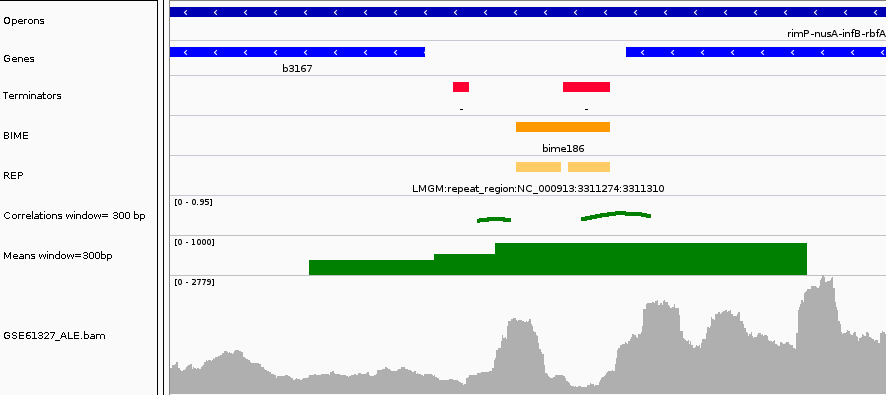
\includegraphics[scale=0.53]{figures/igv_profil.png}}
\caption{\textbf{Visualisation des changements de couverture obtenus par la méthode de corrélation des profils.} L'opéron est de couleur violette, les gènes sont en bleu, les promoteurs en vert clair, les terminateurs de transcription en rouge, les BIME sont représentées en orange foncé, les REP en orange clair. La courbe verte indique l'évolution de la corrélation dans la région délimitée par les valeurs significatives du test de corrélation. Le diagramme de barres en vert aux dimensions de la fenêtre montre les profils d'expression moyens de chacune de ses moitiés et est centré sur le maximum de la courbe de corrélation. Le brin sur lequel sont les éléments est indiqué par le sens des chevrons sur les opérons, gènes, promoteurs et par un signe sous les terminateurs. Dans cet exemple, le changement d'expression indique une diminution du niveau d'expression sur le brin complémentaire avec la valeur de corrélation la plus importante située sur la BIME.} 
\label{fig:igv_profil}
\end{figure}

\begin{SCfigure}[][h!]
\fbox{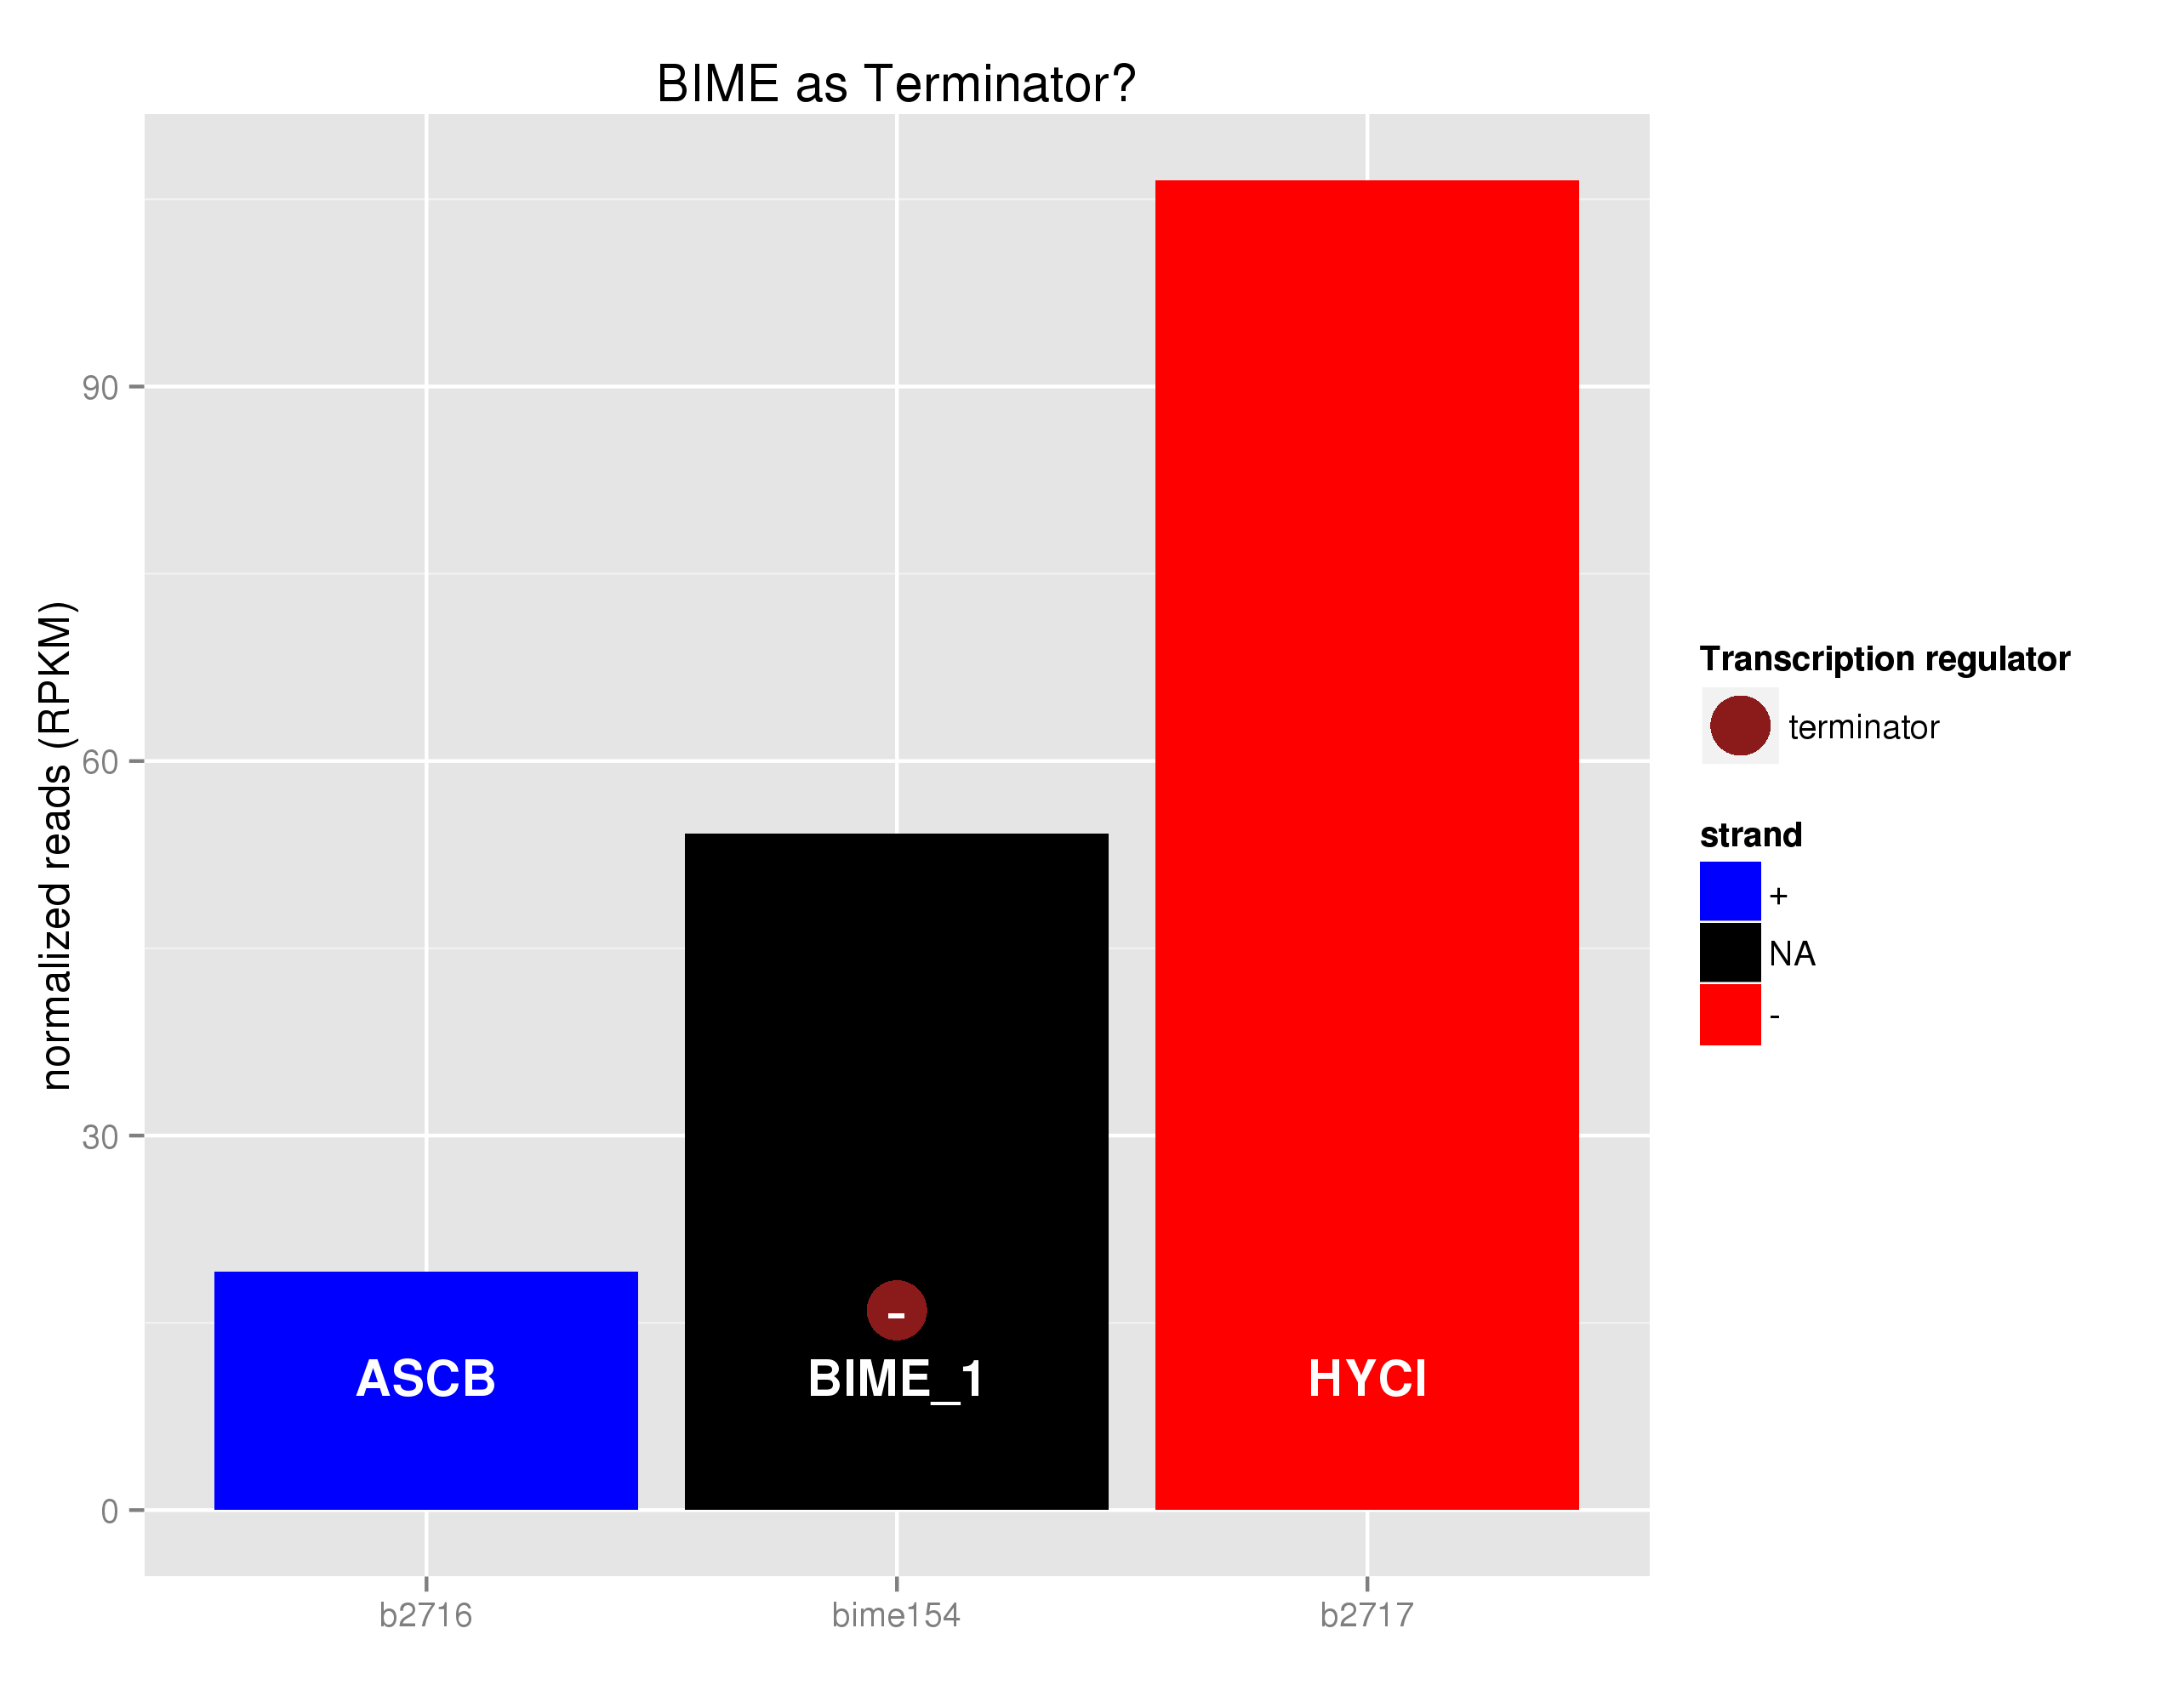
\includegraphics[scale=0.5]{figures/profil_plot.png}
\caption{\textbf{Résultat de corrélation de profils.} Les niveaux d'expression moyens des gènes encadrant la BIME et de cette dernière sont représentés par diagrammes de barre (même cas que pour la \autoref{fig:igv_profil}). La couleur du diagramme indique le sens de transcription de l'élément, bleu pour le brin direct, rouge pour le brin complémentaire et noir lorsque aucun brin est défini. La présence d'éléments de régulation dans la RIG est représentée par des ronds de couleur verte pour les promoteurs et rouge pour les terminateurs de transcription avec un symbole '+' ou '-' pour indiquer le sens du brin de cet élément. La représentation est schématique et ne donne pas d'information sur la position exacte de ces éléments ni sur leur nombre.}
\label{fig:profil_plot} }
\end{SCfigure}

\begin{table}[h!]
\centerline{
\begin{tabular}{|l|c|c|}
  \hline
  \rowcolor{Gray} Jeux de données &\begin{tabular}{c} Nb. de points\\de cassure détectés \end{tabular} & \begin{tabular}{c}Présence de\\promoteurs et/ou terminateurs\end{tabular}\\ 
  \hline
  GSE61327\_ALE & 12 & 5/12  \\  
  \hline
  HS-15min & 5 & 0/5 \\ 
  \hline
  M-P4h & 5 & 2/5  \\
 \hline
\end{tabular}}
\caption{\textbf{Résultats de l'étude par la méthode de corrélation sur les gènes des opérons flanquant une BIME.}
\label{table:profil}}
\end{table}

Pour les données GSE61327\_ALE, 12 points de cassures sont détectés sur les 32 opérons contenant des gènes DE flanquant une BIME et 5 d'entre eux pourraient être sous l'effet d'un promoteur ou terminateur de transcription et donc difficilement interprétables. Sur les 7 cas restant, 6 montrent un niveau d'expression plus important du 1\up{er} gène. Le 7\up{ème} cas, niveau d'expression plus élevé du 2\up{ème} gène est difficilement explicable, peut-être la présence d'un promoteur non annoté. Pour les 2 autres jeux de données, 5 points de cassure sont détectés et seul l'expérience M-P4h montre 2 points de cassure possiblement causés par la présence d'un promoteur ou un terminateur. Les autres points de cassure ne peuvent être lié qu'à la présence des BIME et pour tous lorsque le niveau d'expression du 1\up{er} gène est plus important.
Ces résultats vont également dans le sens de ce que nous avions découvert en s'intéressant aux niveaux d'expression des gènes des consécutifs en présence de BIME des opérons dans la partie précédente avec un rôle possible de terminateur ou du moins atténuateur de transcription des BIME ou également un rôle de stabilisation de la partie 5' du transcrit face au dégradosome.

Une des faiblesses de cette approche est sa sensibilité aux variations locales des couvertures de reads, en particulier pour les jeux de données avec un faible nombre de réplicats mais également à la sous-représentation systématique des reads au niveau des BIME. Cela conduit à une plus faible sensibilité de la méthode et à une forte propension à prédire des variations multiples d’expression dans la même RIG.

\subsection*{Approche par segmentation}
Nous avons voulu tester si les faiblesses observées avec la méthode locale peuvent être compensées par une méthode de segmentation n'utilisant pas de comparaison de profils et prenant en compte la globalité de la région étudiée telle que décrite dans la section précédente.
En reprenant la méthode décrite page~\pageref{methode_segmentation}, nous avons fixé le paramètre $K$ à 4 segments maximum donc 3 points de cassure de façon à vérifier la présence éventuelle de plusieurs de ces points sur la RIG. Ce critère de 4 segment nous permettra de détecter des points cassures pouvant être dus à la fois à la présence de promoteurs, de terminateurs de transcription et de BIME. 
Dans notre étude, nous nous intéressons aux positions de ces points de cassures lorsqu'au moins un des deux gènes possède une couverture supérieure à 10. Les résultats sont croisés avec la présence de promoteurs ou de terminateurs de transcription dans la RIG et si les deux gènes appartiennent à un opéron, un test  statistique sur la différence d'expression est réalisé avec la même méthodologie que pour la partie~\nameref{expression_operon}. Seuls les paires de gènes dont le test est significatif sont étudiés.

\begin{SCfigure}[][h!]
\fbox{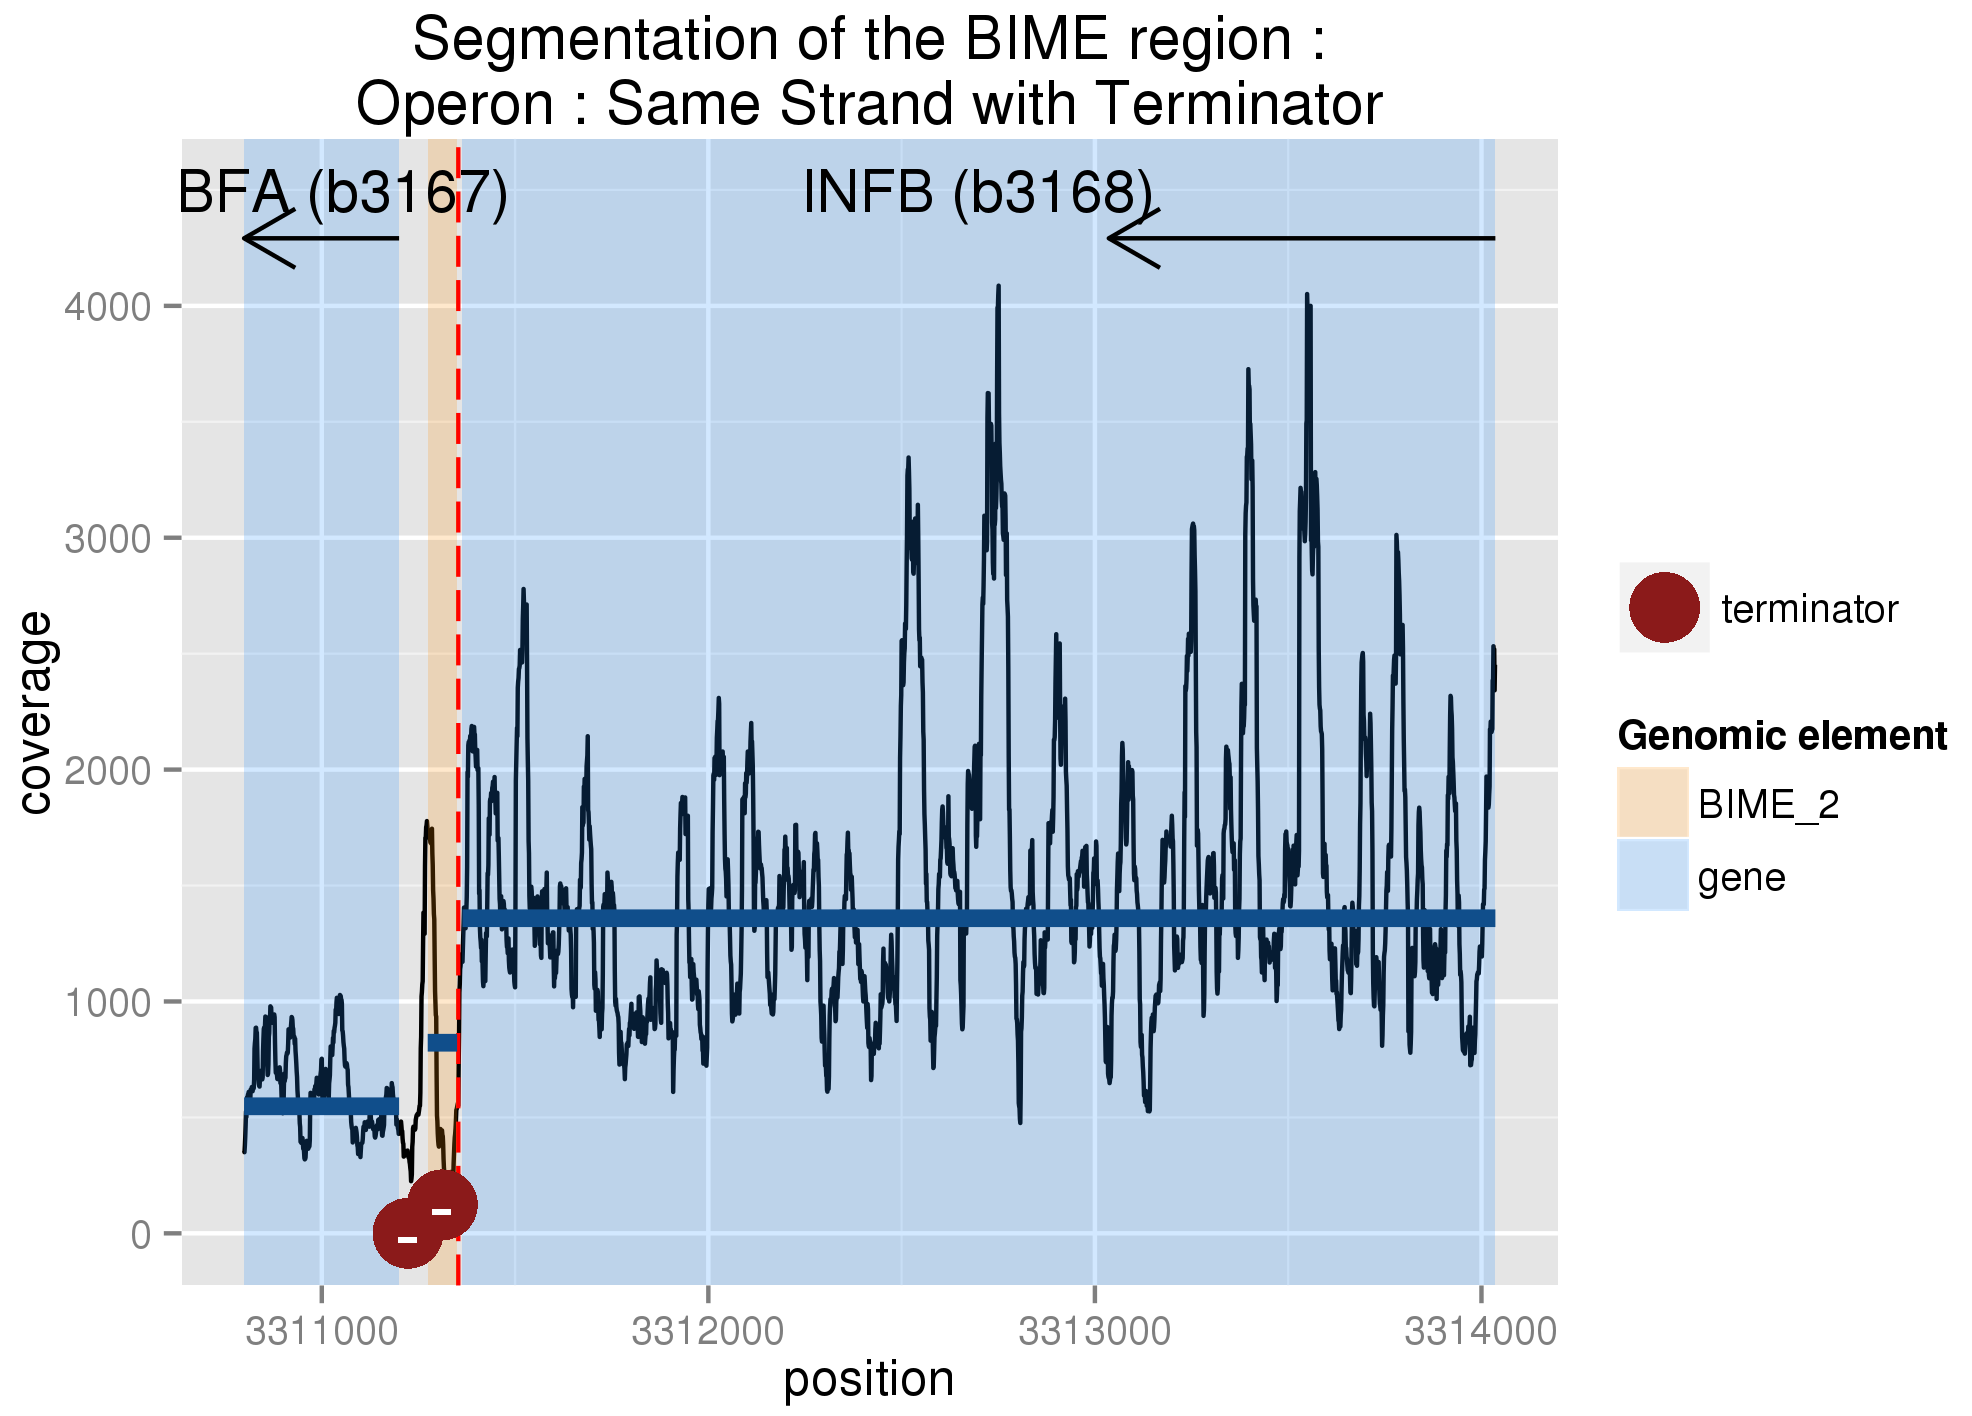
\includegraphics[scale=0.75]{figures/segmentation.png}
\caption{\textbf{Résultat de segmentation pour $K_{max} \mathord{=} 4$.} Les gènes sont symbolisés par les zones bleues, leur sens de transcription par les flèches noires. La BIME est représentée par la zone orange et sa classe est précisée dans la légende (Genomic element). Les promoteurs sont représentés par des points verts et les terminateurs par des points rouges, leurs orientations affichées par les symboles '+' ou '-' sur ces points. La courbe noire représente la couverture sur la région et les barres bleues horizontales indiquent les couvertures moyennes des éléments génomiques. Les points de cassure dans la couverture, déterminés par la segmentation, sont matérialisés par des lignes rouges verticales en pointillés.}
\label{fig:segmentation} }
\end{SCfigure}

Nous avons écrit un script R pour présenter les résultats sous forme graphique (\autoref{fig:segmentation}) et les résultats obtenus avec les différents jeux de données sont résumés dans le \autoref{table:segmentation}

\begin{table}[h!]
\centerline{
\begin{tabular}{|l|c|c|c|c|c|}
  \hline
  \rowcolor{Gray} Jeux de données &\begin{tabular}{c}Opérons avec\\point de\\cassure\\dans la RIG\\avec BIME\end{tabular} & \begin{tabular}{c}Présence\\d'ET\\dans la\\RIG\end{tabular} & \begin{tabular}{c}Points de\\cassure sur\\la BIME\end{tabular} & \begin{tabular}{c}Points de\\cassure\\sur BIME\\sans ET\end{tabular} & \begin{tabular}{c}BIME proche\\du gène le plus\\exprimé\\ sans ET\end{tabular}\\ 
  \hline
  GSE61327\_ALE & 15 & 7/15 & 12/15 & 8/12 & 11/12 \\  
  \hline
  HS-15min & 5 & 1/5 & 5/5 & 4/5 & 2/4\\ 
  \hline
  M-P4h & 2 & 0/2 & 2/2 & 2/2 & 1/2\\
 \hline
\end{tabular}}
\caption{\textbf{Résultats de l'étude par la méthode de segmentation sur les gènes des opérons flanquant une BIME.} 
\label{table:segmentation}}
\end{table}

Ces résultats sont proches de ceux obtenus sur le \autoref{table:expression} sauf pour le jeux de données M-P4h pour lequel très peu de changements de niveau d'expression sont détectés dans les opérons. La majorité des points de cassure sont détectés sur les BIME, ce qui va dans le sens d'une implication de ces dernières dans la régulation transcriptionnelle. Pour le jeu de données GSE61327\_ALE, la présence de promoteurs et de régulateurs est plus importante et seuls 3 cas sur 15 ont un point de cassure situé en dehors de la BIME (Données non montrées). Le nombre important de points de cassure situés sur la BIME pour les trois jeux de données, 12/15, 5/5 et 2/2, semblent indiquer un rôle des BIME dans la régulation de l'expression des gènes. Plus spécifiquement, si nous ne prenons que les cas sans promoteurs ou terminateurs, 8/15, 4/5 et 2/2, nous nous focalisons uniquement sur le rôle des BIME dans la régulation de l'expression des gènes de l'opéron et pouvons constater qu'elles semblent impliquées. Nous remarquons également que la BIME se trouve localisée à proximité du gène le plus exprimé dans un majorité de cas.

\section*{Évolution des structures des BIME}
Les analyses précédentes ont produits des résultats en détectant des différences de niveaux d'expressions ainsi que la localisation des points de cassures sur les BIME des gènes des opérons. Nous avons croisé ces résultats afin d'identifier les couples de gènes communs aux 3 méthodes. Nous observons 11 couples pour le jeux de données GSE61327\_ALE, 3 pour HS-15min et un seul pour M-P4h (Annexe \ref{annexeVenn}).
Les résultats obtenus suggèrent qu’au moins certaines BIME pourraient être impliquées dans la régulation de la transcription et/ou de la dégradation des ARNm. Si nous supposons que ce rôle dépend de leur capacité à se replier en une structure secondaire stable, alors ces BIME devraient subirent une pression de sélection positive afin de maintenir cette structure secondaire. Pour tester cette hypothèse, nous avons comparé la stabilité de la structure secondaire de la séquence ancêtre la plus ancienne avec celle présente chez E. coli contemporaines.

\begin{SCfigure}[][h!]
\fbox{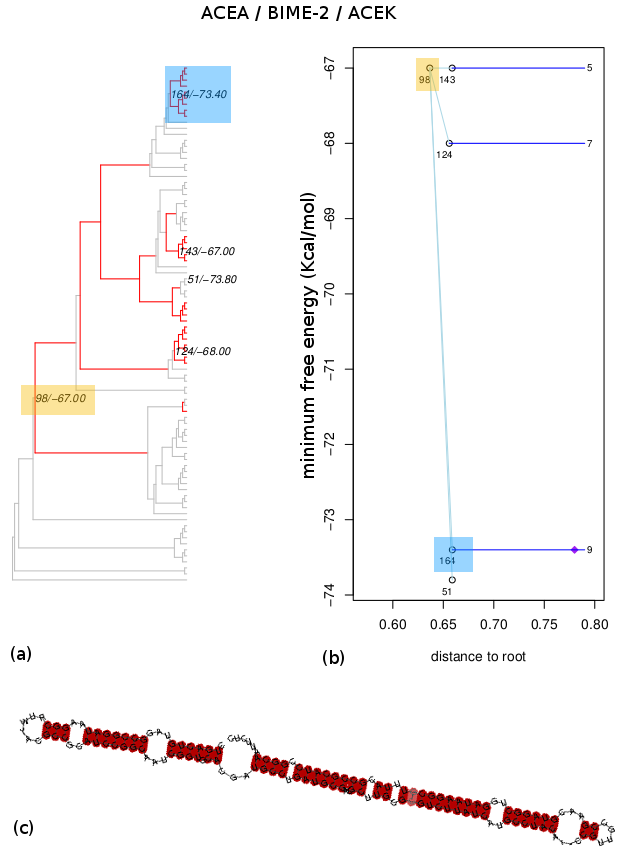
\includegraphics[scale=0.65]{figures/ancetre_ACEA_ACEK.png}
\caption{\textbf{Reconstruction des états ancêtres et calcul de l'énergie des structures secondaires pour la BIME flanquée des gènes aceA et aceK (opéron aceBAK). (a)} L'arbre phylogénique est une représentation de la reconstruction des séquences ancêtres, les longueurs des branches ne sont pas celles de l'arbre réel, elles ont été raccourcies par souci de représentation. Les branches rouges indiquent une conservation de la séquence, celles en gris indiquent des modifications telles que la perte d'une REP, une duplication de REP... L'identification des nœuds se fait par un numéro suivi par la valeur d'énergie minimale de la structure secondaire. \textbf{(b)} L'axe des abscisses représente la distance des nœuds à la racine, les ordonnées sont les valeurs d'énergie minimale des structures secondaires. Les numéros des nœuds correspondent à ceux de l'arbre phylogénique, les chiffres au bout des traits bleus foncés indiquent le nombre de souches dans le cluster et le losange violet marque la présence d'\textit{E. coli K12 MG1655} dans le cluster. Le nœud marqué en orange sur les 2 représentations est la séquence ancêtre la plus éloignée ayant conservée la séquence de la REP, celui marqué en bleu est celui du cluster contenant \textit{E. coli K12 MG1655}. \textbf{(c)} Représentation de la structure secondaire de la séquence consensus résultant des alignements de la BIME, en rouge sont annotées les zones conservées de l'alignement. Cette BIME fait partie de la famille des BIME-2 et est composée des REP : recY+ recZ2- recY+.}
\label{fig:ancetre} }
\end{SCfigure}

Nous nous donc sommes intéressés aux 11 résultats produits par GSE61327\_ALE que nous avons traités par la méthode de reconstruction des séquences ancêtres. Cette méthode produit un arbre phylogénique contenant les séquences ancêtres reconstruites à partir d'un arbre guide ainsi qu'une représentation de l'évolution de l'énergie minimale de la structure secondaire de l'ARN (\autoref{fig:ancetre}). Les résultats de l'analyse sont présentés en Annexe \ref{annexeAncetre}. Seul 10 résultats sont produits car le 11\up{ème} provient d'une BoxC+ unique annotée dans la base de données des REP de l'équipe. Les BoxC ne sont pas des REP et appartiennent à une autre famille d’éléments répétés, mais elles se trouvent souvent associées aux REP. Nous avons jugé préférable de l'exclure. \textcolor{red}{Sur les 10 résultats présentés, celui du couple hydN/hypF n'est pas utilisé pour la suite de l'analyse, car dans ce cas le second gène hypF est plus fortement exprimé sans la présence de promoteur.} L'énergie minimale de la structure secondaire est dépendante de la taille de la séquence de l'alignement (Données non montrées), cependant nous n'observons pas de tendance générale se dégageant sur la variation de cette valeur par rapport à l'énergie minimale de l'état ancêtre le plus éloigné. Nous observons à la fois des cas de stabilisation de la structure secondaire avec une diminution ou une conservation de l'énergie minimale dans 5 BIME sur 10 et des cas de déstabilisation semblant moins prononcés avec une augmentation de l'énergie minimale. Quand aux familles de BIME impliquées, il est intéressant de noter que les BIME-2 sont surreprésentées avec 60\% de présence (30\% sur l'ensemble du génome d'\textit{E. coli K12 MG1655}) au détriment des BIME solitaires et BIME-1.

\begin{SCfigure}[][h!]
\fbox{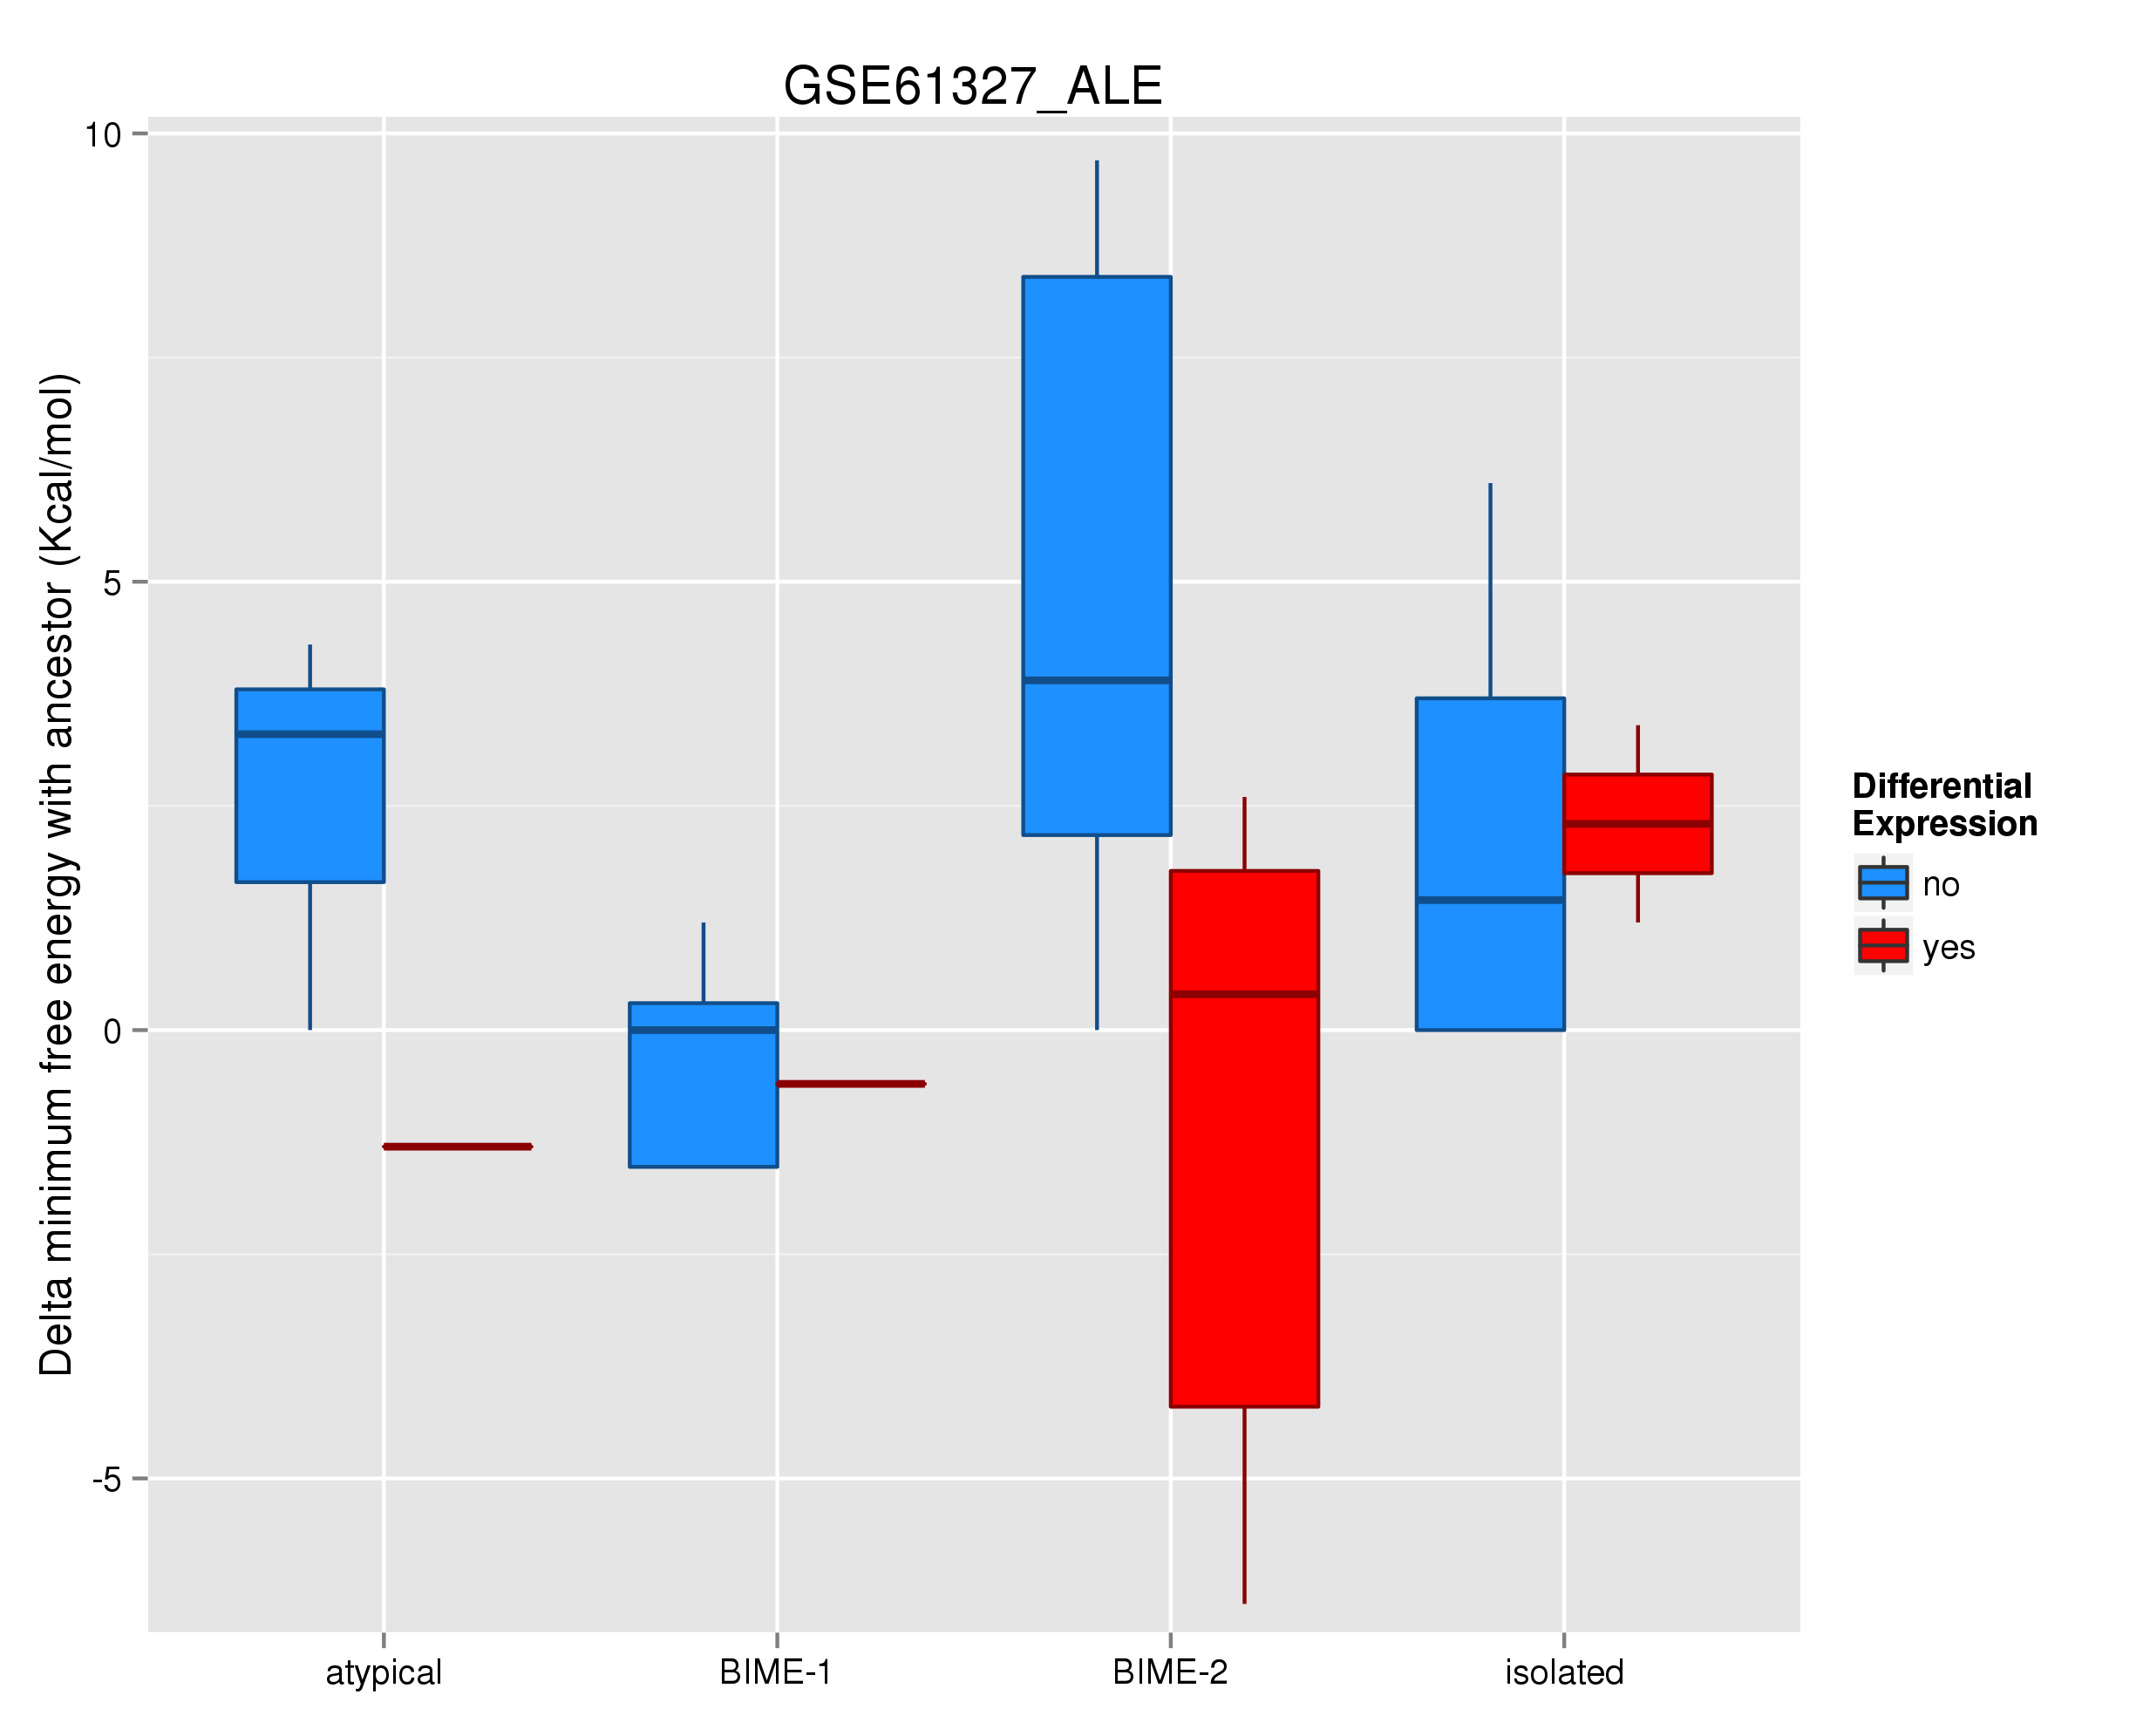
\includegraphics[scale=0.5]{figures/boxplot_ancestor_GSE61327_ALE.png}
\caption{\textbf{Distribution de l'évolution de l'énergie minimale de la structure secondaire des BIME par rapport à l'état ancêtre.} Le jeux de données est celui de l'expérience GSE61327\_ALE. L'axe des abscisses représente les différentes familles de BIME, l'axe des ordonnées représente la différence d'énergie minimale de la structure secondaire des BIME par rapport à l'état ancêtre le plus éloigné. Les données en rouge sont celles des BIME dont les 2 gènes flanquants sont DE, celles en bleu représentent les données des BIME dont les gènes flanquant ne sont pas DE.}
\label{fig:ancetreBoxplot} }
\end{SCfigure}

Nous avons ensuite appliqué le même traitement sur les 17 cas où dans un opéron en présence de BIME dans la RIG, nous n'observions pas de DE, ils sont présentés en Annexe \ref{annexeAncetre}. Sur ces 17 couples de gènes, un seul présente une BIME dont la structure secondaire s'est stabilisée, pour 6 cas nous n'avons pas de modification de l'énergie minimale de la structure secondaire et pour les 10 derniers cas nous observons une déstabilisation de la structure secondaire. Les proportions observées de chaque famille de BIME sont comparables aux proportions de chaque familles de BIME du génome d'\textit{E. coli K12} (Données non montrées).

La comparaison des distributions des différences d'énergie minimale avec la séquence ancêtre en fonction des familles de BIME et une DE des gènes flanquant la BIME (\autoref{fig:ancetreBoxplot}) nous permet d'observer la tendance pour toutes les familles de BIME vers une déstabilisation des structures secondaires dans le cas où il n'y a pas de DE. Cet effet apparaît nettement lorsque l'on s'intéresse aux BIME-2 avec un écart important entre les distributions avec et sans DE. Le cas des BIME atypiques semble similaire, mais est soumis à caution du fait du faible effectif dans le contexte d'une DE. Les BIME-1 sont soumises au même problème mais sans différence de distribution notable. La déstabilisation des BIME solitaires semble plus importante dans les cas de DE.
Un test de Chi2 d'indépendance sur les effectifs des différentes familles de BIME et en cas de DE ou non a conclu sur une indépendance des distributions (p-valeur : 0.7504).

La synthèse des résultats de notre étude est présentée sur la \autoref{fig:bilan}.

\begin{sidewaysfigure}
\centerline{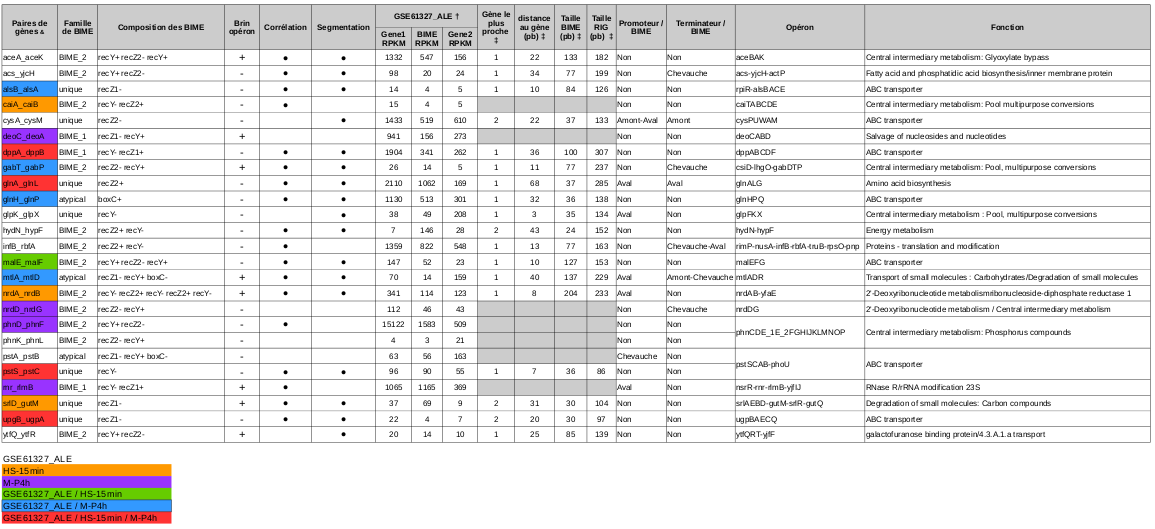
\includegraphics[scale=0.85]{figures/supData/synthese_french.png}}
\caption{\textbf{Tableau récapitulatif des résultats sur les trois jeux de données.} \& : Paires de gènes de l'opéron flanquant la BIME dont la différence d'expression est validée par un test statistique (p-valeur < 0.01). \dag~: Les données d'expression présentées sont uniquement celles de l'expérience GSE61327\_ALE par souci de clarté du tableau. \ddag~: Les données manquantes sont dues au fait que la méthode de calcul de proximité des gènes à la BIME, de la taille de la BIME, et de la taille de la région inter-génique n'ont été implémentés que dans la méthode de segmentation, ces informations sont donc liées à un résultat positif de cette méthode.}
\label{fig:bilan}
\end{sidewaysfigure}

\chapter*{Discussion}

\section*{Biais de séquençage des REP}
La première question que nous nous sommes posés est de savoir si nous pouvions nous fier aux données d'expression des REP, les résultats de la \autoref{fig:same_expression_operon_point} nous ont permis de constater un déficit du niveau d'expression des REP par rapport à ceux des gènes les flanquant alors que dans le cas des opérons que nous avons étudié nous nous attendions à ce que leur niveau d'expression soit au moins similaire à l'un des deux gènes. Les résultats des méthodes de localisation des points de cassures ont montré un déficit du taux d'expression des BIME du même ordre de grandeur. Plusieurs hypothèses peuvent expliquer ce biais, la première étant liée aux REP en elles-mêmes qui forment des structures secondaires pouvant avoir un effet sur la production de reads lors du séquençage. La seconde concerne la technique de préparation de la bibliothèque dans le contexte dans le contexte d'une expression des BIME en unités transcriptionnelles, puisque que dans le cas des études de DE en RNA-Seq, l'une des étapes consiste à faire une sélection du cDNA par la taille. Les REP solitaires et organisées en BIME-1 pouvant être plus fortement impactées que les BIME-2 ou BIME atypiques du fait de leurs tailles plus petites. La dernière hypothèse est liée au caractère répété des REP qui lors de l'alignement avec un logiciel tel que BWA peut produire des alignements à plusieurs endroits avec une valeur de qualité de mapping de zéro, comme nous avons décidé de les filtrer nous perdons certainement de l'information sur la couverture des BIME.

\section*{Expression des gènes dans les opérons et présence de BIME}
Grâce à l'indice $I_{expr}$, nous avons pu exploiter simplement les données d'expression de deux gènes consécutifs d'un opéron. En absence de BIME dans la RIG, les résultats sont conformes à ce que nous attendions, une distribution centrée sur zéro indiquant un niveau similaire d'expression des gènes et une distribution aplatie en présence des ET due à la contribution des promoteurs (gène 2 plus exprimé) et des terminateurs de transcription (gène 1 plus exprimé). La présence de BIME dans la RIG a pour effet notable d'augmenter le taux d'expression du gène 1 en présence ou non d'ET (\autoref{fig:expression_operon} (g-h-i)). La taille de la RIG ne semble pas être un facteur expliquant un niveau d'expression supérieur du premier gène, en revanche la localisation de la BIME à proximité du gène 1 paraît être un facteur important puisque dans 14 cas sur 18 observés de différence de niveau d'expression, la BIME se localise plus près du gène possédant le niveau d'expression le plus élevé.

L'étude de l'impact de la présence de promoteurs et de terminateurs dans la RIG sans BIME nous a démontré que dans tous les cas nous observions une différence avec l'$I_{expr}$ des gènes sans ET dans la RIG, alors qu'en présence de BIME, cette différence disparaît quasi complètement avec toujours un taux d'expression plus élevé du gène 1 (\autoref{table:p-val_reg}). La BIME joue donc un rôle dans le métabolisme de l'ARNm des opérons qui pourrait être celui d'atténuateur de transcription, notamment lorsque celle-ci chevauche un terminateur de transcription (14/39 BIME) ou un rôle de stabilisateur de la partie 5' du transcrit en le protégeant de l'action des exoribonucléases. Ces deux mécanismes mènent à la même constatation sur les données de RNA-Seq, un taux d'expression plus important du gène en amont de la BIME.






\chapter*{Conclusions et perspectives}

\end{onehalfspace}


% affichage du glossaire
\renewcommand{\thepage}{}
\printglossary[type=\acronymtype ,title=Glossaire]

%\bibliographystyle{unsrtnat}
\bibliography{biblio_rapport}

% annexes
\appendix

\chapter{}
\label{annexeCode}

Décompression du fichier au format \texttt{SRA} au format \texttt{fastq}, puis contrôle qualité des reads.
\lstset{language=sh, commentstyle=\color{ForestGreen}} 
\begin{lstlisting}[frame=single]
# Decompression
fastq-dump -Z file.sra > file.fastq
# Controle qualite
fastqc file.fastq
\end{lstlisting}

Alignement des reads des fichiers \texttt{fastq} sur le génome de référence, puis conversion du fichier \texttt{SAM} en fichier \texttt{BAM}. Tri du fichier \texttt{BAM} en fonction des positions génomiques. 
\lstset{language=sh, commentstyle=\color{ForestGreen}} 
\begin{lstlisting}[frame=single]
# Indexation du genome de reference
bwa index ref.fasta
# Alignement avec l'algorithme MEM de BWA
bwa mem ref.fasta file.fastq > aln.sam
# Conversion du SAM en BAM et application des filtres
# (-q 30: mapping minimal, -F 2048: pas de sequence chimeriques).
samtools view -Sbh -q 30 -F 2048 aln.sam > aln.bam
# Tri en fonction des positions genomiques
samtools sort aln.bam aln_sorted
\end{lstlisting}

Indexation du fichier \texttt{BAM} trié pour visualisation sur un Genome Browser. Fusion des différents fichiers \texttt{BAM} des réplicats en un seul fichier \texttt{BAM}.
\lstset{language=sh, commentstyle=\color{ForestGreen}} 
\begin{lstlisting}[frame=single]
# Indexation du fichier d'alignement
samtools index aln_sorted.bam
# Fusion des replicats.
samtools merge merged.bam aln_sorted_1.bam aln_sorted_2.bam \
aln_sorted_3.bam
\end{lstlisting}

Utilisation des BEDtools pour obtenir la couverture base par base sur une région d'intérêt.
\lstset{language=sh, commentstyle=\color{ForestGreen}}  
\begin{lstlisting}[frame=single]
# Couverture base par base.
bedtools coverage -abam merged.bam -b regionOfInterest.bed \
-d > unsorted_cov_perBase.bed
# Tri en fonction de la position genomique puis de la position 
# des bases dans chaque transcrit
sort -k2 -k7 -n unsorted_cov_perBase.bed | uniq > \
cov_perBase_strandToFix.bed
# Remplacement des '.' par des '*' dans la colonne des brins 
# pour l'utilisation sous R
awk 'BEGIN{OFS = "\t"} {gsub(/\./,"*",$6); print }' \
cov_perBase_strandToFix.bed > cov_perBase.bed
\end{lstlisting}

\chapter{}
\label{annexeOperon}
\begin{figure}[h!]
\centerline{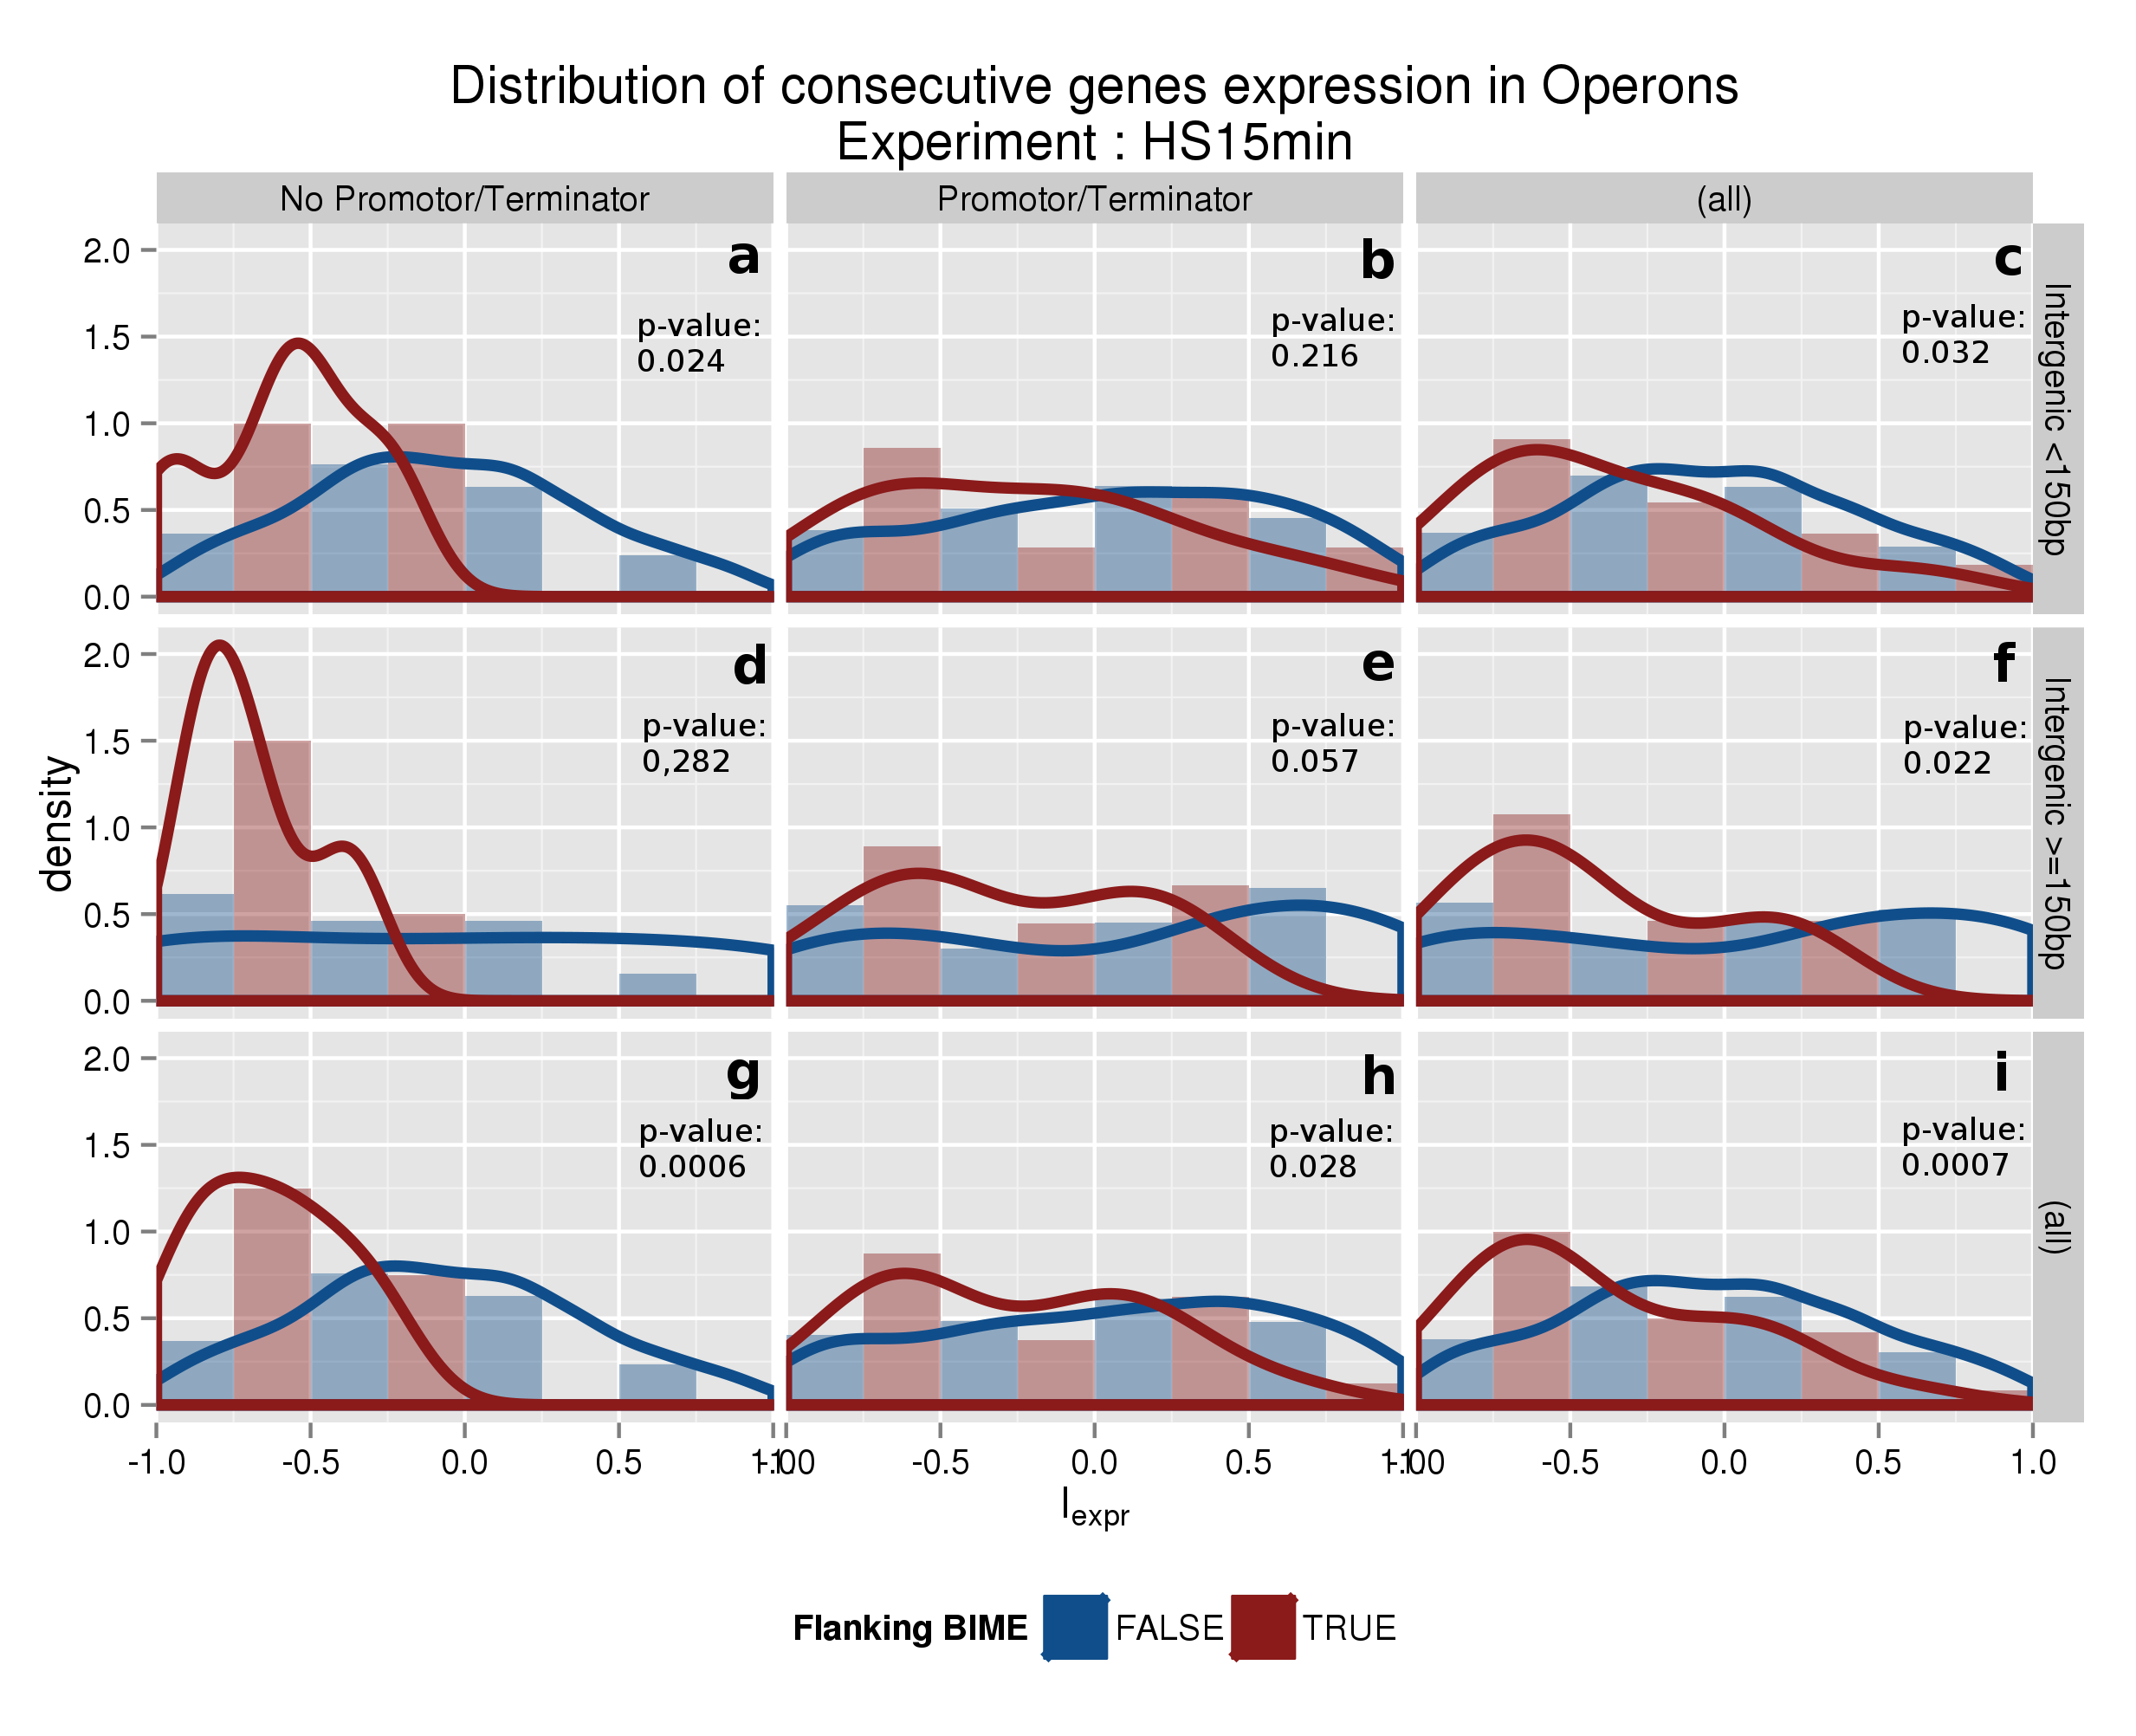
\includegraphics[scale=0.7]{figures/supData/genesOperon_histoDens_HS15.png}}
\caption{\textbf{Niveau d'expression des gènes consécutifs dans les opérons pour le jeux de données GSE61327\_ALE.}}
\end{figure}

\begin{figure}[!h]
\centerline{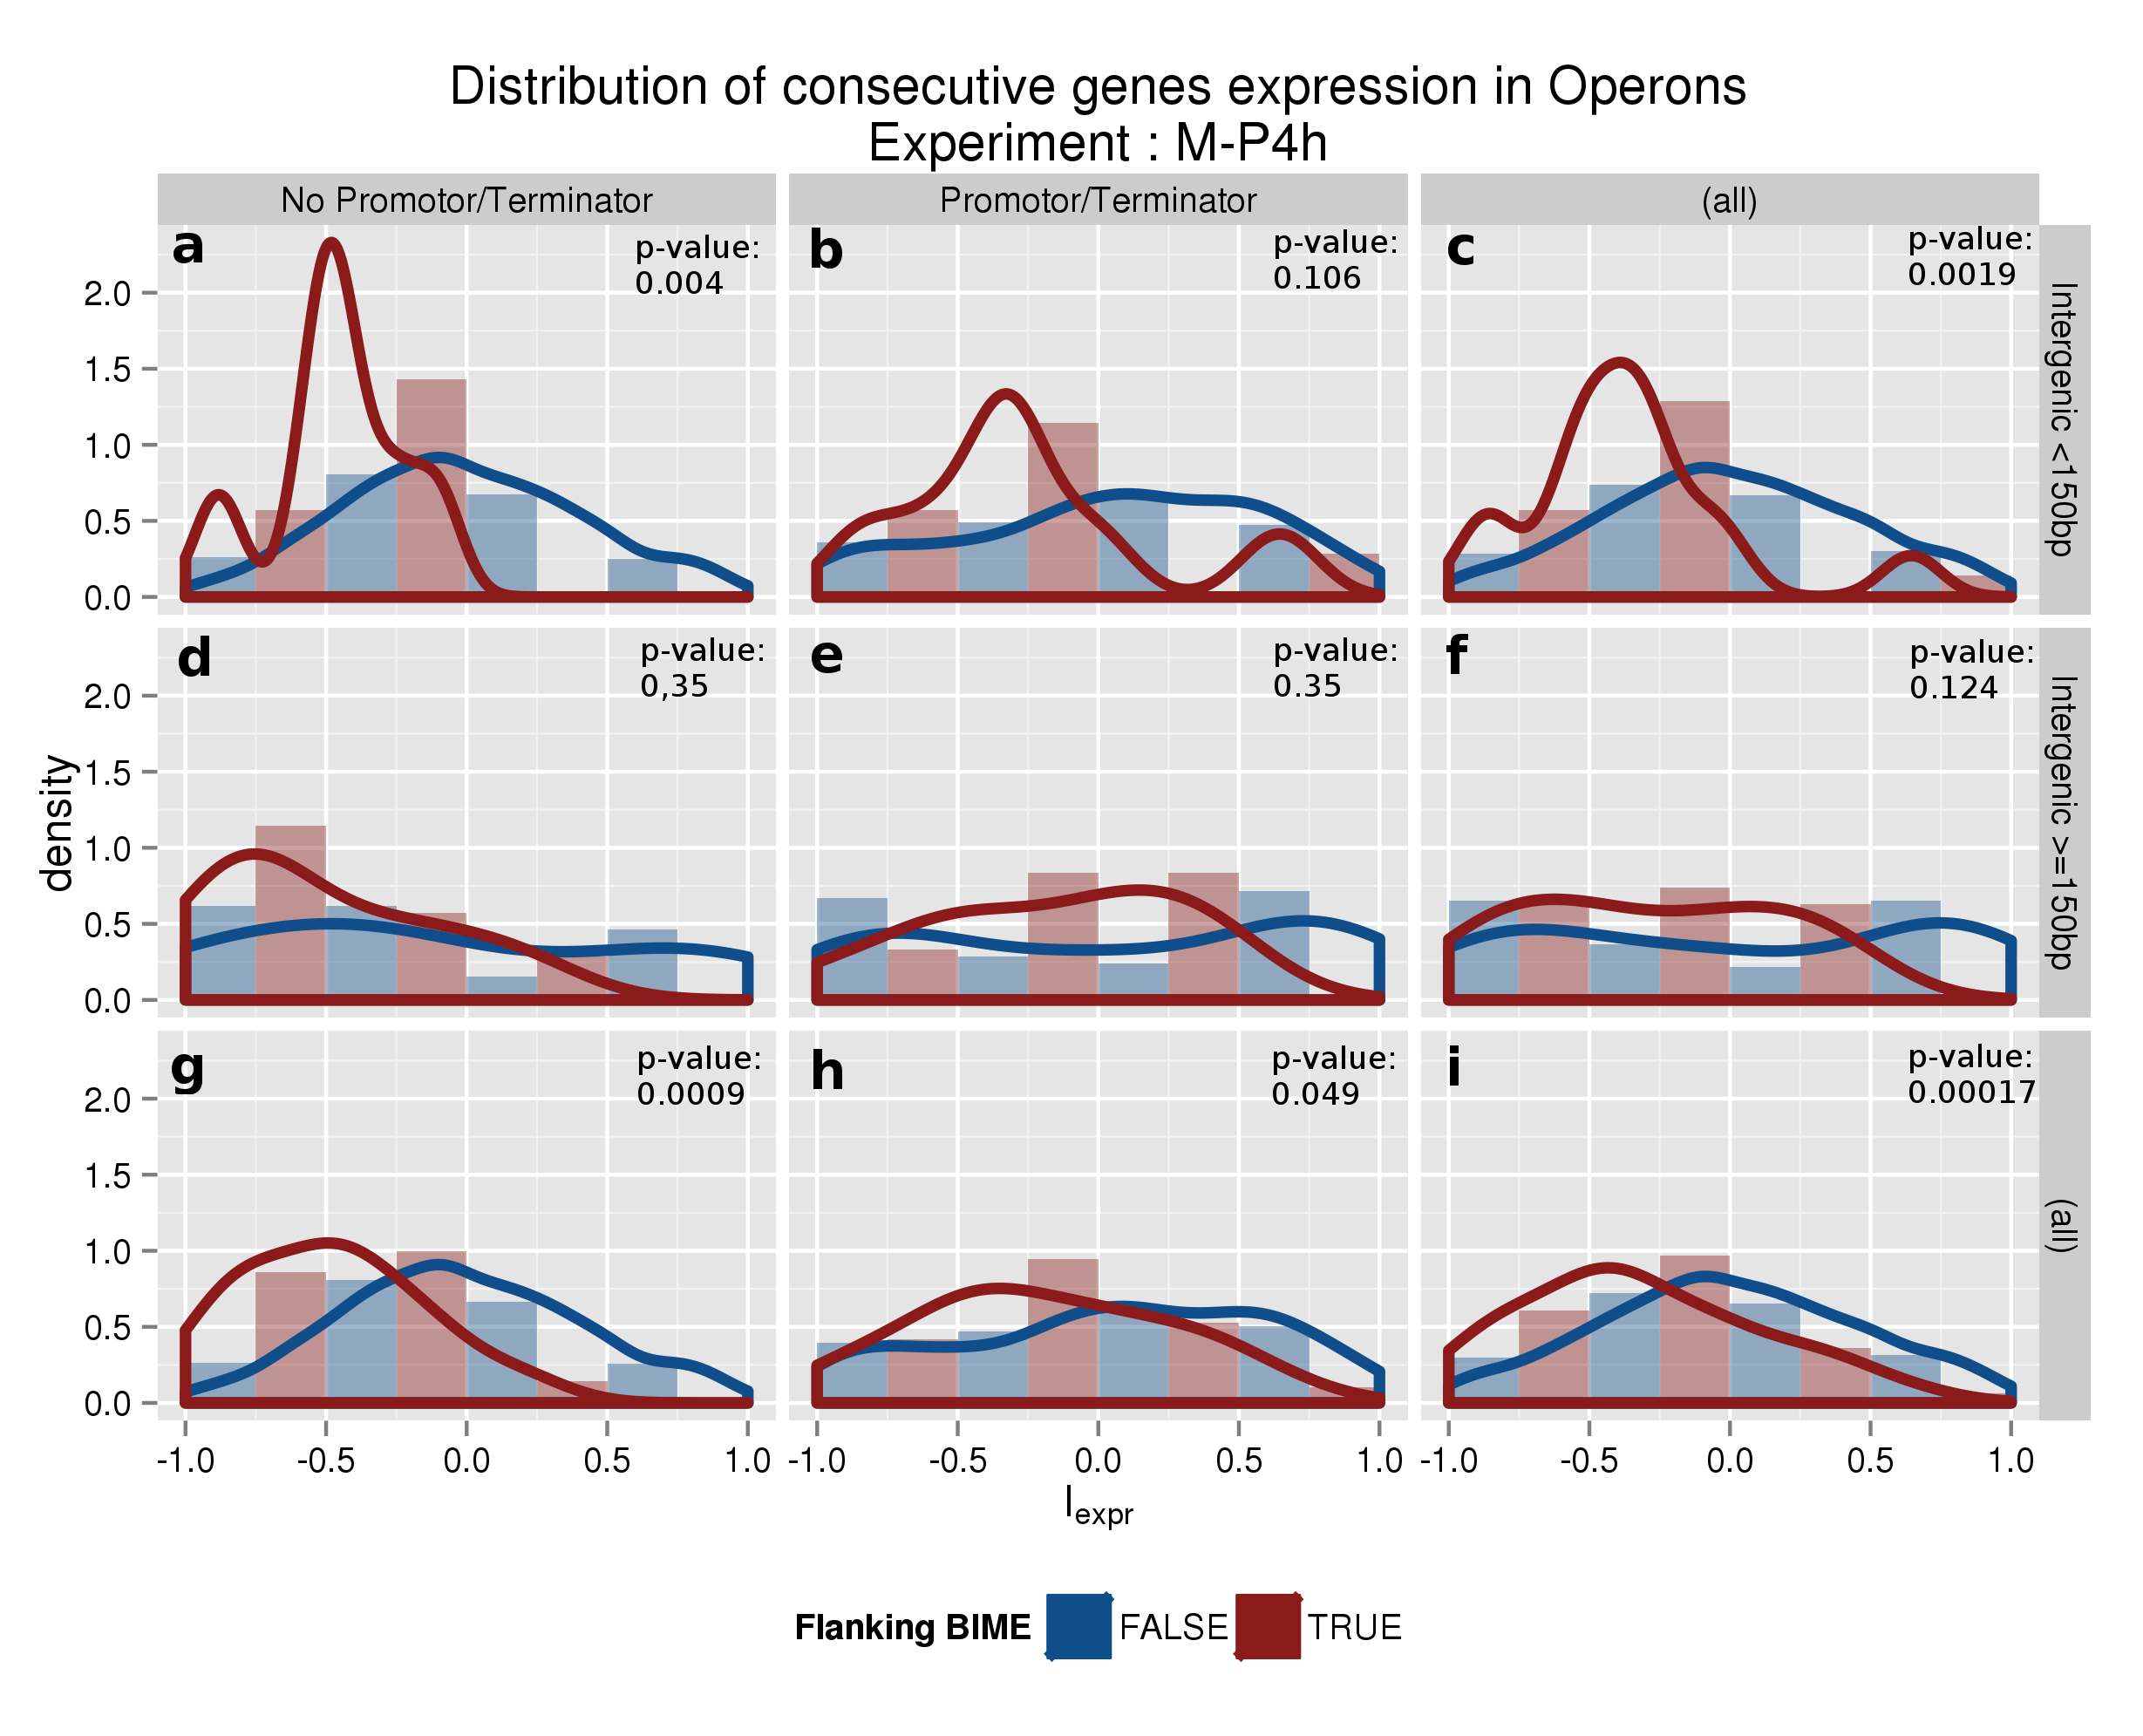
\includegraphics[scale=0.7]{figures/supData/genesOperon_histoDens_M-P4h.png}}
\caption{\textbf{Niveau d'expression des gènes consécutifs dans les opérons pour le jeux de données M-P4h.}}
\end{figure}

\chapter{}
\label{annexeVenn}
\begin{figure}[h!]
\centering
\subfigure[]{\label{fig:venn_GSE} 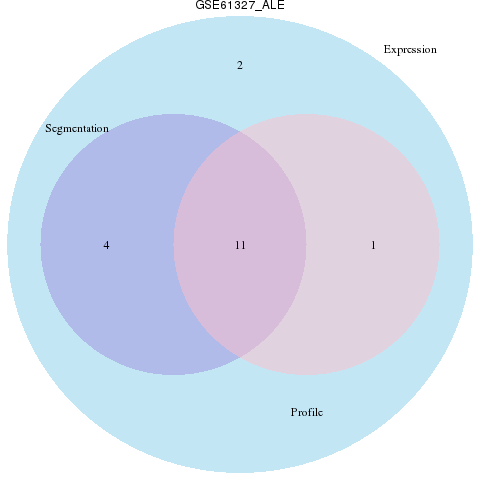
\includegraphics[scale=0.42]{figures/supData/venn_GSE61327_ALE.png}}
\subfigure[]{\label{fig:venn_HS} 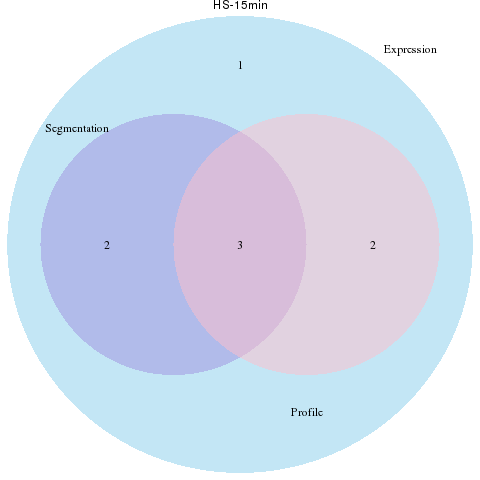
\includegraphics[scale=0.42]{figures/supData/venn_HS-15min.png}}
\subfigure[]{\label{fig:venn_MP} 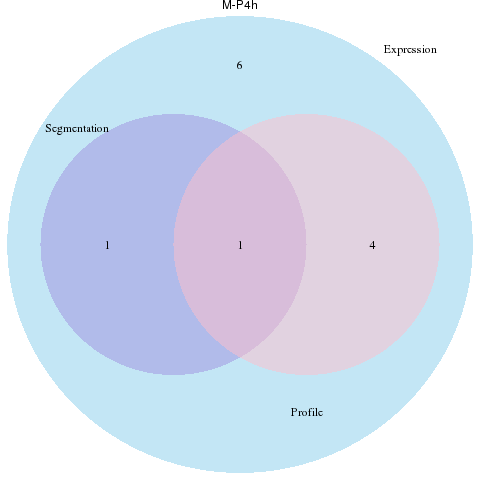
\includegraphics[scale=0.42]{figures/supData/venn_M-P4h.png}}
\caption{\textbf{Nombre de résultats trouvés pour chacune des 3 méthodes, Expression, corrélation de profils d'expression et segmentation. (a)} Données GSE61327\_ALE, 32 couples de gènes flanquant un BIME sont exprimés, pour 17 d'entre eux nous observons une DE et 11 sont retrouvés par les 3 méthodes. \textbf{(b)} Données HS-15min, 20 couples de gènes flanquant un BIME sont exprimés, pour 8 d'entre eux nous observons une DE et 3 sont retrouvés par les 3 méthodes. \textbf{(c)} Données M-P4h, 30 couples de gènes flanquant un BIME sont exprimés, pour 12 d'entre eux nous observons une DE et 1 seul est retrouvé par les 3 méthodes.} 
\end{figure}

\chapter{}
\label{annexeAncetre}
\begin{table}[h!]
\centerline{
\begin{tabular}{|l|c|c|c|c|c|c|c|}
  \hline
  \rowcolor{Gray}\begin{tabular}{c}Couples de gènes\\de l'opéron\end{tabular} & \begin{tabular}{c}Gène 1\\RPKM\end{tabular} & \begin{tabular}{c}Gène 2\\RPKM\end{tabular}  & \begin{tabular}{c}Nb. espèces\\dans le\\cluster \end{tabular} & \begin{tabular}{c}Énergie de\\la structure\\secondaire\end{tabular} & \begin{tabular}{c}$\Delta$ énergie\\sequence\\ancestrale\end{tabular} & \begin{tabular}{c}Famille\\de\\BIME\end{tabular}\\
  \hline
  mtlA\_mtlD & 70 & 159 & 35 & -62.8 & -1.3 & atypique\\
  \hline
  dppA\_dppB & 1904 & 262 & 19 & -39.1 & -0.6 & BIME-1\\
  \hline
  aceA\_aceK & 1332 & 156 & 9 & -73.4 & -6.4 & BIME-2\\
  \hline
  acs\_yjcH & 98 & 24 & 27 & -46.7 & +2.6 & BIME-2\\
  \hline
  gabT\_gabP & 26 & 5 & 25 & -44.8 & -5.6 & BIME-2\\  
  \hline
  hydN\_hypF & 7 & 28 & 45 & -47 & +2.1 & BIME-2\\
  \hline
  infB\_rbfA & 1359 & 548 & 32 & -40.1 & +0.8 & BIME-2\\
  \hline  
  malE\_malF & 147 & 23 & 20 & -70.1 & 0 & BIME-2\\
  \hline
  alsB\_alsA & 14 & 5 & 21 & -6.9 & +1.2 & solitaire\\
  \hline
  glnA\_glnL & 2110 & 169 & 21 & -20.7 & +3.4 & solitaire\\
  \hline  
\end{tabular}
}
\caption{\textbf{Résultats de la reconstruction des états ancêtres et de l'étude des structures secondaires pour les BIME des couples de gènes consécutifs avec différence d'expression dans les opérons.}}
\end{table}

\begin{table}[h!]
\centerline{
\begin{tabular}{|l|c|c|c|c|c|c|c|}
  \hline
  \rowcolor{Gray}\begin{tabular}{c}Couples de gènes\\de l'opéron\end{tabular} & \begin{tabular}{c}Gène 1\\RPKM\end{tabular} & \begin{tabular}{c}Gène 2\\RPKM\end{tabular}  & \begin{tabular}{c}Nb. espèces\\dans le\\cluster \end{tabular} & \begin{tabular}{c}Énergie de\\la structure\\secondaire\end{tabular} & \begin{tabular}{c}$\Delta$ énergie\\sequence\\ancestrale\end{tabular} & \begin{tabular}{c}Famille\\de\\BIME\end{tabular}\\
  \hline
  araA\_araD & 10 & 7 & 6 & -126.4 & +3.3 & atypique\\  
  \hline
  pstC\_pstA & 55 & 63 & 51 & -18.3 & +4.3 & atypique\\
  \hline
  sdhB\_sucA & 1606 & 984 & 30 & -63.7 & 0 & atypique\\
  \hline
  deoC\_deoA & 148 & 82 & 49 & -50.5 & 0 & BIME-1\\
  \hline
  fepA\_entD & 75 & 13 & 45 & -45.3 & 0 & BIME-1\\
  \hline
  flgF\_flgG & 384 & 361 & 26 & -46.9 & +1.2 & BIME-1\\
  \hline
  rnr\_rlmB & 292 & 179 & 40 & -53.1 & -6.1 & BIME-1\\
  \hline  
  caiA\_caiB & 33 & 15 & 25 & -45.1 & +9.7 & BIME-2\\
  \hline
  lamB\_malM & 104 & 81 & 22 & 69.1 & +1.8 & BIME-2\\
  \hline
  lspA\_fkpB & 536 & 387 & 20 & -58.8 & 0 & BIME-2\\
  \hline
  nrdA\_nrdB & 412 & 491 & 21 & -113.2 & +4.5 & BIME-2\\
  \hline
  nrdD\_nrdG & 97 & 19 & 9 & -29.6 & +27.2 & BIME-2\\
  \hline  
  sucB\_sucC & 1676 & 1729 & 10 & -85.5 & +3.3 & BIME-2\\
  \hline
  cysI\_cysH & 2417 & 1655 & 51 & -17.6 & 0 & solitaire\\
  \hline  
  nuoL\_nuoM & 375 & 505 & 26 & -25 & +6.1 & solitaire\\
  \hline
  srlD\_gutM & 23 & 30 & 48 & -18.2 & +2.9 & solitaire\\
  \hline
  yccB\_appA & 22 & 18 & 42 & -23.7 & 0 & solitaire\\
  \hline
\end{tabular}
}
\caption{\textbf{Résultats de la reconstruction des états ancêtres et de l'étude des structures secondaires pour les BIME des couples de gènes consécutifs sans différence d'expression dans les opérons.} }
\end{table}




\end{document}